\documentclass[a4paper,12pt,oneside, bibliography=totoc]
{scrbook}
\usepackage[utf8]{inputenc}
\usepackage{pgf-umlcd}
% Schrift und -kodierung
\usepackage[T1]{fontenc}
\usepackage{lmodern}
\usepackage{tcolorbox}
% Sprache/Silbentrennung
\usepackage[english]{babel} %TODO change to german if desired
\usepackage{booktabs}
\usepackage{amsmath}
\usepackage{floatflt}
\usepackage{float} 
\usepackage{verbatim}
\usepackage{hyperref}
\usepackage{graphicx}
\usepackage{pbox}
\usepackage{algorithmic}
\usepackage{algorithm}
\usepackage{subcaption}
\usepackage{siunitx}
\usepackage[autostyle]{csquotes}
\usepackage{todonotes}
\usepackage{svg}
\usepackage[page, title, titletoc, header]{appendix} %prettier appendix

\svgpath{{../figures/}}

\usepackage[printonlyused]{acronym}
\usepackage{listings} 
%\usepackage{subfig}
\lstset{xleftmargin=2em} %Proper indention of listings

\widowpenalty10000
\clubpenalty10000
\usepackage{tabularx} %For tables
\usepackage{csquotes} %For Quotes





%Footnote Numbering not reset in new chapters
\usepackage{chngcntr}
\counterwithout{footnote}{chapter}


%Remove last point after section/subsections
\renewcommand{\autodot}{}

\usepackage[htt]{hyphenat} %damit texttt noch Linebreaks mit Silbentrennung erzeugt
\newcommand{\code}[1]{\texttt{#1}} %Programmcode im Textfluss in passendem Font ausgeben

%Literatur
%Ordering in references checken, vermutlich was mit style=numeric zu tun
\usepackage[
   backend=biber,
   sorting= none,
   giveninits=true,
   date=long,
   urldate=long,
   url=false
]{biblatex}
\addbibresource{database.bib}
%\addbibresource{literatur2.bib}


\usepackage[]{hyperref}

\begin{document}
\frontmatter %roman page numbers





	\titlehead{
	\begin{center}
	   \includegraphics[width=10cm]{figures/unilogo.pdf}\\
	   	Institute of Computer Science, Software Engineering Group
	\end{center}
	}
	\subject{Master Thesis: }
	\title{ Refactoring data clumps with the help of ChatGPT
 }
	\author{Timo Schoemaker\\ Immatriculation number: 978621} %engl. Matriculation Number

	\date{\today\\
	Advisor: Prof. Dr.-Ing. Elke Pulvermüller \\ %Deutsch: Erstebetreuer
	Co-Advisor: Nils Baumgartner, M. Sc.} %Deutsch: Zweitbetreuer
	
	\maketitle
	
	\clearpage
	
	\addchap*{Abstract}
\textbf{Deutsch}

Code-Smells (z.~dt. übelriechender Code ) gelten als zuverlässiges Anzeichen für Quellcode mit Qualitätsprobleme, was zu höheren Wartungskosten führt. Refaktorisierungen von Code-Smells können diese Probleme lösen, haben aber in der Praxis nur eine geringe Priorität. Eine Lösung können automatisierte Refaktorisierungen sein, die den Entwickler bei der Behebung unterstützen. Der Fokus dieser Masterarbeit wird auf das Code-Smell „data clump“ (z.~dt. Datenklumpen) liegen, bei dem Variablen im Quellcode dupliziert werden. Bislang gibt es noch keine automatisierten Werkzeuge zur Behebung dieses Code-Smells. Mithilfe von Sprachmodellen wie ChatGPT, die  seit einiger Zeit große Aufmerksamkeit erregt haben,  wird ein modulares Werkzeug entwickelt, das die Detektion und Behebung von Data-Clumps automatisch durchführen kann.  Die Eignung von ChatGPT für diese Aufgabe wird  anschließend mittels einer Umfrage auf GitHub und anderen Experimenten untersucht. 
%\linebreak
\bigskip

\noindent
%\bigskip
\textbf{English} 
The existence of code smells is a reliable indicator for code quality issues which often induces higher maintenance costs. Refactoring code smells is an effective way to improve the quality of the code, but is not the priority of many developers.  Therefore, automatic refactoring tools can help to support developers to fix code smells. This master thesis focuses on one particular code  smell named data clumps, which is the duplication of variables across the code. No automatic refactoring tool for this code smell exists. Employing the capabilities of large language models such as ChatGPT that  recently have gained widespread attention, a modular tool is developed  that automatically detects and fixes data clumps. The thesis evaluates whether ChatGPT is suitable for this task via a GitHub pull request survey and other experiments. 




	\clearpage
	
	\tableofcontents
	\clearpage

	




\lstdefinelanguage{YAML}{
  morekeywords=
  {
    name:,on:,jobs:,steps:,uses:,run:,echo,workflow_dispatch:,description:,inputs:,required:,default:,runs-on:,using:,main:,with:,author:, absolute_threshold:
  },
  keywordstyle=\color{black}\bfseries,
  ndkeywords={false,compf/JavaDocEvaluator@action},
  ndkeywordstyle=\color{black}\bfseries,
  identifierstyle=\color{black},
  sensitive=false,
  comment=[l]{//},
  morecomment=[s]{/*}{*/},
  commentstyle=\color{purple}\ttfamily,
  %stringstyle=\color{red}\ttfamily,
  morestring=[b]',
  morestring=[b]",
  alsodigit={:},
  alsoletter={/,@,-}
}




\lstdefinelanguage{ANTLR}{
  keywords=
  {
   formalParameter:,variableModifier:,typeType:,variableDeclaratorId:,JCOMMENT:
  },
  keywordstyle=\color{black}\itshape,
  identifierstyle=\color{black},
  sensitive=false,
  comment=[l]{//},
  morecomment=[s]{/*}{*/},
  commentstyle=\color{purple}\ttfamily,
  morestring=[b]',
  morestring=[b]",
  alsodigit={:},
}

\lstdefinelanguage{JSON}{
    tabsize             = 4,
    showstringspaces    = false,
    keywords            = {false,true,include,exclude,metrics,metric_name,weight,unique_name,params,absolute_threshold,builder,relative_threshold},
    alsoletter          = 0123456789.*,
    ndkeywordstyle         = \color{red},
  keywordstyle=\color{black}\bfseries,
}





\lstdefinelanguage{javascript}{
  keywords={typeof, new, true, false, catch, function, return, null, catch, switch, var, if, in, while, do, else, case, break,let,this,private},
  keywordstyle=\color{black}\bfseries,
  identifierstyle=\color{black},
  sensitive=true,
  comment=[l]{//},
  morecomment=[s]{/*}{*/},
  commentstyle=\color{purple}\ttfamily,
  stringstyle=\color{red}\ttfamily,
  morestring=[b]',
  morestring=[b]",
}
%\ac{Abk.}         % fügt die Abkürzung ein, außer beim ersten Aufruf, hier wird die Erklärung mit angefügt
%\acs{Abk.}        % fügt die Abkürzung ein
%\acf{Abk.}        % fügt die Abkürzung UND die Erklärung ein
%\acl{Abk.}        % fügt nur die Erklärung ein

%\chapter*{Acronyms}
\addchap{Abkürzungsverzeichnis}

%%%%%%%%%%%%%%%%%%%%%%%
\begin{acronym}[E/E/PE] %sorgt fuer proper indention
	\acro{API}{\emph{Application Programming Interface}}
	\acro{AST}{\emph{Abstract Syntax Tree}}
	\acro{ATL}{\emph{Atlas Transformation Language}}
	\acro{BMWi}{\emph{Bundesministerium für Wirtschaft und Energie}}
	\acro{CIM}{\emph{Computation-Independent Model}}
	\acro{CDC}{\emph{Code-level design choice}}
	\acro{CR}{\emph{Code-level requirement}}
	\acro{CI/CD}{\emph{Continuous Integration/Continuous Delivery}}
	\acro{CRC}{\emph{Cycling Redundancy Checks}}
	\acro{E/E/PE}{\emph{Electrical/Electronic/Programmable Electronic}}
	\acro{ECC}{\emph{Error Detecting and Correcting Codes}} 
	\acro{EMF}{\emph{Eclipse Modeling Framework}}
	\acro{EGL}{\emph{Epsilon Generation Language}}
	\acro{EOL}{\emph{Epsilon Object Language}}
		\acro{HTML}{\emph{Hyper Text Markup Language}}
	\acro{Epsilon}{\emph{Extensible Platform of Integrated Languages for mOdel maNagement}}
	\acro{FS}{\emph{Functional Safety}}
	\acro{HAL}{\emph{Hardware Abstraction Layer}}
	\acro{HolMES}{\emph{Holistische Modell-getriebene Entwicklung für Eingebettete Systeme unter Berücksichtigung unterschiedlicher Hardware-Architekturen}}
	\acro{IDE}{\emph{Integrated Development Environment}}
	\acro{JSON}{\emph{JavaScript Object Notation}}
	\acro{JDT}{\emph{Java Development Tools}}
	
	\acro{LOC}{\emph{Lines of Code}}
 	\acro{LM}{\emph{Language Model}}

	\acro{MISRA}{\emph{Motor Industry Software Reliability Association}}
	\acro{MBU}{\emph{Multi Bit Upset}}
	\acro{MDA}{\emph{Model Driven Architecture}}
	\acro{MDC}{\emph{Model-level design choice}}
	\acro{MDD}{\emph{Model Driven Development}}
	\acro{MDE}{\emph{Model Driven Engineering}}
	\acro{MOF}{\emph{Meta Object Facility}}
	\acro{MR}{\emph{Model-level requirement}}
	\acro{NLP}{\emph{Natural Language Processing}}
	\acro{OCL}{\emph{Object Constraint Language}}
	\acro{OMG}{\emph{Object Management Group}}
	\acro{PIM}{\emph{Platform-Independent Model}}
	\acro{PSM}{\emph{Platform-Specific Model}}
	\acro{SER}{\emph{Soft Error Rate}}
	\acro{SEU}{\emph{Single Event Upset}}
	\acro{TMR}{\emph{Triple Modular Redundancy}}
	\acro{UML}{\emph{Unified Modeling Language}}
	


%\acro{cMOF}{\emph{complete MOF}}
%\acro{eMOF}{\emph{essential MOF}}

%	\acro{ETL}{\emph{Epsilon Transformation Language}}
%	\acro{EWL}{\emph{Epsilon Wizard Language}}

	
\end{acronym} %See inside for usage of acronmys
\mainmatter %switch roman auf arabic page numbers



\chapter{Introduction}
\setcounter{page}{1} %Seitenzahlen hier mit 1 anfangen

	%Include text from other files into the document --> great for structuring
	\label{sec:introduction}

Ein wichtiger Bestandteil der Softwareentwicklung von heute ist die Softwaredokumentation. Dies liegt unter anderem daran, dass die Größe von Softwareprojekten steigt, sodass die Entwickler schnell den Überblick über das Projekt verlieren können und daher zusätzliche Informationen neben dem Code benötigen \cite[S.~1]{StaticAnalysis:AnIntroduction:TheFundamentalChallengeofSoftwareEngineeringisOneofComplexity.}. Nichtsdestotrotz wird die Softwaredokumentation von Entwicklern oft vernachlässigt \cite[S.~83]{Qualityanalysisofsourcecodecomments}.  Die Gründe für schlechte Dokumentation sind vielfältig. Das Schreiben der Dokumentation wird oft als mühevoll empfunden und erfordert Fähigkeiten, die ein Programmierer nicht zwangsläufig besitzt \cite[S.~70]{AutomaticQualityAssessmentofSourceCodeComments:TheJavadocMiner} \cite[S.~593]{Softwareengineeringandsoftwaredocumentation:aunifiedlongcourse}.  

Weitere Studien verdeutlichen die Problematik der mangelhaften Softwaredokumentation. So belegt eine Umfrage aus dem Jahr 2002 mit 48 Teilnehmern  beispielsweise, dass die Dokumentation  bei Änderungen am System  nur mit Verzögerung angepasst wird. Knapp 70~\% der Teilnehmer stimmen der Aussage zu, dass die Dokumentation immer veraltet ist.   \cite[S.~28--29]{TheRelevanceofSoftwareDocumentationToolsandTechnologies:ASurvey}

Eine weitere Studie  \cite[S.~1199--1208]{SoftwareDocumentationIssuesUnveiled} aus dem Jahr 2019 verdeutlicht viele Aspekte aus der vorgenannten Umfrage. Es wurden dabei Daten aus Stack Overflow, GitHub-Issues, Pull-Requests und Mailing-Listen automatisiert heruntergeladen und dann von den Autoren analysiert, ob und inwieweit diese durch mangelhafte Softwaredokumentation verursacht wurden.  Die Studie belegt, dass von 824 Problemen, die etwas mit dem Thema \enquote{Softwaredokumentation} zu tun haben, 485 sich auf den Inhalt der Dokumentation beziehen (wie z.~B. unvollständige, veraltete oder sogar inkorrekte Dokumentation). Bei 255 Einträgen gab es Probleme mit der Struktur der Dokumentation, sodass beispielsweise Informationen schlecht auffindbar sind oder nicht gut verständlich sind.


Eine andere Umfrage aus dem Jahr 2014 mit 88 Teilnehmern zeigt, dass eine automatisierte Überprüfung der Dokumentationsqualität von knapp der Hälfte der befragten Entwickler gewünscht wird. Die Autoren der Studie sehen dies als Zeichen dafür, dass ein grundsätzliches Bedürfnis zur automatisierten Bewertung von Dokumentationen besteht und daher weitere Studien notwendig sind. \cite[S.~340]{TheValueofSoftwareDocumentationQuality}

Die mangelhafte Dokumentation führt dazu, dass nicht nur nachfolgende Entwickler Probleme mit dem Codeverständnis haben, sondern auch Entwickler eines Moduls nach einer längeren Pause Zeit aufbringen müssen, um den Code wieder zu verstehen \cite[S.~511]{vestdam}.  Auch für Kunden/Auftraggeber ist eine gute Dokumentation wichtig, da gut dokumentierte Software tendenziell besser wartbar ist und somit mehr Nutzen bringt \cite[S.~83]{Qualityanalysisofsourcecodecomments} \cite[S.~1]{SoftwareDocumentationManagementIssuesandPractices:ASurvey}.



\section{Zielsetzung}
Aufgrund der Relevanz von gut dokumentierter Software ist eine regelmäßige Rückmeldung über die Dokumentation von hoher Bedeutung. Spezielle Metriken, die eine numerische Auskunft über die Qualität der Softwaredokumentation liefern, sind eine Möglichkeit, diese Rückmeldung zu geben. Diese Metriken verschaffen dem Programmierer eine Einschätzung darüber, ob die Softwaredokumentation ausreichend ist oder eine Verbesserung sinnvoll wäre. Die Qualität der Softwaredokumentation kann auf unterschiedliche Art und Weise bewertet werden. So kann beispielsweise die bloße Existenz einer Dokumentation geprüft werden oder aber auch die Verständlichkeit der Dokumentation bewertet werden, daher kann es sinnvoll sein, mehrere Metriken zu verwenden \cite[S.~29]{pfleeger1992using}. Damit ein Entwickler einen Gesamtüberblick über die Dokumentationsqualität erhält, können diese Metriken kombiniert werden, um eine einzelne numerische Bewertung der Qualität der Dokumentation zu erhalten. 
Dabei ist es auch ratsam, die Metriken zu gewichten oder eine andere Methode zur Kombination der Metrikergebnisse zu benutzen, weil nicht jede Metrik die gleiche Zuverlässigkeit und Relevanz besitzt \cite[S.~1117ff.]{Softwarequalitymetricsaggregationinindustry}.

Damit das Feedback über die Softwaredokumentation auch wahrgenommen wird, sollte die Qualität regelmäßig  überprüft werden. Dies kann automatisiert im \ac{CI/CD}-Prozess erfolgen, bei dem Software kontinuierlich getestet und für den Release (z.~dt. Veröffentlichung) vorbereitet werden kann. Durch CI/CD können Unternehmen effizienter und besser Software entwickeln. So konnte das Unternehmen \textit{ING NL} die gelieferten Function-Points vervierfachen und die Kosten für einen Function-Point auf einen Drittel reduzieren \cite[S.~520]{Vassallo2016}.

\hfill

Basierend auf diesen Überlegungen soll ein Tool (z.~dt. Werkzeug) entwickelt werden. Dieses Tool (im Folgenden auch \textit{DocEvaluator} soll ein gegebenes Software-Projekt analysieren und eine numerische Bewertung abgeben, die eine heuristische Aussage über die Qualität der Softwaredokumentation trifft.  Dabei soll das Tool primär für Javadoc und Java bis Version 8 konzipiert werden, allerdings soll während der Entwicklung auch darauf geachtet werden, dass eine Portierung auf eine andere Programmiersprache ermöglicht wird und die Bewertung der Dokumentation unabhängig von der Programmiersprache funktioniert. Außerdem wird zur Vereinfachung nur englischsprachige Dokumentationen betrachtet. Komplexe \ac{NLP}-Metriken sollen dabei außer Acht gelassen werden. Auch Verfahren, die  den  Quellcode mit der Dokumentation vergleichen, wie z.~B. \textit{iComment} in \cite[S.~145ff.]{icomment}, sollen unberücksichtigt bleiben, da sie im Rahmen dieser Bachelorarbeit zu komplex sind. 

Dabei sollte es nicht unbedingt das Ziel sein, dass jede Komponente dokumentiert ist, sondern dass die wichtigen Komponenten eine gute Dokumentationsqualität haben und somit die Wartung vereinfacht wird. Als Komponente im Sinne dieser Bachelorarbeit werden dabei Klassen, Schnittstellen, Methoden und Felder verstanden. 

Dieses Tool soll anschließend in den \ac{CI/CD}-Prozess eingebunden werden, sodass die Dokumentationsqualität kontinuierlich geprüft werden kann. Als \ac{CI/CD}-Plattform soll dabei \textit{GitHub Actions} \cite{GithubActions} verwendet werden, da GitHub von der Mehrzahl der Entwickler und großen Unternehmen verwendet wird \cite{github_popular}. Mittels GitHub Actions soll das Tool bei einer sehr schlechten Dokumentationsqualität den Entwickler auf diesen Umstand hinweisen, indem beispielsweise ein Merge (z.~dt. Verschmelzung) in GitHub verhindert wird. Auch bei einer deutlichen inkrementellen Verschlechterung der Qualität soll der Entwickler informiert werden, um so eine ausreichende Qualität der Dokumentation sicherzustellen. 

Ein Forschungsziel dieser Bachelorarbeit ist es zu prüfen, wie das Programm konzipiert werden muss, um mehrere Programmiersprachen zu unterstützen. Ein weiteres Ziel der Arbeit beschäftigt sich mit der Frage, wie die Ergebnisse der Metriken kombiniert werden können, um eine präzise Aussage über die Gesamtqualität der Dokumentation eines Softwareprojektes zu erhalten. Die Konzeption einer Architektur, mit der weitere Metriken hinzugefügt werden können und der Nutzer des Tools auswählen kann, welche Metriken bei der Bewertung der Dokumentationsqualität berücksichtigt werden sollen, soll ebenfalls als Forschungsziel untersucht werden. Zuletzt soll als Forschungsfrage diskutiert werden, welche Metriken eine heuristische Aussage über die Qualität der Dokumentation treffen können. 


\section{Gliederung}
In Kapitel \ref{sec:background} werden die wichtigen Grundlagen über die Themen dieser Bachelorarbeit erläutert. Dazu  wird zunächst der Begriff Softwaredokumentation definiert und ein Bezug zu Code-Smells hergestellt. Mittels Javadoc wird dann erläutert, wie Software dokumentiert werden kann. Anschließend wird eine Einführung in GitHub Actions gegeben.  Zudem wird eine Einführung in ANTLR4 gegeben, das für das Parsing der Quellcodedateien in Java verwendet wird. Zuletzt werden einige wissenschaftliche Arbeiten mit vergleichbaren Zielsetzungen präsentiert und Tools vorgestellt, die ebenfalls die Qualität der Softwaredokumentation bewerten können.

In Kapitel \ref{chapter_conception} werden die Fragestellungen besprochen, die sich beim Design des Tools ergeben haben. Dazu gehören die notwendigen Objekte und ihre Interaktion untereinander und wie von einer losen Ansammlung von Dateien zu einer Bewertung der Softwaredokumentation gelangt werden kann.

In Kapitel \ref{chapter:program} wird anschließend erläutert, wie aus dieser Konzeption ein vollständiges Programm entwickelt wird. Dazu wird erläutert, wie das Programm in GitHub Action eingebunden werden kann. Im Anschluss daran wird ein Überblick über die implementierten Metriken mit ihren Vor- und Nachteilen gegeben. Außerdem werden die Algorithmen bzw. Verfahren erläutert, um die Ergebnisse der einzelnen Metriken zu einem Gesamtergebnis zu aggregieren. 

In Kapitel \ref{sec:evaluation} wird das Programm dann mit ähnlichen Tools verglichen, indem beispielhafte Java-Projekte aus GitHub mit allen Programmen analysiert werden und die Geschwindigkeit und die Qualität jedes Programmes ermittelt wird. 

Im abschließenden Kapitel wird der Inhalt der Arbeit zusammengefasst und ein Fazit gezogen. Es werden offengebliebene Fragen beleuchtet und ein Ausblick gegeben, welche Möglichkeiten zur Verbesserung des Tools sinnvoll wären. 

\begingroup
\renewcommand{\cleardoublepage}{} % TODO maybe removing this and next
\renewcommand{\clearpage}{}
\chapter{Background}\label{chapter:background}
\endgroup

	%Multiple input files for larger chapters are also possible
In this chapter, the background of data clumps will be discussed. A formal definition of data clumps will be presented (\ref{sec:data_clumps}. ChatGPT will be discussed in section \ref{sec:chatgpt}. Also, there will be a discussion of the data clump type context format. 

\section{Data clumps}\label{sec:data_clumps}

A more precise and algorithmic  definition of \enquote{data clumps} is provided by \cite{zhangImprovingPrecisionFowler2008}. According to them, a data clump  can be defined on the field or method-parameter levels. 
To be a method parameter data clump, a group of at least three variables must appear in multiple methods. Those variables must be duplicated, meaning they share the same name and data type. However, the inner order of the group does not need to be the same. 

These conditions often need to be more relaxed. For instance, methods can be inherited and overridden so that a group of parameters may appear in each derived class thereby fulfilling the definition of a method parameter data clump. Since (except for the identifiers of the parameters) an overriding method must be the same as the overridden method, they are not considered data clumps. \cite{zhangImprovingPrecisionFowler2008}

To be a field data clump, similar conditions apply. There must be at least three fields that appear in more than one class and the names and data types of the variables must the same while the inner order may be different. Since in most programming language, a field can have an additional access modifier (e.g. \textit{private}, \textit{static} etc. ), the access modifier should also be included to determine whether two groups of variables are identical and hence a data clump.  \cite{zhangImprovingPrecisionFowler2008}

The definition might also need to be more relaxed for both method and field data clumps. Two variables, that have the same name but a compatible type in at least one direction  (e.g. \textit{int} and  \textit{double}), would be disregarded as a data clump according to the formalized definition, although some would regard them a data clump.

Also, modification of a variable's identifier might not change its meaning. For instance, typos can happen, or synonyms can be used so that an automatic algorithm might not discover the connection of two variables but requires  knowledge of the semantics of the source code. \cite{zhangImprovingPrecisionFowler2008}


To conclude, the core definition of a data clump is clear. However, this definition still leaves out some edge cases that require a semantic understanding of the source code.  




\begingroup
\renewcommand{\cleardoublepage}{} % TODO maybe removing this and next
\renewcommand{\clearpage}{}
\chapter{Konzeption}\label{chapter_conception}
\endgroup
Im Folgenden wird ein Konzept für die Implementierung des Tools vorgestellt, das die Ziele der Bachelorarbeit erfüllen soll. Um diese Ziele zu erreichen, müssen zuerst die Dateien geparst werden, was in Kapitel \ref{chapter:parsing} besprochen wird. Im darauffolgenden Kapitel \ref{chapter:metric_conception} wird erläutert, wie die extrahierten Informationen von den Metriken verarbeitet werden. 


\hfill
\section{Parsing von Dateien}\label{chapter:parsing}
Eine Quellcodedatei besteht zunächst aus reinem Text und bietet daher nur indirekt Einblick in die innere Struktur. Damit eine Bewertung der Dokumentationsqualität möglich ist, müssen bestimmte Strukturen aus einer Datei gelesen werden, die für die Dokumentation wichtig sind. Andere Strukturen können dabei ignoriert werden. Für die Bewertung der Dokumentation sind nur wenige Bestandteile relevant. Beispielsweise sind alle Conditional-Branches (wie z.~B.  For-Schleifen und If-Verzweigungen) und viele andere Komponenten in Methodenrümpfen nicht relevant, da diese nur mit normalen Kommentaren und nicht mit Javadoc kommentiert werden (sie werden dennoch unstrukturiert als Zeichenkette gespeichert, damit Metriken diese Information eventuell nutzen können). Aus diesem Grund müssen die notwendigen Informationen extrahiert werden. Zudem ist es ein Ziel der Arbeit, eine Erweiterbarkeit auf andere objektorientierte Programmiersprachen zu ermöglichen. Daher müssen die Informationen in ein abstraktes Format gebracht werden, welches eine gute Annäherung für die meisten objektorientierten Programmiersprachen ist. Beispielsweise unterscheiden sich die Zugriffsmodifizierer vieler Programmiersprachen, sodass eine einheitliche Schnittstelle schwer umsetzbar ist. Daher enthält die abstrakte Repräsentation nur Informationen darüber, ob eine Komponente als öffentlich markiert ist. Dies ist sinnvoll, da öffentliche Komponenten als Teil der öffentlichen Schnittstelle eher dokumentiert werden sollten als nicht öffentliche und eine weiter gehende Differenzierung kaum Vorteile bietet. In einigen Programmiersprachen wie z. B. Python gibt es keine expliziten öffentlichen Komponenten, jedoch existieren de facto Standards für Bezeichner, sodass beispielsweise private Komponenten zwei Unterstriche als Präfix haben.

Außerdem werden in der abstrakten Repräsentation die Vererbung etwas vereinfacht dargestellt, indem nicht zwischen Basisklassen und Schnittstellen unterschieden wird, da es auch hier Unterschiede zwischen Programmiersprachen gibt. Zudem werden Konstruktoren als Methoden mit den Namen \enquote{constructor} und Schnittstellen als Klassen repräsentiert, da auch hier eine zu feine Spezifikation nicht notwendig sein wird.  

  

In anderen Fällen gibt es jedoch viele Gemeinsamkeiten zwischen objektorientierten Programmiersprachen. So gibt es in  allen relevanten Sprachen Klassen, Methoden und Felder, die alle einen Namen haben. Des Weiteren haben Methoden und Felder einen (Rückgabe-)Typen und Methoden besitzen Parameter, die ihrerseits durch einen Namen und einen Typen definiert sind. Einige Sprachen sind zwar nicht stark typisiert, jedoch kann für nicht bekannte Datentypen ein Alias wie \enquote{Any} oder  \enquote{Object} verwendet werden.  Zudem sind viele Komponenten hierarchisch. In den meisten Sprachen können beispielsweise Klassen andere Klassen enthalten, sodass diese abstrakte Struktur diese Tatsache berücksichtigen müsste. 

Um dennoch sprachspezifische Funktionen anbieten zu können, besitzt jede Komponente ein Feld mit dem Typen \textit{ComponentMetaInformation}, das wie oben erwähnt die Information enthält, ob eine Komponente als öffentlich angesehen werden soll. Dieser Typ, welches eine Schnittstelle ist, kann von einer Klasse implementiert werden, um Parser für andere Programmiersprachen die Möglichkeit zu geben, zusätzliche sprachspezifische Informationen zu speichern. Beim Java-Parser wird diese Funktion beispielsweise genutzt, um zu speichern, welche \enquote{checked} Ausnahmen eine Methode werfen kann, sodass später ein Vergleich mit dem Javadoc-Block möglich ist. Die Schnittstelle enthält nur die Anforderung, eine \textit{isPublic}-Methode anzubieten und kann daher für viele andere objektorientierte Programmiersprachen Informationen speichern, die für einige Metriken eventuell nützlich sind. 



 \begin{figure}[ht!]
 \centering
 \scalebox{0.8}{
 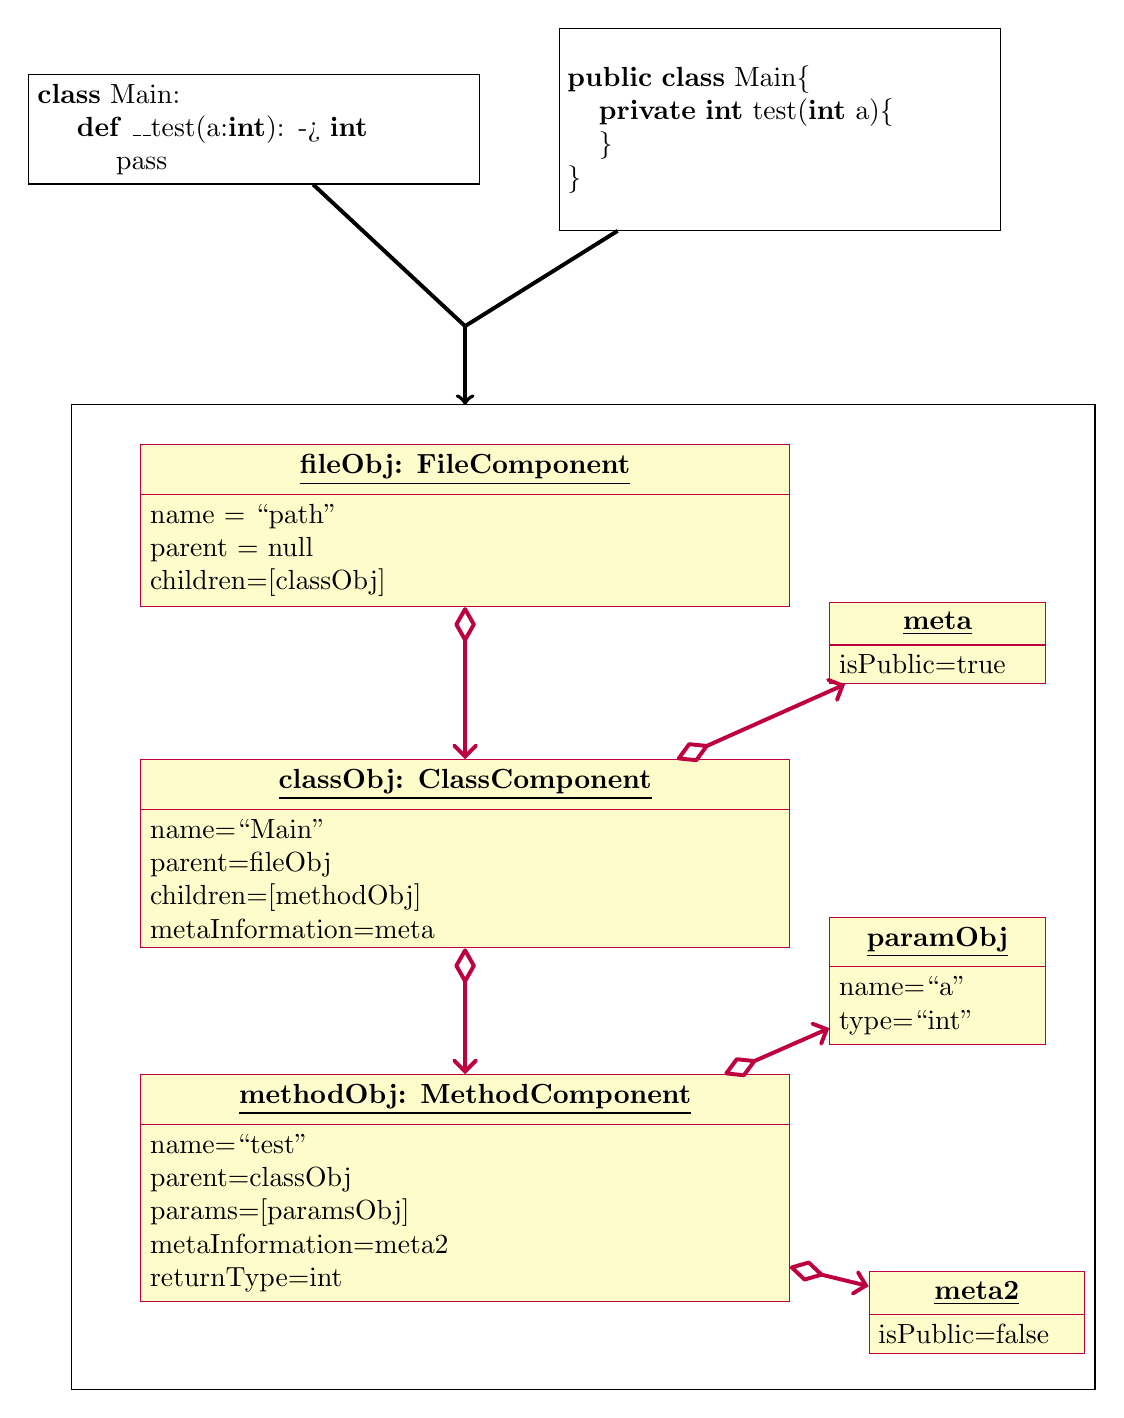
\begin{tikzpicture}
 \pgfmathsetlengthmacro\breite{6cm}
\pgfmathsetlengthmacro\hoehe{2.567cm}
\pgfmathsetlengthmacro\InnerSep{0.4cm}
\node[draw,
anchor=center, 
inner sep=0pt, 
minimum width=5cm, text width=6cm-\InnerSep,
align=justify,
minimum height=\hoehe
] (java) {
  \hspace*{0.1cm}\textbf{public} \textbf{class} Main\{\newline 
     \hspace*{0.5cm}\textbf{private} \textbf{int} test(\textbf{int} a)\{\newline
    \hspace*{0.5cm}\}\newline
\hspace*{0.1cm}\}

};
\node[draw,text width=5.5cm, left = of java](python){
\textbf{class} Main:\newline
     \hspace*{0.5cm}\textbf{def} \_\_test(a:\textbf{int}): -> \textbf{int}\newline
         \hspace*{1cm}pass

};
\draw[line width=0.05cm] (python) -- (-4,-2.5) ;
\draw [line width=0.05cm](java) -- (-4,-2.5);
\draw[->,thick,line width=0.05cm] (-4,-2.5) -- (-4,-3.5);
\draw [] (-9,-3.5) rectangle(4,-16);
\begin{scope} {0,-10}
       \begin{object}[text width=8cm]{fileObj}{-4,-4}
        \instanceOf{FileComponent}
        \attribute{name = \enquote{path}}
        \attribute{parent = null}
        \attribute{children={[}classObj{]}}
      \end{object}
      \begin{object}[text width=8cm]{classObj}{-4,-8 }
        \instanceOf{ClassComponent}
        \attribute{name=\enquote{Main}}
        \attribute{parent=fileObj}
        \attribute{children={[}methodObj{]}}
          \attribute{metaInformation=meta}
      \end{object}
    \begin{object}[text width=8cm]{methodObj}{-4,-12}
        \instanceOf{MethodComponent}
        \attribute{name=\enquote{test}}
        \attribute{parent=classObj}
        \attribute{params={[}paramsObj{]}}
        \attribute{metaInformation=meta2}
        \attribute{returnType=int}
      \end{object}
      \begin{object}[text width=2.5cm]{paramObj}{2,-10}
        \attribute{name=\enquote{a}}
        \attribute{type=\enquote{int}}
      \end{object}
    \begin{object}[text width=2.5cm]{meta}{2,-6}
        \attribute{isPublic=true}
      \end{object}
    \begin{object}[text width=2.5cm]{meta2}{2.5,-14.5}
        \attribute{isPublic=false}
      \end{object}
\end{scope}
\begin{scope}[line width=0.05cm]
    \aggregation{fileObj}{}{}{classObj}{}{}
     \aggregation {classObj}{}{}{methodObj}{}{}
      \aggregation {methodObj}{}{}{paramObj}{}{}
    \aggregation {classObj}{}{}{meta}{}{}
        \aggregation {methodObj}{}{}{meta2}{}{}
\end{scope}

    
\end{tikzpicture}
}
     
     \caption{Objektdiagramm aus Java- und Python-Code}
     \label{fig:python_java_comp}
 \end{figure}

Abbildung \ref{fig:python_java_comp} veranschaulicht, wie eine einfache Datei in die Objektstruktur umgewandelt werden kann. Dabei werden eine einfache Java-Datei und eine semantisch äquivalente Python-Datei als Beispiel verwendet, um zu zeigen, dass aus beiden Sprachen eine gleiche Objektstruktur erzeugt werden kann. Dabei wurden zur Übersichtlichkeit einige nicht relevanten Attribute entfernt.



Das Programm in beiden Sprachen besteht aus einer öffentlichen Klasse \textit{Main} und einer privaten Methode \textit{test}, die einen Parameter \textit{a} als Ganzzahl erhält und eine Ganzzahl zurückgibt. Die höchste Hierarchieebene ist immer ein \textit{FileComponent}. Diese Datei enthält hier genau ein Kind namens \textit{classObj}, könnte aber in anderen Fällen auch mehrere Kinder (wie z.~B. Klassen enthalten). Die Klasse besitzt zudem einen Verweis auf ihren Elternteil. Außerdem enthält das \textit{classObj} eine Referenz auf Metainformationen, die hier nur angeben, dass die Klasse öffentlich ist. In diesen Metainformationen könnten auch andere relativ sprachspezifische Informationen definiert werden, falls sie für Metriken relevant sein könnten. Die Klasse enthält wiederum genau die Methode als einziges Kind. Die Methode hat ebenfalls einen Verweis auf die Metainformationen, welche die Methode als privat markieren. Außerdem hat die Methode einen \textit{returnType} und einen Verweis auf die Liste der Parameter, die wiederum aus einem Namen und einem Datentyp bestehen. Das Feld \textit{comment}, welches einen Verweis auf den strukturierten Kommentar liefert, wird in dieser Abbildung nicht dargestellt, da es bei den Dateien keine Dokumentation gibt und es somit den Wert \textit{null} hat.

Die Beziehungen der Klassen, die für das Parsing zuständig sind, werden zusätzlich in Abbildung \ref{fig:uml_parsing} im Anhang \ref{appendix_parsing_uml}. als UML-Diagramm illustriert.

\subsubsection{Repräsentation der strukturierten Kommentare}\label{chapter:structured_comments}
Neben der hierarchischen Repräsentation der einzelnen Komponenten müssen auch die strukturierten Kommentare (wie z.~B. Javadoc) geeignet in eine Datenstruktur umgewandelt werden. Wie in Kapitel \ref{chapter:javadoc}
 erläutert, besteht ein strukturierter Kommentar in vielen Fällen aus zwei Teilen. Der erste Teil ist eine allgemeine Beschreibung der Komponente. Im zweiten Teil werden bestimmte Strukturen genauer erläutert. So können einzelne Parameter erklärt werden oder der Rückgabewert beschrieben werden. 
 Dieser Aufbau findet sich auch in \textit{Doxygen} \cite{doxygen} oder \textit{Docstring} \cite{docstring}, sodass diese Struktur als Grundlage genommen wird. 
 
 Ein strukturierter Kommentar besteht also aus einer generellen Beschreibung, die auch weggelassen werden kann. Anschließend folgen null bis beliebig viele Tags. Jeder Tag besteht aus einem Typ (z.~B. \enquote{@param}, \enquote{@return} oder \enquote{@throws}), einem optionalen Parameter, welcher von einigen Tags benötigt wird und der Beschreibung des Tags. Die Namen der Tags sind generalisiert, dies bedeutet, dass unabhängig von der Programmiersprache der Tag zur Beschreibung eines Parameters immer \enquote{@param} heißen muss. Dies muss bei der Entwicklung eines Parsers beachtet werden. 
 
 Ein strukturierter Kommentar kann ebenfalls spezielle Elemente (wie z.~B. \ac{HTML}-Elemente oder Inline-Tags) enthalten. Hier werden diese Elemente unverarbeitet gelassen, also unverändert mit dem Rest des Kommentars als Zeichenkette gespeichert. Metriken, die diese Informationen benötigen, müssen diese Elemente also selbstständig extrahieren. Andere Metriken (wie z.~B. die Metriken in Kapitel \ref{chapter:metrics_semantic}) benötigen diese speziellen Elemente nicht, sodass eine einheitliche Schnittstelle, die sowohl die natürliche Sprache als auch die speziellen Elemente berücksichtigt und  zudem relativ programmiersprachenunabhängig sein müsste, viele Herausforderungen mit sich bringt.   
 
 Wird kein strukturierter Kommentar angegeben, so liefert der entsprechende Getter \textit{getComment} den Wert \enquote{null} zurück. 
\section{Konzeption der Metriken}\label{chapter:metric_conception}
Nachdem eine Datei in ihre einzelnen Komponenten zerlegt wurde, kann die Qualität der Softwaredokumentation überprüft werden. Jede gefundene Komponente besitzt einen Verweis auf die dazugehörige Dokumentation, die bei Nichtvorhandensein auch null sein kann. Anhand dieser Referenz kann geprüft werden, ob die Softwaredokumentation der Komponente ausreichend ist. Zur Bewertung der Dokumentation gibt es verschiedene  Möglichkeiten. Beispielsweise könnte überprüft werden, ob eine Komponente dokumentiert oder undokumentiert ist. Eine weitere Möglichkeit wäre es, die Verständlichkeit der Dokumentation zu prüfen. Alle diese Vorgehensweisen basieren auf Metriken, die auf wissenschaftliche Studien beruhen oder zumindest plausibel sind. In diesem Abschnitt wird ein Konzept erläutert, um eine Metrik zu implementieren. Anschließend wird beschrieben, wie die Ergebnisse jeder Metrik zusammengefasst werden, um ein Endresultat zu erhalten. 

\subsection{Implementation einer Metrik}\label{chapter:metric_impl}
Damit eine Metrik die Dokumentation bewerten kann, benötigt sie Zugriff auf die Komponente. Außerdem muss sie ihr Ergebnis irgendwie veröffentlichen bzw. zwischenspeichern, damit es später weiterverarbeitet werden kann. Des Weiteren ist nicht jede Metrik mit jeder Komponente kompatibel. Eine Metrik, die überprüft, ob jeder Methodenparameter dokumentiert ist, kann diese Aufgabe bei anderen Komponentenarten nicht erfüllen. Zudem sollte es die Möglichkeit geben, das Verhalten einer Metrik mittels Parameter anzupassen, damit die Metrik konfigurierbar bleibt. Außerdem sollte eine Metrik bei der Bewertung auch begründen, warum die Dokumentation einer Komponente nicht ausreichend ist. Zuletzt soll der Benutzer des Tools selbst auswählen können, welche Metriken angewendet werden sollen, da nicht jede Metrik immer sinnvoll ist. 

Eine Möglichkeit, diese Anforderung für eine Metrik umzusetzen, ist die Verwendung einer Methode pro Metrik, welche die Komponente und die Parameter als Eingabe erhält und daraus die Bewertung und eventuelle Begründung ermittelt und zurückgibt. Allerdings ist dieser Ansatz sehr prozedural, denn es gibt beispielsweise keine Kapselung zwischen den Metriken.  

Ein anderer Ansatz, der hier auch gewählt wird, ist es, jede gewünschte Metrik als Klasse zu implementieren. Jede implementierte Metrik kann somit die notwendigen Berechnungen abgekapselt von anderen Metriken erledigen, was die Wartbarkeit verbessert. Um trotzdem für eine einheitliche Schnittstelle zu sorgen, muss jede zu implementierende Metrik von einer abstrakten Basisklasse \textit{(DocumentationAnalysisMetric)} erben. Wenn eine neue Metrik implementiert werden soll, muss eine neue Klasse erstellt werden, die von dieser abstrakten Basisklasse erbt. Eine Instanz dieser Klasse wird im Folgenden \textbf{Metrikobjekt} genannt und repräsentiert eine konkrete Implementierung der Metrik, die bei der Bewertung der Dokumentation berücksichtigt werden kann. Um diese Bewertung durchzuführen, muss geprüft werden, ob eine Metrik mit einer Komponente kompatibel ist. Dies wird durch die  Methode \textit{shallConsider} erledigt,  welche dementsprechend einen Wahrheitswert zurückgibt. Die anschließende Analyse erfolgt durch die Methode \textit{analyze}. Diese führt den metrikspezifischen Algorithmus aus und speichert das Ergebnis wie in Kapitel \ref{chapter:store_metric} beschrieben, damit es zu einem Gesamtergebnis verarbeitet werden kann.

Da eine Metrik auch parametrisierbar sein soll, müssen bei der Instanziierung  eines Metrikobjektes Parameter übergeben werden, die von der Implementation der Metrik zur Modifikation des Verhaltens der Metrik verwendet werden können. Diese Parameter werden sehr abhängig von der Metrik sein, sodass eine einheitliche Schnittstelle nur schwer umsetzbar ist. Daher werden die Parameter als Datentyp \textit{any} übergeben, sodass es keine Typüberprüfung gibt. Alternativ wäre eine assoziative Liste möglich, bei dem ein Parametername als Zeichenkette ein Wert zugeordnet wird, aber auch hier könnte keine Überprüfung eines Datentypes vorgenommen werden. 

Eine  weitere Voraussetzung für ein Metrikobjekt ist ein eindeutiger Name. Dadurch kann die gleiche Metrik mit unterschiedlichen Parametern verwendet werden. Außerdem wird so eine Zuordnung von Gewichten vereinfacht. Standardmäßig besteht dieser eindeutige Name aus dem Namen der implementierten Metrik, gefolgt von einem Unterstrich und einer fortlaufenden Nummer. 

Ein UML-Diagramm der relevanten Klassen, die für die Berechnung der Dokumentationsqualität zuständig sind, befindet sich in Abbildung \ref{fig:uml_metrics} im Anhang \ref{appendix_metrics_uml}.


\subsubsection{Bewertung der Dokumentation}
Die Methode \textit{analyze} muss eine Bewertung darüber abgeben, ob die Qualität der Dokumentation ausreichend ist. Für die Repräsentation dieser Bewertung gibt es viele Möglichkeiten, allerdings ist eine numerische Bewertung mittels einer Intervallskala am sinnvollsten, da so der arithmetische Mittelwert, der Median etc. berechnet werden kann, was für die Bildung des Gesamtergebnisses wichtig ist.
Die numerische Bewertung soll eine Aussage über die Dokumentationsqualität liefern. Eine Bewertung von 0 steht für eine sehr schlechte bis nicht existente Dokumentation und die Bewertung 100 steht für eine exzellente Dokumentation, sodass die Bewertung sich als Prozent lesen lassen kann. Das Ergebnis einer implementierten Metrik sollte diesen Wertebereich nicht verlassen, da eine Fehlerbehandlung nicht implementiert ist. Bei Metriken, die per Design schon einen prozentualen Wert zurückgeben, wird diese Vorgabe stets eingehalten. Bei anderen Metriken (z.~B. die Flesch-Metrik in Kapitel \ref{chapter:metrics_semantic}) sollte eine mathematische Funktion gefunden werden, die das Ergebnis der Metrik auf den Wertebereich 0 bis 100 abbildet. Die genaue Umsetzung hängt von der Metrik ab. In jedem Falle sollte es für eine Metrik Ergebnisse geben, die auf eine gute bzw. schlechte Dokumentation hindeuten, damit diese auf 100 bzw. 0 abgebildet werden können. Nur durch diese Einschränkung auf einen fixen Wertebereich ist es möglich, den Mittelwert, Median etc. zu bilden und so eine Vergleichbarkeit zu ermöglichen. 

\subsubsection{Verwaltung der Metriken}

Für die spätere Ausführung der Metriken ist es sinnvoll, eine zentrale Stelle zu haben, welche die Verwaltung der Metriken übernimmt. Diese zentrale Stelle entkoppelt die Verwaltung der Metriken von dem restlichen Programmcode und sorgt so für eine bessere Struktur des Programms. Diese zentrale Komponente ist der \textbf{Metrikmanager}. Der Metrikmanager ist eine statische Klasse, die von allen Modulen des Tools benutzt werden kann, welche mit den Metriken arbeiten müssen.  

Eine wichtige Funktion des Metrikmanagers ist das Erzeugen neuer Metriken. Zwar wäre es möglich, die Metriken direkt zu instanziieren, wenn sie benötigt werden, allerdings entsteht dadurch eine direkte Abhängigkeit zwischen der Metrik und dem Modul, welches eine Metrik erzeugen möchte. Zur Vermeidung dieser direkten Abhängigkeit können Fabrikmethoden verwendet werden, bei dem ein Objekt nicht direkt erzeugt wird, sondern mittels einer Abfrage durch eine bestimmte Methode erzeugt wird und anschließend an das anfragende Objekt zurückgegeben wird \cite[S.~149--161]{gamma2015design}.

Basierend auf dieser Idee kann ein Modul, das ein konkretes Metrikobjekt benötigt, den Metrikmanager mit der Instanziierung beauftragen. Dabei benötigt der Metrikmanager eine Zeichenkette, um eine konkrete abgeleitete Klasse zu identifizieren, von der das neue Metrikobjekt instanziiert werden soll. Diese Zeichenkette wird eindeutig einer bestimmten abgeleiteten Klasse zugeordnet, sodass bei der Implementation einer neuen Metrik ein neuer Name spezifiziert werden muss. Alle Zeichenketten, die für eine bestimmte Metrik stehen, werden in einer Konstantensammlung  (\textit{Enum}) definiert, die ebenfalls bei der Definition einer neuen Metrik ergänzt werden muss.  Das neue Metrikobjekt benötigt, wie in Kapitel \ref{chapter:metric_impl} beschrieben, zudem einen eindeutigen Namen und Parameter, damit es eindeutig auffindbar ist und korrekt arbeiten kann. Dieses neue Metrikobjekt wird zudem vom Metrikmanager registriert und in einer Liste gespeichert, damit es später möglich sein wird, über alle erzeugten Metriken zu iterieren. 

Der Metrikmanager bietet zudem eine Methode an, mit denen der Standardwerte für die Parameter einer Metrik abgerufen werden können, sodass diese an einer Stelle verwaltet werden können. Außerdem kann der Metrikmanager auch einen \textit{MetricResultBuilder} erzeugen, um Teilergebnisse zu einem Gesamtresultat zu aggregieren. Dies geschieht ebenfalls über eine Fabrikmethode, sodass auch hier eine Entkopplung stattfindet. 

\subsubsection{Sprachspezifische Informationen für Metriken}\label{chapter:langSpec}
Da das Tool für möglichst viele objektorientierte Programmiersprachen konzipiert werden soll, muss eine Generalisierung erfolgen, da jede Sprache ihre Eigenheiten hat und möglicherweise besondere Funktionen anbietet, die nur schwer in einem abstrakten Format zu bringen sind.

Nichtsdestotrotz können solche sprachspezifischen Eigenheiten auch in der Dokumentation erwähnt werden. Daher ist es eine sinnvolle Idee, dass Metriken auch diese Besonderheiten benutzen, um ein genaueres Bild der Dokumentationsqualität zu erfahren, ohne jedoch zu wissen, welche Programmiersprache gerade analysiert wird. Beispielsweise können die Checked-Ausnahmen in Java mit den Informationen in der Javadoc verglichen werden. Auch können hierdurch überschriebene Methoden ignoriert werden, da diese oft nicht mehr dokumentiert werden müssen.

Um solche sprachspezifischen Analysen zu erlauben, besitzt jede Metrik Zugriff auf ein Objekt der Klasse \textit{LanguageSpecificHelper}. Wenn eine neue Programmiersprache hinzugefügt werden soll, kann von dieser geerbt werden. In der Klasse \textit{LanguageSpecificHelper} sind bereits einige Methoden definiert, die einigen Metriken bei der Bewertung helfen. So bewertet die Methode \textit{rateDocumentationCompatibility}, ob die Dokumentation alle sprachspezifischen Informationen erläutert (z.~B. \enquote{@throws}). Die Methode \textit{shallConsider} kann genutzt werden, um überschriebene Methoden zu ignorieren. 

Um eine eigene Methoden hinzuzufügen, muss diese in der Basisklasse definiert werden. Diese Methode sollte in der Basisklasse keine Aktionen durchführen, sondern entweder gar nichts tun oder Rückgabewerte haben, die keinen Einfluss auf Metriken haben. Anschließend kann diese Methode in einer sprachspezifischen abgeleiteten Klasse der Basisklasse korrekt implementiert werden. Die entsprechende Methode kann dann durch Änderung des Quellcodes der Metrik an den passenden Stellen von der Metrik verwendet werden. So kann beispielsweise das Resultat einer Metrik modifiziert werden oder weitere Ergebnisse mittels des \textit{MetricResultBuilders} angefügt werden.

\subsection{Einzelergebnisse verarbeiten}\label{chapter:store_metric}

Das berechnete Ergebnis einer Komponente muss nun gespeichert werden, damit es später ausgewertet werden kann. Dazu wird ein \textit{MetricResult}-Objekt erstellt, welches das im vorherigen Unterabschnitt berechnete Ergebnis enthält. Außerdem werden hier eventuelle Begründungen und Hinweise gespeichert, die den Anwender dabei unterstützen, die Qualität der Dokumentation zu verbessern. Jede Begründung enthält den Dateipfad der betroffenen Datei, den Namen der bemängelten Komponente und ein Zeilennummerintervall, sodass der Benutzer die problematische Stelle schnell finden kann. Zuletzt werden noch Informationen gespeichert, die beschreiben, in welchem Kontext das Ergebnis produziert wurde. Dies ist für die Gewichtung der Einzelergebnisse notwendig und wird in den nächsten Unterabschnitten noch genauer erläutert. 

Für die Speicherung des Objektes gibt es zwei Möglichkeiten. Die erste Möglichkeit wäre es, dass die \textit{analyze}-Methode das \textit{MetricResult}-Objekt zurückgibt, sodass der Aufrufer damit arbeiten kann. Bei der zweiten Möglichkeit wird das Ergebnis einem anderen Objekt übergeben, der dann die Weiterverarbeitung vornimmt. Dies hat den Vorteil, dass eine Metrik kein Ergebnis zurückliefern muss, wenn es kein sinnvolles Ergebnis berechnen kann. Bei einem Rückgabewert müsste ansonsten ein ungültiger Wert wie z.~B. \textit{null} vereinbart werden. Außerdem kann eine Metrik auch mehrere Resultate speichern, was bei komplexeren Komponenten in Betracht gezogen werden könnte. Dieses weitere Objekt ist ein  \textit{MetricResultBuilder}, der wie im nächsten Unterabschnitt beschrieben, die Softwaredokumentationsqualität jeder Komponente sammelt und daraus ein Gesamtergebnis berechnet.  

\subsubsection{Einzelergebnisse aggregieren}
Da ein Softwareprojekt aus Tausenden von Dateien bestehen kann, die wiederum aus verschiedenen Komponenten bestehen, müssen die Einzelergebnisse aggregiert werden, um so am Ende ein Gesamtergebnis zu erhalten, das zur Einschätzung der Qualität der Softwaredokumentation genutzt werden kann. Dazu wird dem \textit{MetricResultBuilder} jedes Ergebnis mittels der \textit{processResult}-Methode mitgeteilt, welches das Ergebnis in einer Liste speichert. Wenn alle Metriken verarbeitet sind, wird daraus ein Gesamtresultat gebildet. Dies geschieht durch die Methode \textit{getAggregratedResult}. Dabei wird standardmäßig ein arithmetischer Mittelwert gebildet.

Neue Algorithmen (wie z.~B. der Median oder der gewichtete Mittelwert) können implementiert werden, indem von dieser Klasse abgeleitet wird und die \textit{getAggregratedResult}-Methode überschrieben wird. 

Ein \textit{ResultBuilder} basiert auf dem Vorbild des Design-Patterns \enquote{Builder} aus \cite[S. 139--149]{gamma2015design}, da dieser aus einzelnen Metrikresultaten ein vollständiges Metrikergebnis baut.


 
\subsubsection{Zuordnung der Gewichte}\label{chapter_weights_assign}
Für einige Algorithmen muss eine Gewichtung vorgenommen werden, um bestimmte Ergebnisse besser oder schlechter zu bewerten. Dazu muss jedes Teilergebnis ein Gewicht zugeordnet werden. 

Insgesamt kann ein Teilergebnis anhand von drei Kategorien gewichtet werden. Durch die Gewichtung aufgrund der verwendeten Metrik können bestimmten Metriken einen größeren Einfluss auf das Gesamtergebnis haben, wenn diese als vertrauenswürdiger empfunden werden. Durch die Gewichtung von Dateien kann beispielsweise die öffentliche Schnittstelle einen größeren Einfluss auf die Bewertung nehmen, da diese Komponenten bzw. Dateien sehr kritisch sein können und daher gut verstanden werden müssen. Auch eine Gewichtung nach Komponenten kann in bestimmten Situationen sinnvoll sein. So kann beispielsweise argumentiert werden, dass Methoden, die durch ihre Parameter, Rückgabewerte und geworfenen Ausnahmen komplexer als Felder sind, höher gewichtet werden sollen.

Die Zuordnung der Gewichte erfolgt über einen \textit{WeightResolver}, welches eine Schnittstelle anbietet, um einen Bezeichner auf ein Gewicht abzubilden. Bei dem eindeutigen Namen eines Metrikobjektes kann hierfür eine assoziative Liste verwendet werden. Auch bei Komponenten, die durch ihren Klassennamen (wie z.~B. \textit{ClassComponent}) repräsentiert werden, ist  eine solche assoziative Liste sinnvoll, da nur eine begrenzte Anzahl an Metriken bzw. Komponenten existieren kann.
Für Dateipfade ist dies allerdings nicht praktikabel, da es eine Vielzahl an Dateien geben kann. Stattdessen können hier ähnlich wie bei der Filterung von Dateien in Kapitel \ref{chapter:traversing} Wildcard-Patterns verwendet werden. Eine assoziative Liste kann dazu jedes Wildcard-Patterns und das dazugehörige Gewicht speichern. Bei einer Abfrage kann das Gewicht des ersten Eintrages zurückgegeben werden, bei dem der Dateipfad mit dem Wildcard-Pattern kompatibel ist. Dies ermöglicht es, ganze Verzeichnisse oder Dateien mit bestimmten Namen stärker zu gewichten. 

Bei der Suche nach dem passenden Gewicht zu den Dateien und Komponenten kann es vorkommen, dass das passende Gewicht nicht gefunden wird. Um hierdurch entstehende Probleme zu vermeiden, wird ein Standardwert genommen (z.~B. 1). 

Jedes \textit{MetricResult}-Objekt enthält ein Tupel von drei Namen, welche die Quelle dieses Ergebnisses repräsentieren (Dateipfad, Komponententyp und eindeutiger Metrikname). Der Dateipfad beschreibt, in welcher Datei die Komponente liegt, die durch dieses Teilergebnis analysiert wurde. Der Komponententyp enthält den Klassennamen der Komponente und gibt somit Aufschluss darüber, ob diese Komponente eine Klasse, Methode etc. ist. Bei einer Klasse würde beispielsweise die Zeichenkette \enquote{ClassComponent} gespeichert werden. Durch den eindeutigen Metrikname (siehe Kapitel \ref{chapter:metric_impl}) wird  festgelegt, welche Metrik dieses Teilresultat produzierte. Alternativ könnte auch hier der Klassenname der Metrik verwendet werden. Allerdings kann eine Metrik durch Verwendung verschiedener Parameter auch mehrfach angewendet werden, sodass eine unterschiedliche Gewichtung möglich wäre. Daher ist der eindeutige Name hier sinnvoller.

  \begin{figure}[h!]
  \centering
 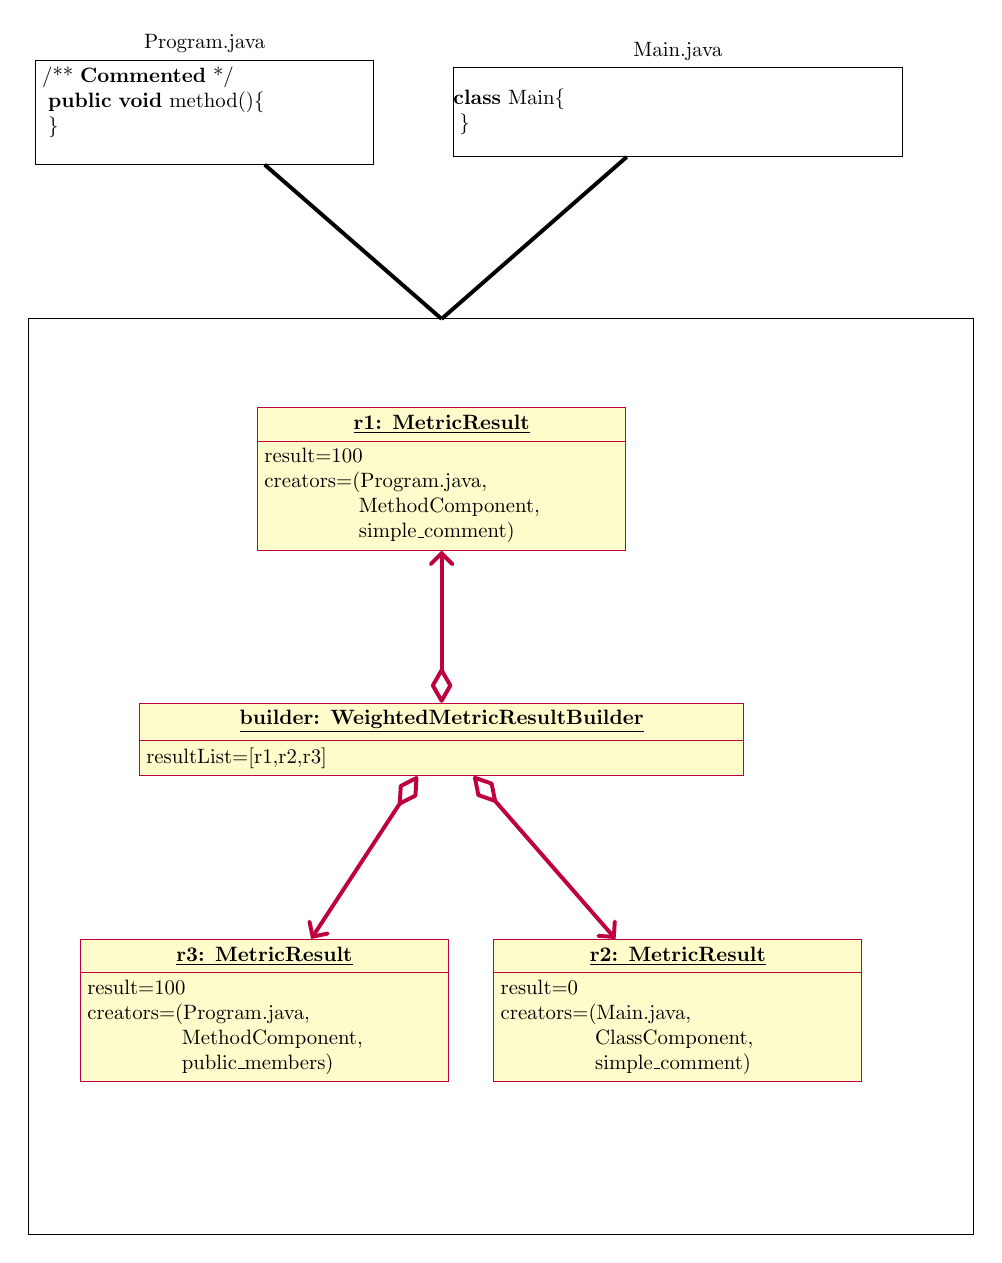
\begin{tikzpicture}[scale=0.75, every node/.style={scale=0.75}]
 \pgfmathsetlengthmacro\breite{6cm}
\pgfmathsetlengthmacro\hoehe{2.567cm}
\pgfmathsetlengthmacro\InnerSep{0.4cm}
\node[draw,
anchor=center, 
inner sep=0pt, 
minimum width=5cm, text width=8cm-\InnerSep,
align=justify,minimum height=1.5cm] (java) {\textbf{class} Main\{\newline 
\hspace*{0.1cm}\}};

\node[draw,text width=5.5cm, left = of java](java2){
/** \textbf{Commented} */ \newline
     \hspace*{0.1cm}\textbf{public} \textbf{void} method()\{\newline
    \hspace*{0.1cm}\}\newline
};
\draw[line width=0.05cm]    (java2) -- (-4,-3.5) ;
\draw [line width=0.05cm](java) -- (-4,-3.5);
\draw[thick,line width=0.05cm] (-4,-3.5) -- (-4,-3.5);

\node[above=-0.0 of java2,line width=0cm]{Program.java};

\node[above=-0.0 of java,line width=0cm]{Main.java};


\draw [] (-11,-3.5) rectangle(5,-19);
\begin{scope} {0,-10}
       \begin{object}[text width=10cm]{builder}{-4,-10}
        \instanceOf{WeightedMetricResultBuilder}
        \attribute{resultList={[r1,r2,r3]}}
      \end{object}
      \begin{object}[text width=6cm]{r1}{-4,-5 }
        \instanceOf{MetricResult}
        \attribute{result=100}
        \attribute{creators=(Program.java,\newline
        \hspace*{1.6cm}MethodComponent, \newline
        \hspace*{1.6cm}simple\_comment)}
      \end{object}
      
        \begin{object}[text width=6cm]{r2}{0,-14 }
        \instanceOf{MetricResult}
        \attribute{result=0}
        \attribute{creators=(Main.java,\newline
        \hspace*{1.6cm}ClassComponent,\newline
        \hspace*{1.6cm}simple\_comment)}
      \end{object}
      
           \begin{object}[text width=6cm]{r3}{-7,-14 }
        \instanceOf{MetricResult}
        \attribute{result=100}
        \attribute{creators=(Program.java,\newline
       \hspace*{1.6cm}MethodComponent,\newline
       \hspace*{1.6cm}public\_members)}
      \end{object}
      

   
\end{scope}
\begin{scope}[line width=0.05cm]
    \aggregation{builder}{}{}{r1}{}{}
    \aggregation{builder}{}{}{r2}{}{}
    \aggregation{builder}{}{}{r3}{}{}

\end{scope}

    
\end{tikzpicture}
     
     \caption{ Veranschaulichung der Bildung eines Gesamtergebnisses}
     \label{fig:metric_weighting}
 \end{figure}
Durch dieses Tupel kann für jedes Teilergebnis die Gewichtung der Metrik, der Komponente und des Dateipfades  abgerufen werden. Durch Multiplikation  aller Gewichtungen entsteht ein Gesamtgewicht.

Abbildung \ref{fig:metric_weighting} veranschaulicht anhand eines vereinfachten Objektdiagramms die Bildung eines Gesamtresultats mittels Gewichtung von verschiedenen Ergebnissen, indem der gewichtete Mittelwert aus Kapitel \ref{chapter:weighted_aggreg} verwendet wird. Hier wird ein hypothetisches Projekt mit zwei Dateien analysiert. Die erste Datei \enquote{Program.java} enthält nur eine öffentliche Methode \textit{method}, was in Java eigentlich nicht möglich ist, aber hier zur Vereinfachung zugelassen sein soll. Die zweite Datei \enquote{Main.java} enthält eine nichtöffentliche Klasse \textit{Main}. In diesem Beispiel werden zwei Metriken verwendet. Die erste Metrik prüft das Vorhandensein der Dokumentation bei allen Komponenten, während die zweite Metrik nur öffentliche Komponenten betrachtet (siehe Kapitel \ref{chapter:metrics_coverage}). In diesem Beispiel soll die Datei \enquote{Main.java} mit dem Faktor $3$ gewichtet werden. Methoden sollen mit dem Faktor $4$ gewichtet werden. Die zweite Metrik \textit{public\_members} wird mit dem Faktor $2$ gewichtet. Alle anderen Dateien, Komponenten und Metriken werden mit dem Standardfaktor $1$ gewichtet.

Das erste Teilergebnis \textit{r1} ist 100, da es die  Methode \textit{method} beschreibt, welche dokumentiert ist. Auch das dritte Teilergebnis \textit{r3} hat den Wert 100, da es die gleiche Komponente nur mit der zweiten Metrik beschreibt. Das zweite Teilergebnis \textit{r2} hat den Wert 0, da es die undokumentierte Klasse \textit{Main} beschreibt.  Es gibt kein weiteres Teilergebnis von \enquote{Main.java}, da die zweite Metrik jegliche nichtöffentliche Komponenten ignoriert. Die Teilergebnisse werden durch den \textit{WeightedMetricResultBuilder} intern gespeichert. 

Das Teilergebnis jeder gefundenen Komponente enthält gemäß dem obigen Vorgehen ein Tupel aus Dateiname, Komponentenname und Metrikname. Beispielsweise enthält das erste  Teilergebnis \textit{r1} das Tupel \enquote{(Program.java, MethodComponent, simple\_comment)}, wobei die einzelnen Bestandteile des Tupels Zeichenketten sind. Basierend auf diesen Informationen kann der \textit{WeightedResultBuilder} eine Gewichtung vornehmen. Das erste Teilergebnis würde mit dem Faktor $1*4*1=4$ gewichtet werden, da es von einer Methode stammt  und ansonsten nicht besonders gewichtet wird. Das zweite Teilergebnis erhält das Gewicht $3*1*1=3$, da es von der Datei \enquote{Main.java} stammt. Zuletzt besitzt das dritte Teilresultat die Gewichtung $1*4*2=2$, da es von der zweiten Metrik berechnet wurde und auch von einer Methode stammt. 

Basierend auf diesen Teilresultaten kann ein Gesamtergebnis berechnet werden. Hierzu wird jedes Ergebnis mit dessen Gewicht multipliziert und anschließend wird durch die Summe der Gewichte geteilt. Bezogen auf das Beispiel würde die Rechnung folgendermaßen aussehen:
\begin{equation}
    \frac{4*100 + 3*0 + 8*100}{4+3+8}=80
\end{equation}
Dieses Ergebnis ist dann Maß für die Bewertung der Dokumentationsqualität dieses hypothetischen Projektes. 










\begingroup
\renewcommand{\cleardoublepage}{} % TODO maybe removing this and next
\renewcommand{\clearpage}{}
\chapter{Umsetzung}\label{chapter:program}
\endgroup
In diesem Kapitel wird auf die Umsetzung der in Kapitel \ref{chapter_conception} beschriebenen Architektur eingegangen. In Kapitel \ref{chapter:tool_running} wird zunächst erläutert, wie das Programm konkret ausgeführt wird, um die Dokumentationsqualität zu ermitteln. Danach wird in Kapitel \ref{chapter:traversing} beschrieben, wie das Programm die einzelnen Java-Dateien findet, damit diese weiterverarbeitet werden können.  Außerdem wird in Kapitel \ref{chapter:antlr4_impl} erläutert, wie ANTLR4 verwendet wird, um Java-Dateien zu parsen. Daraufhin wird erklärt, wie die strukturierten Kommentare geparst werden (Kapitel \ref{chapter:comment_parsing}).  In Kapitel \ref{chapter:conf} wird die Konfiguration des Tools erläutert. Um auch einen Vergleich zwischen den aktuellen und den vorherigen Zustand der Dokumentationsqualität zu ermöglichen, wird in Kapitel \ref{chapter:saving} beschrieben, wie das letzte Ergebnis der Bewertung gespeichert werden kann. In Kapitel \ref{chapter:github_actions_impl} wird erklärt, wie das Programm in GitHub Actions eingebunden wird und wie es so genutzt werden kann. Zum Abschluss werden in Kapitel \ref{chapter:metrics} und \ref{chapter:algos_aggregation} die implementierten Metriken und die implementierten Aggregationsalgorithmen erläutert. 


\hfill
\section{Ausführung des Programms}\label{chapter:tool_running}
In diesem Unterabschnitt wird beschrieben, wie das Programm die in Kapitel \ref{chapter_conception}
beschriebenen Arbeitspakete nutzt, um die Qualität der Softwaredokumentation zu bewerten. 

Die Koordination des Programms wird in der Datei \enquote{index.ts} durchgeführt, die als Einstiegspunkt des Programms verstanden werden kann. In dieser Datei werden die einzelnen Module des Programms in der richtigen Reihenfolge aufgerufen und die Ergebnisse eines Moduls werden durch die \enquote{index.ts}-Datei an das folgende Modul/Arbeitspaket übergeben, soweit sie dort benötigt werden. Dadurch sind die Module voneinander entkoppelt und greifen nicht direkt aufeinander zu. 

Im ersten Schritt  muss die Konfiguration des Programms geladen werden. Dazu wird das Arbeitsverzeichnis von der Kommandozeile gelesen. Basierend auf das Arbeitsverzeichnis kann dann die Konfiguration des Tools geladen werden, wie es in Kapitel \ref{chapter:conf} beschrieben ist.  

Anschließend müssen einige Objekte  initialisiert werden. Hierzu werden die Werte aus der Konfiguration (z.~B. der Konfigurationsdatei) verwendet. Beispielsweise kann durch \textit{builder} der Algorithmus festgelegt werden, der die Einzelergebnisse der einzelnen Metriken zu einem Gesamtresultat kombiniert. Dazu wird eine Fabrikmethode verwendet, da damit die Konstruktion eines Objektes aus einer Zeichenkette möglich ist und somit der Anwender in der Konfiguration nur eine bestimmte Zeichenkette oder ID zur Konstruktion eines komplexeren Objektes angeben muss \cite[S.~149--161]{gamma2015design}. Zudem werden die Metriken, die zur Analyse verwendet werden sollen, durch den Metrikmanager registriert.

Außerdem wird eine assoziative Liste für die Dateien und die Metriken erstellt, die einem eindeutigen Metriknamen bzw. einem Wildcard-Pattern einer Datei ein Gewicht zuordnet. Diese Liste kann einem \textit{WeightResolver} übergeben werden, der wiederum dem  \textit{MetricResultBuilder} übergeben wird. Falls dieser keine Gewichtung benötigt, werden diese Informationen ignoriert. 

Danach müssen die relevanten Dateien gefunden werden. Dazu werden dem Traversierer (siehe Kapitel \ref{chapter:traversing}) die Wildcard-Patterns der zu inkludierenden Dateien und der auszuschließenden Dateien übergeben. Mit der Methode \textit{getRelevantFiles} werden dann alle relevanten Dateien zurückgegeben.

In nächsten Schritt muss jede Datei mit jeder Metrik geprüft werden und die Ergebnisse gesammelt werden. Hierzu wird eine verschachtelte For-Schleife verwendet. Dabei gibt es zwei Möglichkeiten zur Verschachtelung. Im ersten Fall könnte in der äußeren Schleife jede Datei und in der inneren jede Metrik durchlaufen werden. Alternativ könnte auch die innere und äußere Schleife vertauscht werden. Der erste Ansatz hat den Vorteil, dass jede Datei nur einmal geladen werden muss, was einen Geschwindigkeitsvorteil bringen kann, deshalb wird dieses Verfahren auch gewählt. Pro Iteration der inneren Schleife wird die aktuelle Datei von der jeweiligen Metrik analysiert und alle gefundenen Metrikresultate, die von den einzelnen Komponenten der Datei stammen, zu einem \textit{MetricResultBuilder} hinzugefügt.

Nach Abschluss der beiden Schleifen steht das Ergebnis durch Aggregation der Resultate in dem \textit{MetricResultBuilder} zur Verfügung und kann genutzt werden, um die Qualität der Dokumentation mit dem Grenzwert bzw. dem letzten Wert zu vergleichen. Wird bei diesem Vergleich festgestellt, dass die Dokumentationsqualität nicht ausreichend ist, wird eine Ausnahme geworfen und das Programm bricht ab. Wird das Programm mittels GitHub Actions ausgeführt, so kann durch diese Ausnahme ein Merge verhindert werden.

Die Abbildungen \ref{fig:passed} und \ref{fig:absolute} im Anhang \ref{chapter:pictures_tool} visualisieren die Ausgabe des Programmes bei einer ausreichenden bzw. mangelhaften Dokumentationsqualität.

\section{Traversierung aller relevanten Dateien und der Komponenten}\label{chapter:traversing}
Softwareprojekte bestehen aus Hunderten von Dateien, die nicht alle Quellcode enthalten. Beispielsweise gehören Konfigurationsdateien, Ressourcendateien wie Bilder oder binäre Dateien zu den Dateien, bei denen eine Analyse der Softwaredokumentation im Hinblick auf die begrenzte Zeit für die Bachelorarbeit nicht implementierbar ist. Daher ist es sinnvoll, bestimmte Dateien bei der Analyse auszuschließen beziehungsweise nur bestimmte Dateien zu betrachten. Bei einer Weiterentwicklung des Tools nach Abschluss der Bachelorarbeit kann das Tool auf andere Dateitypen ausgeweitet werden, um so ein besseres Gesamtbild über die Softwaredokumentation zu erhalten.

Um die relevanten Dateien zu finden, wird zunächst ein übergeordnetes Verzeichnis benötigt, was bei Softwareprojekten aber der Standard sein sollte. Dieses Verzeichnis kann dann rekursiv durchlaufen werden und somit die Liste aller darin gespeicherten Dateien abgerufen werden. Die relevanten Dateien können dann durch Überprüfung ihres Dateinamens mittels bestimmter Regeln ermittelt werden, die der Benutzer des Tools festlegen kann.

Beim DocEvaluator wird hierzu die NPM-Bibliothek \textit{Minimatch} \cite{Minimatch} verwendet, die es ermöglicht, Dateinamen mit Wildcard-Patterns zu vergleichen. Zum Beispiel könnte der Dateiname \enquote{test.txt} mit der Wildcard \enquote{test.*} verglichen werden und die Bibliothek würde eine Übereinstimmung melden.

Auch die Komponenten einer Datei müssen traversiert werden, damit bei jeder Komponente die Dokumentation überprüft werden kann. Da die Komponenten wie in Kapitel \ref{chapter:parsing} beschrieben rekursiv aufgebaut sind, kann dies mittels einer Tiefensuche durchgeführt werden.

\subsubsection{Ignorieren bestimmter Kommentare}

Unter Umständen kann es sinnvoll sein, bestimmte Komponenten bei der Bewertung auszulassen, weil sie beispielsweise noch nicht vollständig implementiert sind, in einer nicht-englischen Sprache dokumentiert sind oder ein anderer gewichtiger Grund existiert. Für diesen Fall kann die allgemeine Beschreibung der Dokumentation einer Komponente  den Begriff \enquote{\%ignore\_this\%} oder \enquote{\%ignore\_node\%} enthalten. Bei Ersterem wird nur diese Komponente ignoriert und als nicht existent betrachtet. Bei Zweiterem werden sowohl diese Komponente als auch alle Kinder dieser Komponente ignoriert, sofern sie existieren.




\section{Implementierung von ANTLR4 für Java}\label{chapter:antlr4_impl}

Für die Programmiersprache Java steht eine ANTLR4-Grammatik, die auf GitHub unter der BSD-Lizenz angeboten wird, zur Verfügung \cite{ANTLRgrammarforjava}, allerdings ignoriert diese Grammatik alle Kommentare. Daher müssen einige Änderungen sowohl am Lexer als auch am Parser vorgenommen werden. Im Lexer werden standardmäßig alle Tokens aus einem Kommentar in einem versteckten Kanal gespeichert, was dazu führt, dass diese Tokens vom Parser ignoriert werden. Um dieses Problem zu lösen, wird das Verhalten durch Definition eines neuen Tokens so geändert, dass Javadoc-Kommentare auch vom Parser verarbeitet werden können, aber mehrzeilige und einzeilige Kommentare weiterhin ignoriert werden. Einzeilige Kommentare sind hier nicht relevant, da sie kein Javadoc enthalten.

Mehrzeilige Kommentare könnten theoretisch auch berücksichtigt werden, da einige Entwickler diese anstelle von Javadoc benutzen. Allerdings werden solche mehrzeiligen Kommentare vor Komponenten nicht von Tools erkannt und haben daher einen geringeren, aber durchaus vorhandenen Nutzen \cite[S.~4]{HowDocumentationEvolvesoverTime}. Deshalb werden Komponenten, die zwar mit mehrzeiligen Kommentaren, aber nicht mit Javadoc dokumentiert sind, wie undokumentierte Komponenten betrachtet. Für einen Entwickler sollte es so schnell möglich sein, solche nicht korrekt dokumentierten Komponenten zu identifizieren und deren mehrzeilige Kommentare in gültige Javadoc-Kommentare umzuwandeln und so die Qualität der Dokumentation zu erhöhen. Für andere Programmiersprachen können jedoch normale mehrzeilige wie strukturierte Kommentare betrachtet werden, wenn dies für sinnvollerer erachtet wird.

Mehr Änderungen müssen an der entsprechenden Parser-Datei \enquote{JavaParser.g4} durchgeführt werden.  Da diese Änderungen für die eigentliche Thematik dieser Bachelorarbeit nur eine untergeordnete Rolle spielen, wird hier nicht jede Änderung genauer erklärt. Tabelle \ref{tab:parser_changes} im Anhang \ref{chapter:appendix_parser_changes} listet alle Änderungen an der Parserdatei auf. Die geänderte Parserdatei und das Original befinden sich auch im digitalen Anhang im Verzeichnis \enquote{parser\_changes}. 

Um die Informationen aus einer Java-Datei mittels ANTLR4 zu verarbeiten, kann das Visitor-Pattern verwendet werden \cite[S.~400ff.]{gamma2015design}. Mit einem Visitor kann die Baumstruktur, die ANTLR4 erstellt hat, traversiert werden, damit so nur die notwendigen Informationen herausgefiltert werden. Andere Informationen (wie z.~B. Conditional-Branches) können so ignoriert werden.  
		\begin{figure} [htbp!]
			\lstinputlisting
			[caption={Codeauschnitt aus  Methoden-Visitor},
			label={lst:visit_method_example},
			captionpos=b,language=javascript, basicstyle=\footnotesize, tabsize=2, showstringspaces=false,  numbers=left]
			{figures/chapter4/visit_method_example.js}
		\end{figure}
Listing \ref{lst:visit_method_example} zeigt einen Ausschnitt vom Visitor für Methodendeklarationen aus dem Quellcode des Tools. Hier ist die Baumstruktur leicht sichtbar. Alle Einzelbestandteile einer Methode wie z. B. Bezeichner, Rückgabetyp etc. sind Kindknoten des \textit{RuleContext} und können über die Methode \textit{getChild} abgerufen werden. So werden sowohl der Bezeichner als auch der Rückgabetyp direkt als Text abgerufen. Diese  beiden Bestandteile bestehen wiederum auch aus weiteren Kindknoten, doch eine weitergehende Betrachtung ist nicht nötig, da nur die Bezeichnung als Zeichenkette benötigt wird. Andere Bestandteile wie die Methodenparameter sind jedoch komplexer, deswegen werden sie von separaten Visitors betrachtet.

\section{Parsen der strukturierten Kommentare}\label{chapter:comment_parsing}
Um die strukturierten Kommentare in das Format nach Kapitel \ref{chapter:structured_comments} zu bringen, wird eine simple Heuristik verwendet. Es werden so viele Zeilen als allgemeine Beschreibung betrachtet, bis eine Zeile auftaucht, die mit einem Tag wie z.~B. \enquote{@param} beginnt, der den allgemeinen Teil beendet.

Anschließend werden diese Tags verarbeitet. Benötigt ein Tag einen Parameter, so wird die Zeile in drei Teilen an den Leerzeichen aufgetrennt. Dabei ist der erste Teil der Typ des Tags, der zweite Teil der Parameter und der Rest (mit allen übrigen Leerzeichen) die Beschreibung des Tags.
Bei einem Tag ohne Parameter wird die Zeile in zwei Teile getrennt, wobei hier der erste Teil der Typ des Tags und der letzte Teil die Beschreibung ist.

Diese Heuristik sollte die gängigsten Javadoc-Blöcke verarbeiten können. Alternativ könnte auch ANTLR4 Javadoc parsen. Allerdings ist dies aufgrund der Mischung von natürlicher Sprache und der relativen Flexibilität von Javadoc nicht trivial und wird daher nicht implementiert. 



\section{Konfiguration des Tools}\label{chapter:conf}
Zur Nutzung des Tools werden bestimmte Informationen benötigt, die aus verschiedenen Quellen bezogen werden. Zunächst benötigt das Tool den Pfad, der die Quelldateien enthält, die nach Kapitel \ref{chapter:traversing} traversiert werden sollen. Dieser wird als namenloser Parameter über die Kommandozeile übergeben. Er ist optional, da bei dessen Fehlen das aktuelle Arbeitsverzeichnis genommen wird. Die weiteren Informationen werden aus zwei Quellen bezogen. Wenn beide Quellen fehlen, werden Standardwerte genommen. Die erste Quelle ist eine \ac{JSON}-Datei namens \mbox{\enquote{comment\_conf.json}}, welche die notwendigen Daten für die Arbeit des Programms enthält. Listing \ref{lst:example_conf} zeigt eine beispielhafte Konfigurationsdatei im \ac{JSON}-Format.

\begin{figure}[htbp]
\lstinputlisting
[caption={Beispielhafte Konfigurationsdatei für das Tool},
label={lst:example_conf},
captionpos=b, basicstyle=\footnotesize, tabsize=2, showstringspaces=false,  numbers=left,language=JSON]
{figures/chapter4/example_conf.json}
\end{figure}

In dieser Beispieldatei  werden alle Dateien mit der Dateiendung \enquote{.java} bei der Traversierung betrachtet (Z. 1). Außerdem werden dabei keine Dateien bei der Traversierung ausgeschlossen (Z. 2). Diese beiden Werte entsprechend dabei ihre Standardwerte. Sie könnten also bei dieser Konfigurationsdatei weggelassen werden und das Programmverhalten würde sich nicht ändern.

Anschließend (Z. 4--11) werden die zu verwendenden Metriken definiert. Jede Metrik besitzt einen \textit{metric\_name}, der den Typ der Metrik spezifiziert. In Zeile 6 wäre dies beispielhaft die Metrik \enquote{Anteil der dokumentierten Komponenten an allen Komponenten} (vgl. Kapitel \ref{chapter:metrics_coverage}). Anhang  \ref{appendix_metrics} beschreibt alle implementierten Metriken mit ihren Namen. Diese Namen werden vom Metrikmanager dazu genutzt, um die passende Klasse zu finden und so ein Metrikobjekt zu erzeugen. Außerdem erhält jede Metrik durch \textit{unique\_name} einen eindeutigen Namen (hier z.~B. \enquote{m1}). Dieser kann auch weggelassen werden. Dann wird der eindeutige Name aus dem Namen der Metrik und einer fortlaufenden Nummerierung erzeugt. Zudem besitzt jede Metrik das Attribut \textit{weight}, welches zur Bestimmung der Relevanz bzw. des Gewichts der Metrik dient und von einem \textit{MetricResultBuilder} zur Bestimmung eines Gesamtergebnisses benutzt werden kann. Ein \textit{MetricResultBuilder}, der keine Gewichtung der Metriken benötigt, wird diese Information ignorieren. Das Gewicht ist ebenfalls optional. Bei dessen Fehlen wird das Gewicht \enquote{1} eingesetzt.  Durch \textit{params}  werden der Metrik die Parameter übergeben, die sie benötigt. Die genaue Anzahl und Struktur der Parameter hängen von der jeweiligen Metrik ab. Fehlen diese Parameter, so werden standardmäßige Parameter verwendet.

Fehlt der Eintrag \enquote{metrics}, so werden alle implementierten Metriken mit ihren Standardwerten genommen.

Als Nächstes (Z. 12) wird der Schwellwert festgelegt. Dieser Wert legt fest, ob das Programm beim Unterschreiten dieses Wertes mit einer Fehlermeldung abbrechen soll. In Zeile 13 wird der \textit{MetricResultBuilder} festgelegt, der bestimmt, wie die Einzelergebnisse aggregiert werden. In dem Beispiel werden alle Teilresultate mittels eines gewichteten Mittelwertes zu einem Gesamtergebnis aggregiert.  In Zeile 14 wird durch \mbox{\textit{ relative\_threshold }} festgelegt, um wie viel sich die Dokumentationsqualität verschlechtern muss, damit ebenfalls eine Fehlermeldung erscheint. Dies wird in Kapitel \ref{chapter:saving} genauer erläutert.



\bigskip
Die zweite Quelle für die Informationen sind die Eingabeparameter aus GitHub Actions. Dazu wird, wie in Kapitel \ref{chapter:github_actions_impl} beschrieben, jeder Parameter aus der \ac{JSON}-Datei auch in der \enquote{action.yml}-Datei übernommen. Bei der Ausführung des Programms stehen diese Eingabedaten über Umgebungsvariablen bereit. Jede Umgebungsvariable beginnt mit der Zeichenkette \enquote{INPUT\_}, anschließend folgt der Name des entsprechenden Parameters (wie in der \ac{JSON}-Datei), wobei der Name allerdings komplett in Großbuchstaben geschrieben ist. So steht  \enquote{absolute\_threshold} als \enquote{INPUT\_ABSOLUTE\_THRESHOLD} zur Verfügung.

Da es durchaus sein kann, dass sowohl eine Konfigurationsdatei existiert als auch die Umgebungsvariablen gesetzt sind, muss klar festgelegt werden, welcher Wert eines Parameters am Ende genommen wird. Bei dem Tool haben die von GitHub Actions erzeugten Umgebungsvariablen  Vorrang, da das Tool für die Verwendung in GitHub Actions konzipiert wurde.  Die Auflistung im Anhang \ref{enum:tool_javadoc_conf} listet alle Parameter des Tools nochmals auf und erläutert sie zusätzlich. 

\begin{comment}
Das Tool \textit{create\_conf}, das im Hauptverzeichnis im GitHub-Repository liegt kann eine beispielhafte Konfigurationsdatei erstellen, indem \textit{node create\_conf.js --out PATH --type json} aufgerufen wird. Dabei ist \textit{PATH} ein Pfad ohne Dateiname. Dieses Hilfstool legt dann eine Konfigurationsdatei namens \enquote{comment\_conf.json} in dem angegebenen Verzeichnis an. 
\end{comment}
\section{Speicherung des letzten Ergebnisses}\label{chapter:saving}
Neben der bereits erwähnten Möglichkeit, einen absoluten Grenzwert für die Dokumentationsqualität zu definieren, ist auch ein inkrementeller Vergleich interessant. Dabei wird das Ergebnis der Dokumentationsqualität zwischengespeichert. Bei einem neuen Start des Tools kann das alte Ergebnis mit dem neuen Ergebnis verglichen werden. Verschlechtert sich das Ergebnis über einen gewissen Schwellwert hinaus, so sollte der Entwickler ebenfalls gewarnt werden, selbst wenn die Dokumentationsqualität noch über der absoluten Grenze liegt. Schließlich kann dies ein Trend sein, der zum baldigen Unterschreiten des absoluten Grenzwertes führen kann. 

Der Ort zur Speicherung des letzten Wertes ist dabei flexibel. Standardmäßig wird der Wert in einer Datei namens \enquote{.evaluator\_last\_state.txt} gespeichert. Falls das Programm im Kontext von GitHub Actions ausgeführt wird, sollte allerdings beachtet werden, dass diese Datei nach der Beendigung des Workflows gelöscht wird. Dieses Problem kann dadurch gelöst werden, dass die geänderte Datei im Repository des zu analysierenden Projektes hochgeladen wird. Dies kann beispielsweise mit dem Tool \textit{Add \& Commit} \cite{add_commit} erledigt werden. Nachteilhaft ist an diesem Vorgehen allerdings, dass hierdurch in dem Commit-Verlauf automatisierte Commits erscheinen, sodass der Überblick verloren gehen kann.  Eine weitere Möglichkeit zur Speicherung des Wertes wäre es, den Wert an einen externen Server zu senden und bei einem erneuten Start diesen Wert abzurufen. 

  
\section{Einbindung in GitHub Actions}\label{chapter:github_actions_impl}
Um das Tool in GitHub Actions einzubinden, müssen einige Schritte erfolgen. Zunächst muss eine \enquote{action.yaml} geschrieben werden, die das GitHub-Repository als Aktion markiert und die notwendigen Befehle für die Ausführung enthält. Listing  \ref{lst:action} zeigt einen beispielhaften Code der Action. Zur Übersichtlichkeit wird in diesem Listing nur ein Eingabeparameter definiert. Die restlichen Eingabeparameter werden im Programm analog definiert.
\begin{figure} [htbp]
\lstinputlisting
[caption={Beispielhafte Action-Datei für das Tool},
label={lst:action},
captionpos=b, basicstyle=\footnotesize, tabsize=2, showstringspaces=false,  numbers=left,language=YAML]
{figures/chapter4/action.yml}
\end{figure}

In den ersten beiden Zeilen werden Attribute wie der Name und eine Beschreibung gesetzt. Danach (Z. 4--7) wird der Eingabeparameter für die minimal erlaubte Bewertung für die Dokumentationsqualität definiert, damit dieser von den Nutzern der Aktion verändert werden kann. In den Zeilen 8 bis 10 ist der wichtige Programmcode enthalten, in denen die Aktion als JavaScript-Aktion mit der Node-Version 16 festgelegt wird. Zudem enthält die letzte Zeile auch den Pfad zur Quellcodedatei, mit dem das Programm gestartet werden soll. 

\bigskip
Eine JavaScript-Aktion in GitHub Actions benötigt JavaScript, sodass der TypeScript-Code des Tools erst in JavaScript umgewandelt werden muss. Damit das Programm bei der Veröffentlichung einer neuen Version in einen auslieferbaren Zustand gebracht werden kann, wird ein weiterer Workflow benötigt, der bei jedem Push in dem Main-Zweig folgende Schritte ausführt:
\begin{enumerate}
    \item Klonen des Main-Branch des Repositorys (wie bei den meisten anderen Workflows)
    \item Aufruf von TSC, Konvertierung des TypeScript-Codes in JavaScript
    \item Aufruf und Benutzung von \textit{NCC} \cite{ncc}. Packen aller JavaScript-Dateien in einer einzigen Datei
    \item Kopieren der generierten Datei, die den gesamten Quellcode enthält, und der \enquote{action.yml}, in eine (neue) Branch \textit{action}. Dies wird mittels der Aktion \textit{Branch-Push} \cite{Branch-Push} durchgeführt
\end{enumerate}
Durch diese Schritte wird eine neue Branch erstellt, die nur die notwendige JavaScript-Datei und die \textit{action.yml} enthält. Dadurch können Nutzer der Aktion diese schneller herunterladen und nutzen. Es wäre auch möglich, kein \textit{NCC} zu verwenden, also alle Javascript-Dateien in die neue Branch zu kopieren, allerdings ist die hier gewählte Methode praktikabler, da dann nur ein Lesezugriff beim Starten des Programms erforderlich ist und so ein Geschwindigkeitsvorteil existiert. 

\subsubsection{Nutzung der Aktion}

Die oben erstellte Aktion kann nun von jedem GitHub-Repository verwendet werden. Dazu kann das folgende Listing \ref{lst:action_using} als zusätzlicher Schritt in einem Workflow eingebunden werden. 
\begin{figure} [htbp]
\lstinputlisting
[caption={Verwendung der Aktion in einem Workflow},
label={lst:action_using},
captionpos=b, basicstyle=\footnotesize, tabsize=2, showstringspaces=false,  numbers=left,language=YAML]
{figures/chapter4/action_using.yml}
\end{figure}

Hier wird die aktuelle Version des DocEvaluators aus der Branch \textit{action} heruntergeladen und automatisch ausgeführt. Als Parameter wird beispielsweise ein Grenzwert von 20 übergeben, der jedoch nach Belieben angepasst werden kann. Wenn das entsprechende Ereignis des Workflows eintritt (z. B. ein Push-Ereignis), wird der DocEvaluator mit diesem Parameter aufgerufen und zeigt unter der Registerkarte \textit{Actions} eine Fehlermeldung an, wenn die Dokumentationsqualität den Grenzwert unterschreitet und somit nicht ausreichend ist.
\begin{comment}
Das Tool \textit{create\_conf}, das im Hauptverzeichnis im GitHub-Repository liegt, kann ein Workflow erstellen, indem \textit{node create\_conf.js --out PATH --type yaml} aufgerufen wird. Dieses kleine Hilfstool erzeugt dann ein beispielhafter Workflow mit allen Eingaben in dem angegebenen Pfad, um es leicht in GitHub einzubinden.
\end{comment}

%\documentclass[a4paper,12pt,oneside, bibliography=totoc]
{scrbook}
\usepackage[utf8]{inputenc}
\usepackage{pgf-umlcd}
% Schrift und -kodierung
\usepackage[T1]{fontenc}
\usepackage{lmodern}
\usepackage{tcolorbox}
% Sprache/Silbentrennung
\usepackage[english]{babel} %TODO change to german if desired
\usepackage{booktabs}
\usepackage{amsmath}
\usepackage{floatflt}
\usepackage{float} 
\usepackage{verbatim}
\usepackage{hyperref}
\usepackage{graphicx}
\usepackage{pbox}
\usepackage{algorithmic}
\usepackage{algorithm}
\usepackage{subcaption}
\usepackage{siunitx}
\usepackage[autostyle]{csquotes}
\usepackage{todonotes}
\usepackage{svg}
\usepackage[page, title, titletoc, header]{appendix} %prettier appendix

\svgpath{{../figures/}}

\usepackage[printonlyused]{acronym}
\usepackage{listings} 
%\usepackage{subfig}
\lstset{xleftmargin=2em} %Proper indention of listings

\widowpenalty10000
\clubpenalty10000
\usepackage{tabularx} %For tables
\usepackage{csquotes} %For Quotes





%Footnote Numbering not reset in new chapters
\usepackage{chngcntr}
\counterwithout{footnote}{chapter}


%Remove last point after section/subsections
\renewcommand{\autodot}{}

\usepackage[htt]{hyphenat} %damit texttt noch Linebreaks mit Silbentrennung erzeugt
\newcommand{\code}[1]{\texttt{#1}} %Programmcode im Textfluss in passendem Font ausgeben

%Literatur
%Ordering in references checken, vermutlich was mit style=numeric zu tun
\usepackage[
   backend=biber,
   sorting= none,
   giveninits=true,
   date=long,
   urldate=long,
   url=false
]{biblatex}
\addbibresource{database.bib}
%\addbibresource{literatur2.bib}


\usepackage[]{hyperref}

\begin{document}
\frontmatter %roman page numbers





	\titlehead{
	\begin{center}
	   \includegraphics[width=10cm]{figures/unilogo.pdf}\\
	   	Institute of Computer Science, Software Engineering Group
	\end{center}
	}
	\subject{Master Thesis: }
	\title{ Refactoring data clumps with the help of ChatGPT
 }
	\author{Timo Schoemaker\\ Immatriculation number: 978621} %engl. Matriculation Number

	\date{\today\\
	Advisor: Prof. Dr.-Ing. Elke Pulvermüller \\ %Deutsch: Erstebetreuer
	Co-Advisor: Nils Baumgartner, M. Sc.} %Deutsch: Zweitbetreuer
	
	\maketitle
	
	\clearpage
	
	\addchap*{Abstract}
\textbf{Deutsch}

Code-Smells (z.~dt. übelriechender Code ) gelten als zuverlässiges Anzeichen für Quellcode mit Qualitätsprobleme, was zu höheren Wartungskosten führt. Refaktorisierungen von Code-Smells können diese Probleme lösen, haben aber in der Praxis nur eine geringe Priorität. Eine Lösung können automatisierte Refaktorisierungen sein, die den Entwickler bei der Behebung unterstützen. Der Fokus dieser Masterarbeit wird auf das Code-Smell „data clump“ (z.~dt. Datenklumpen) liegen, bei dem Variablen im Quellcode dupliziert werden. Bislang gibt es noch keine automatisierten Werkzeuge zur Behebung dieses Code-Smells. Mithilfe von Sprachmodellen wie ChatGPT, die  seit einiger Zeit große Aufmerksamkeit erregt haben,  wird ein modulares Werkzeug entwickelt, das die Detektion und Behebung von Data-Clumps automatisch durchführen kann.  Die Eignung von ChatGPT für diese Aufgabe wird  anschließend mittels einer Umfrage auf GitHub und anderen Experimenten untersucht. 
%\linebreak
\bigskip

\noindent
%\bigskip
\textbf{English} 
The existence of code smells is a reliable indicator for code quality issues which often induces higher maintenance costs. Refactoring code smells is an effective way to improve the quality of the code, but is not the priority of many developers.  Therefore, automatic refactoring tools can help to support developers to fix code smells. This master thesis focuses on one particular code  smell named data clumps, which is the duplication of variables across the code. No automatic refactoring tool for this code smell exists. Employing the capabilities of large language models such as ChatGPT that  recently have gained widespread attention, a modular tool is developed  that automatically detects and fixes data clumps. The thesis evaluates whether ChatGPT is suitable for this task via a GitHub pull request survey and other experiments. 




	\clearpage
	
	\tableofcontents
	\clearpage

	




\lstdefinelanguage{YAML}{
  morekeywords=
  {
    name:,on:,jobs:,steps:,uses:,run:,echo,workflow_dispatch:,description:,inputs:,required:,default:,runs-on:,using:,main:,with:,author:, absolute_threshold:
  },
  keywordstyle=\color{black}\bfseries,
  ndkeywords={false,compf/JavaDocEvaluator@action},
  ndkeywordstyle=\color{black}\bfseries,
  identifierstyle=\color{black},
  sensitive=false,
  comment=[l]{//},
  morecomment=[s]{/*}{*/},
  commentstyle=\color{purple}\ttfamily,
  %stringstyle=\color{red}\ttfamily,
  morestring=[b]',
  morestring=[b]",
  alsodigit={:},
  alsoletter={/,@,-}
}




\lstdefinelanguage{ANTLR}{
  keywords=
  {
   formalParameter:,variableModifier:,typeType:,variableDeclaratorId:,JCOMMENT:
  },
  keywordstyle=\color{black}\itshape,
  identifierstyle=\color{black},
  sensitive=false,
  comment=[l]{//},
  morecomment=[s]{/*}{*/},
  commentstyle=\color{purple}\ttfamily,
  morestring=[b]',
  morestring=[b]",
  alsodigit={:},
}

\lstdefinelanguage{JSON}{
    tabsize             = 4,
    showstringspaces    = false,
    keywords            = {false,true,include,exclude,metrics,metric_name,weight,unique_name,params,absolute_threshold,builder,relative_threshold},
    alsoletter          = 0123456789.*,
    ndkeywordstyle         = \color{red},
  keywordstyle=\color{black}\bfseries,
}





\lstdefinelanguage{javascript}{
  keywords={typeof, new, true, false, catch, function, return, null, catch, switch, var, if, in, while, do, else, case, break,let,this,private},
  keywordstyle=\color{black}\bfseries,
  identifierstyle=\color{black},
  sensitive=true,
  comment=[l]{//},
  morecomment=[s]{/*}{*/},
  commentstyle=\color{purple}\ttfamily,
  stringstyle=\color{red}\ttfamily,
  morestring=[b]',
  morestring=[b]",
}
%\ac{Abk.}         % fügt die Abkürzung ein, außer beim ersten Aufruf, hier wird die Erklärung mit angefügt
%\acs{Abk.}        % fügt die Abkürzung ein
%\acf{Abk.}        % fügt die Abkürzung UND die Erklärung ein
%\acl{Abk.}        % fügt nur die Erklärung ein

%\chapter*{Acronyms}
\addchap{Abkürzungsverzeichnis}

%%%%%%%%%%%%%%%%%%%%%%%
\begin{acronym}[E/E/PE] %sorgt fuer proper indention
	\acro{API}{\emph{Application Programming Interface}}
	\acro{AST}{\emph{Abstract Syntax Tree}}
	\acro{ATL}{\emph{Atlas Transformation Language}}
	\acro{BMWi}{\emph{Bundesministerium für Wirtschaft und Energie}}
	\acro{CIM}{\emph{Computation-Independent Model}}
	\acro{CDC}{\emph{Code-level design choice}}
	\acro{CR}{\emph{Code-level requirement}}
	\acro{CI/CD}{\emph{Continuous Integration/Continuous Delivery}}
	\acro{CRC}{\emph{Cycling Redundancy Checks}}
	\acro{E/E/PE}{\emph{Electrical/Electronic/Programmable Electronic}}
	\acro{ECC}{\emph{Error Detecting and Correcting Codes}} 
	\acro{EMF}{\emph{Eclipse Modeling Framework}}
	\acro{EGL}{\emph{Epsilon Generation Language}}
	\acro{EOL}{\emph{Epsilon Object Language}}
		\acro{HTML}{\emph{Hyper Text Markup Language}}
	\acro{Epsilon}{\emph{Extensible Platform of Integrated Languages for mOdel maNagement}}
	\acro{FS}{\emph{Functional Safety}}
	\acro{HAL}{\emph{Hardware Abstraction Layer}}
	\acro{HolMES}{\emph{Holistische Modell-getriebene Entwicklung für Eingebettete Systeme unter Berücksichtigung unterschiedlicher Hardware-Architekturen}}
	\acro{IDE}{\emph{Integrated Development Environment}}
	\acro{JSON}{\emph{JavaScript Object Notation}}
	\acro{JDT}{\emph{Java Development Tools}}
	
	\acro{LOC}{\emph{Lines of Code}}
 	\acro{LM}{\emph{Language Model}}

	\acro{MISRA}{\emph{Motor Industry Software Reliability Association}}
	\acro{MBU}{\emph{Multi Bit Upset}}
	\acro{MDA}{\emph{Model Driven Architecture}}
	\acro{MDC}{\emph{Model-level design choice}}
	\acro{MDD}{\emph{Model Driven Development}}
	\acro{MDE}{\emph{Model Driven Engineering}}
	\acro{MOF}{\emph{Meta Object Facility}}
	\acro{MR}{\emph{Model-level requirement}}
	\acro{NLP}{\emph{Natural Language Processing}}
	\acro{OCL}{\emph{Object Constraint Language}}
	\acro{OMG}{\emph{Object Management Group}}
	\acro{PIM}{\emph{Platform-Independent Model}}
	\acro{PSM}{\emph{Platform-Specific Model}}
	\acro{SER}{\emph{Soft Error Rate}}
	\acro{SEU}{\emph{Single Event Upset}}
	\acro{TMR}{\emph{Triple Modular Redundancy}}
	\acro{UML}{\emph{Unified Modeling Language}}
	


%\acro{cMOF}{\emph{complete MOF}}
%\acro{eMOF}{\emph{essential MOF}}

%	\acro{ETL}{\emph{Epsilon Transformation Language}}
%	\acro{EWL}{\emph{Epsilon Wizard Language}}

	
\end{acronym} %See inside for usage of acronmys
\mainmatter %switch roman auf arabic page numbers



\chapter{Introduction}
\setcounter{page}{1} %Seitenzahlen hier mit 1 anfangen

	%Include text from other files into the document --> great for structuring
	\label{sec:introduction}

Ein wichtiger Bestandteil der Softwareentwicklung von heute ist die Softwaredokumentation. Dies liegt unter anderem daran, dass die Größe von Softwareprojekten steigt, sodass die Entwickler schnell den Überblick über das Projekt verlieren können und daher zusätzliche Informationen neben dem Code benötigen \cite[S.~1]{StaticAnalysis:AnIntroduction:TheFundamentalChallengeofSoftwareEngineeringisOneofComplexity.}. Nichtsdestotrotz wird die Softwaredokumentation von Entwicklern oft vernachlässigt \cite[S.~83]{Qualityanalysisofsourcecodecomments}.  Die Gründe für schlechte Dokumentation sind vielfältig. Das Schreiben der Dokumentation wird oft als mühevoll empfunden und erfordert Fähigkeiten, die ein Programmierer nicht zwangsläufig besitzt \cite[S.~70]{AutomaticQualityAssessmentofSourceCodeComments:TheJavadocMiner} \cite[S.~593]{Softwareengineeringandsoftwaredocumentation:aunifiedlongcourse}.  

Weitere Studien verdeutlichen die Problematik der mangelhaften Softwaredokumentation. So belegt eine Umfrage aus dem Jahr 2002 mit 48 Teilnehmern  beispielsweise, dass die Dokumentation  bei Änderungen am System  nur mit Verzögerung angepasst wird. Knapp 70~\% der Teilnehmer stimmen der Aussage zu, dass die Dokumentation immer veraltet ist.   \cite[S.~28--29]{TheRelevanceofSoftwareDocumentationToolsandTechnologies:ASurvey}

Eine weitere Studie  \cite[S.~1199--1208]{SoftwareDocumentationIssuesUnveiled} aus dem Jahr 2019 verdeutlicht viele Aspekte aus der vorgenannten Umfrage. Es wurden dabei Daten aus Stack Overflow, GitHub-Issues, Pull-Requests und Mailing-Listen automatisiert heruntergeladen und dann von den Autoren analysiert, ob und inwieweit diese durch mangelhafte Softwaredokumentation verursacht wurden.  Die Studie belegt, dass von 824 Problemen, die etwas mit dem Thema \enquote{Softwaredokumentation} zu tun haben, 485 sich auf den Inhalt der Dokumentation beziehen (wie z.~B. unvollständige, veraltete oder sogar inkorrekte Dokumentation). Bei 255 Einträgen gab es Probleme mit der Struktur der Dokumentation, sodass beispielsweise Informationen schlecht auffindbar sind oder nicht gut verständlich sind.


Eine andere Umfrage aus dem Jahr 2014 mit 88 Teilnehmern zeigt, dass eine automatisierte Überprüfung der Dokumentationsqualität von knapp der Hälfte der befragten Entwickler gewünscht wird. Die Autoren der Studie sehen dies als Zeichen dafür, dass ein grundsätzliches Bedürfnis zur automatisierten Bewertung von Dokumentationen besteht und daher weitere Studien notwendig sind. \cite[S.~340]{TheValueofSoftwareDocumentationQuality}

Die mangelhafte Dokumentation führt dazu, dass nicht nur nachfolgende Entwickler Probleme mit dem Codeverständnis haben, sondern auch Entwickler eines Moduls nach einer längeren Pause Zeit aufbringen müssen, um den Code wieder zu verstehen \cite[S.~511]{vestdam}.  Auch für Kunden/Auftraggeber ist eine gute Dokumentation wichtig, da gut dokumentierte Software tendenziell besser wartbar ist und somit mehr Nutzen bringt \cite[S.~83]{Qualityanalysisofsourcecodecomments} \cite[S.~1]{SoftwareDocumentationManagementIssuesandPractices:ASurvey}.



\section{Zielsetzung}
Aufgrund der Relevanz von gut dokumentierter Software ist eine regelmäßige Rückmeldung über die Dokumentation von hoher Bedeutung. Spezielle Metriken, die eine numerische Auskunft über die Qualität der Softwaredokumentation liefern, sind eine Möglichkeit, diese Rückmeldung zu geben. Diese Metriken verschaffen dem Programmierer eine Einschätzung darüber, ob die Softwaredokumentation ausreichend ist oder eine Verbesserung sinnvoll wäre. Die Qualität der Softwaredokumentation kann auf unterschiedliche Art und Weise bewertet werden. So kann beispielsweise die bloße Existenz einer Dokumentation geprüft werden oder aber auch die Verständlichkeit der Dokumentation bewertet werden, daher kann es sinnvoll sein, mehrere Metriken zu verwenden \cite[S.~29]{pfleeger1992using}. Damit ein Entwickler einen Gesamtüberblick über die Dokumentationsqualität erhält, können diese Metriken kombiniert werden, um eine einzelne numerische Bewertung der Qualität der Dokumentation zu erhalten. 
Dabei ist es auch ratsam, die Metriken zu gewichten oder eine andere Methode zur Kombination der Metrikergebnisse zu benutzen, weil nicht jede Metrik die gleiche Zuverlässigkeit und Relevanz besitzt \cite[S.~1117ff.]{Softwarequalitymetricsaggregationinindustry}.

Damit das Feedback über die Softwaredokumentation auch wahrgenommen wird, sollte die Qualität regelmäßig  überprüft werden. Dies kann automatisiert im \ac{CI/CD}-Prozess erfolgen, bei dem Software kontinuierlich getestet und für den Release (z.~dt. Veröffentlichung) vorbereitet werden kann. Durch CI/CD können Unternehmen effizienter und besser Software entwickeln. So konnte das Unternehmen \textit{ING NL} die gelieferten Function-Points vervierfachen und die Kosten für einen Function-Point auf einen Drittel reduzieren \cite[S.~520]{Vassallo2016}.

\hfill

Basierend auf diesen Überlegungen soll ein Tool (z.~dt. Werkzeug) entwickelt werden. Dieses Tool (im Folgenden auch \textit{DocEvaluator} soll ein gegebenes Software-Projekt analysieren und eine numerische Bewertung abgeben, die eine heuristische Aussage über die Qualität der Softwaredokumentation trifft.  Dabei soll das Tool primär für Javadoc und Java bis Version 8 konzipiert werden, allerdings soll während der Entwicklung auch darauf geachtet werden, dass eine Portierung auf eine andere Programmiersprache ermöglicht wird und die Bewertung der Dokumentation unabhängig von der Programmiersprache funktioniert. Außerdem wird zur Vereinfachung nur englischsprachige Dokumentationen betrachtet. Komplexe \ac{NLP}-Metriken sollen dabei außer Acht gelassen werden. Auch Verfahren, die  den  Quellcode mit der Dokumentation vergleichen, wie z.~B. \textit{iComment} in \cite[S.~145ff.]{icomment}, sollen unberücksichtigt bleiben, da sie im Rahmen dieser Bachelorarbeit zu komplex sind. 

Dabei sollte es nicht unbedingt das Ziel sein, dass jede Komponente dokumentiert ist, sondern dass die wichtigen Komponenten eine gute Dokumentationsqualität haben und somit die Wartung vereinfacht wird. Als Komponente im Sinne dieser Bachelorarbeit werden dabei Klassen, Schnittstellen, Methoden und Felder verstanden. 

Dieses Tool soll anschließend in den \ac{CI/CD}-Prozess eingebunden werden, sodass die Dokumentationsqualität kontinuierlich geprüft werden kann. Als \ac{CI/CD}-Plattform soll dabei \textit{GitHub Actions} \cite{GithubActions} verwendet werden, da GitHub von der Mehrzahl der Entwickler und großen Unternehmen verwendet wird \cite{github_popular}. Mittels GitHub Actions soll das Tool bei einer sehr schlechten Dokumentationsqualität den Entwickler auf diesen Umstand hinweisen, indem beispielsweise ein Merge (z.~dt. Verschmelzung) in GitHub verhindert wird. Auch bei einer deutlichen inkrementellen Verschlechterung der Qualität soll der Entwickler informiert werden, um so eine ausreichende Qualität der Dokumentation sicherzustellen. 

Ein Forschungsziel dieser Bachelorarbeit ist es zu prüfen, wie das Programm konzipiert werden muss, um mehrere Programmiersprachen zu unterstützen. Ein weiteres Ziel der Arbeit beschäftigt sich mit der Frage, wie die Ergebnisse der Metriken kombiniert werden können, um eine präzise Aussage über die Gesamtqualität der Dokumentation eines Softwareprojektes zu erhalten. Die Konzeption einer Architektur, mit der weitere Metriken hinzugefügt werden können und der Nutzer des Tools auswählen kann, welche Metriken bei der Bewertung der Dokumentationsqualität berücksichtigt werden sollen, soll ebenfalls als Forschungsziel untersucht werden. Zuletzt soll als Forschungsfrage diskutiert werden, welche Metriken eine heuristische Aussage über die Qualität der Dokumentation treffen können. 


\section{Gliederung}
In Kapitel \ref{sec:background} werden die wichtigen Grundlagen über die Themen dieser Bachelorarbeit erläutert. Dazu  wird zunächst der Begriff Softwaredokumentation definiert und ein Bezug zu Code-Smells hergestellt. Mittels Javadoc wird dann erläutert, wie Software dokumentiert werden kann. Anschließend wird eine Einführung in GitHub Actions gegeben.  Zudem wird eine Einführung in ANTLR4 gegeben, das für das Parsing der Quellcodedateien in Java verwendet wird. Zuletzt werden einige wissenschaftliche Arbeiten mit vergleichbaren Zielsetzungen präsentiert und Tools vorgestellt, die ebenfalls die Qualität der Softwaredokumentation bewerten können.

In Kapitel \ref{chapter_conception} werden die Fragestellungen besprochen, die sich beim Design des Tools ergeben haben. Dazu gehören die notwendigen Objekte und ihre Interaktion untereinander und wie von einer losen Ansammlung von Dateien zu einer Bewertung der Softwaredokumentation gelangt werden kann.

In Kapitel \ref{chapter:program} wird anschließend erläutert, wie aus dieser Konzeption ein vollständiges Programm entwickelt wird. Dazu wird erläutert, wie das Programm in GitHub Action eingebunden werden kann. Im Anschluss daran wird ein Überblick über die implementierten Metriken mit ihren Vor- und Nachteilen gegeben. Außerdem werden die Algorithmen bzw. Verfahren erläutert, um die Ergebnisse der einzelnen Metriken zu einem Gesamtergebnis zu aggregieren. 

In Kapitel \ref{sec:evaluation} wird das Programm dann mit ähnlichen Tools verglichen, indem beispielhafte Java-Projekte aus GitHub mit allen Programmen analysiert werden und die Geschwindigkeit und die Qualität jedes Programmes ermittelt wird. 

Im abschließenden Kapitel wird der Inhalt der Arbeit zusammengefasst und ein Fazit gezogen. Es werden offengebliebene Fragen beleuchtet und ein Ausblick gegeben, welche Möglichkeiten zur Verbesserung des Tools sinnvoll wären. 

\begingroup
\renewcommand{\cleardoublepage}{} % TODO maybe removing this and next
\renewcommand{\clearpage}{}
\chapter{Background}\label{chapter:background}
\endgroup

	%Multiple input files for larger chapters are also possible
In this chapter, the background of data clumps will be discussed. A formal definition of data clumps will be presented (\ref{sec:data_clumps}. ChatGPT will be discussed in section \ref{sec:chatgpt}. Also, there will be a discussion of the data clump type context format. 

\section{Data clumps}\label{sec:data_clumps}

A more precise and algorithmic  definition of \enquote{data clumps} is provided by \cite{zhangImprovingPrecisionFowler2008}. According to them, a data clump  can be defined on the field or method-parameter levels. 
To be a method parameter data clump, a group of at least three variables must appear in multiple methods. Those variables must be duplicated, meaning they share the same name and data type. However, the inner order of the group does not need to be the same. 

These conditions often need to be more relaxed. For instance, methods can be inherited and overridden so that a group of parameters may appear in each derived class thereby fulfilling the definition of a method parameter data clump. Since (except for the identifiers of the parameters) an overriding method must be the same as the overridden method, they are not considered data clumps. \cite{zhangImprovingPrecisionFowler2008}

To be a field data clump, similar conditions apply. There must be at least three fields that appear in more than one class and the names and data types of the variables must the same while the inner order may be different. Since in most programming language, a field can have an additional access modifier (e.g. \textit{private}, \textit{static} etc. ), the access modifier should also be included to determine whether two groups of variables are identical and hence a data clump.  \cite{zhangImprovingPrecisionFowler2008}

The definition might also need to be more relaxed for both method and field data clumps. Two variables, that have the same name but a compatible type in at least one direction  (e.g. \textit{int} and  \textit{double}), would be disregarded as a data clump according to the formalized definition, although some would regard them a data clump.

Also, modification of a variable's identifier might not change its meaning. For instance, typos can happen, or synonyms can be used so that an automatic algorithm might not discover the connection of two variables but requires  knowledge of the semantics of the source code. \cite{zhangImprovingPrecisionFowler2008}


To conclude, the core definition of a data clump is clear. However, this definition still leaves out some edge cases that require a semantic understanding of the source code.  




\begingroup
\renewcommand{\cleardoublepage}{} % TODO maybe removing this and next
\renewcommand{\clearpage}{}
\chapter{Konzeption}\label{chapter_conception}
\endgroup
Im Folgenden wird ein Konzept für die Implementierung des Tools vorgestellt, das die Ziele der Bachelorarbeit erfüllen soll. Um diese Ziele zu erreichen, müssen zuerst die Dateien geparst werden, was in Kapitel \ref{chapter:parsing} besprochen wird. Im darauffolgenden Kapitel \ref{chapter:metric_conception} wird erläutert, wie die extrahierten Informationen von den Metriken verarbeitet werden. 


\hfill
\section{Parsing von Dateien}\label{chapter:parsing}
Eine Quellcodedatei besteht zunächst aus reinem Text und bietet daher nur indirekt Einblick in die innere Struktur. Damit eine Bewertung der Dokumentationsqualität möglich ist, müssen bestimmte Strukturen aus einer Datei gelesen werden, die für die Dokumentation wichtig sind. Andere Strukturen können dabei ignoriert werden. Für die Bewertung der Dokumentation sind nur wenige Bestandteile relevant. Beispielsweise sind alle Conditional-Branches (wie z.~B.  For-Schleifen und If-Verzweigungen) und viele andere Komponenten in Methodenrümpfen nicht relevant, da diese nur mit normalen Kommentaren und nicht mit Javadoc kommentiert werden (sie werden dennoch unstrukturiert als Zeichenkette gespeichert, damit Metriken diese Information eventuell nutzen können). Aus diesem Grund müssen die notwendigen Informationen extrahiert werden. Zudem ist es ein Ziel der Arbeit, eine Erweiterbarkeit auf andere objektorientierte Programmiersprachen zu ermöglichen. Daher müssen die Informationen in ein abstraktes Format gebracht werden, welches eine gute Annäherung für die meisten objektorientierten Programmiersprachen ist. Beispielsweise unterscheiden sich die Zugriffsmodifizierer vieler Programmiersprachen, sodass eine einheitliche Schnittstelle schwer umsetzbar ist. Daher enthält die abstrakte Repräsentation nur Informationen darüber, ob eine Komponente als öffentlich markiert ist. Dies ist sinnvoll, da öffentliche Komponenten als Teil der öffentlichen Schnittstelle eher dokumentiert werden sollten als nicht öffentliche und eine weiter gehende Differenzierung kaum Vorteile bietet. In einigen Programmiersprachen wie z. B. Python gibt es keine expliziten öffentlichen Komponenten, jedoch existieren de facto Standards für Bezeichner, sodass beispielsweise private Komponenten zwei Unterstriche als Präfix haben.

Außerdem werden in der abstrakten Repräsentation die Vererbung etwas vereinfacht dargestellt, indem nicht zwischen Basisklassen und Schnittstellen unterschieden wird, da es auch hier Unterschiede zwischen Programmiersprachen gibt. Zudem werden Konstruktoren als Methoden mit den Namen \enquote{constructor} und Schnittstellen als Klassen repräsentiert, da auch hier eine zu feine Spezifikation nicht notwendig sein wird.  

  

In anderen Fällen gibt es jedoch viele Gemeinsamkeiten zwischen objektorientierten Programmiersprachen. So gibt es in  allen relevanten Sprachen Klassen, Methoden und Felder, die alle einen Namen haben. Des Weiteren haben Methoden und Felder einen (Rückgabe-)Typen und Methoden besitzen Parameter, die ihrerseits durch einen Namen und einen Typen definiert sind. Einige Sprachen sind zwar nicht stark typisiert, jedoch kann für nicht bekannte Datentypen ein Alias wie \enquote{Any} oder  \enquote{Object} verwendet werden.  Zudem sind viele Komponenten hierarchisch. In den meisten Sprachen können beispielsweise Klassen andere Klassen enthalten, sodass diese abstrakte Struktur diese Tatsache berücksichtigen müsste. 

Um dennoch sprachspezifische Funktionen anbieten zu können, besitzt jede Komponente ein Feld mit dem Typen \textit{ComponentMetaInformation}, das wie oben erwähnt die Information enthält, ob eine Komponente als öffentlich angesehen werden soll. Dieser Typ, welches eine Schnittstelle ist, kann von einer Klasse implementiert werden, um Parser für andere Programmiersprachen die Möglichkeit zu geben, zusätzliche sprachspezifische Informationen zu speichern. Beim Java-Parser wird diese Funktion beispielsweise genutzt, um zu speichern, welche \enquote{checked} Ausnahmen eine Methode werfen kann, sodass später ein Vergleich mit dem Javadoc-Block möglich ist. Die Schnittstelle enthält nur die Anforderung, eine \textit{isPublic}-Methode anzubieten und kann daher für viele andere objektorientierte Programmiersprachen Informationen speichern, die für einige Metriken eventuell nützlich sind. 



 \begin{figure}[ht!]
 \centering
 \scalebox{0.8}{
 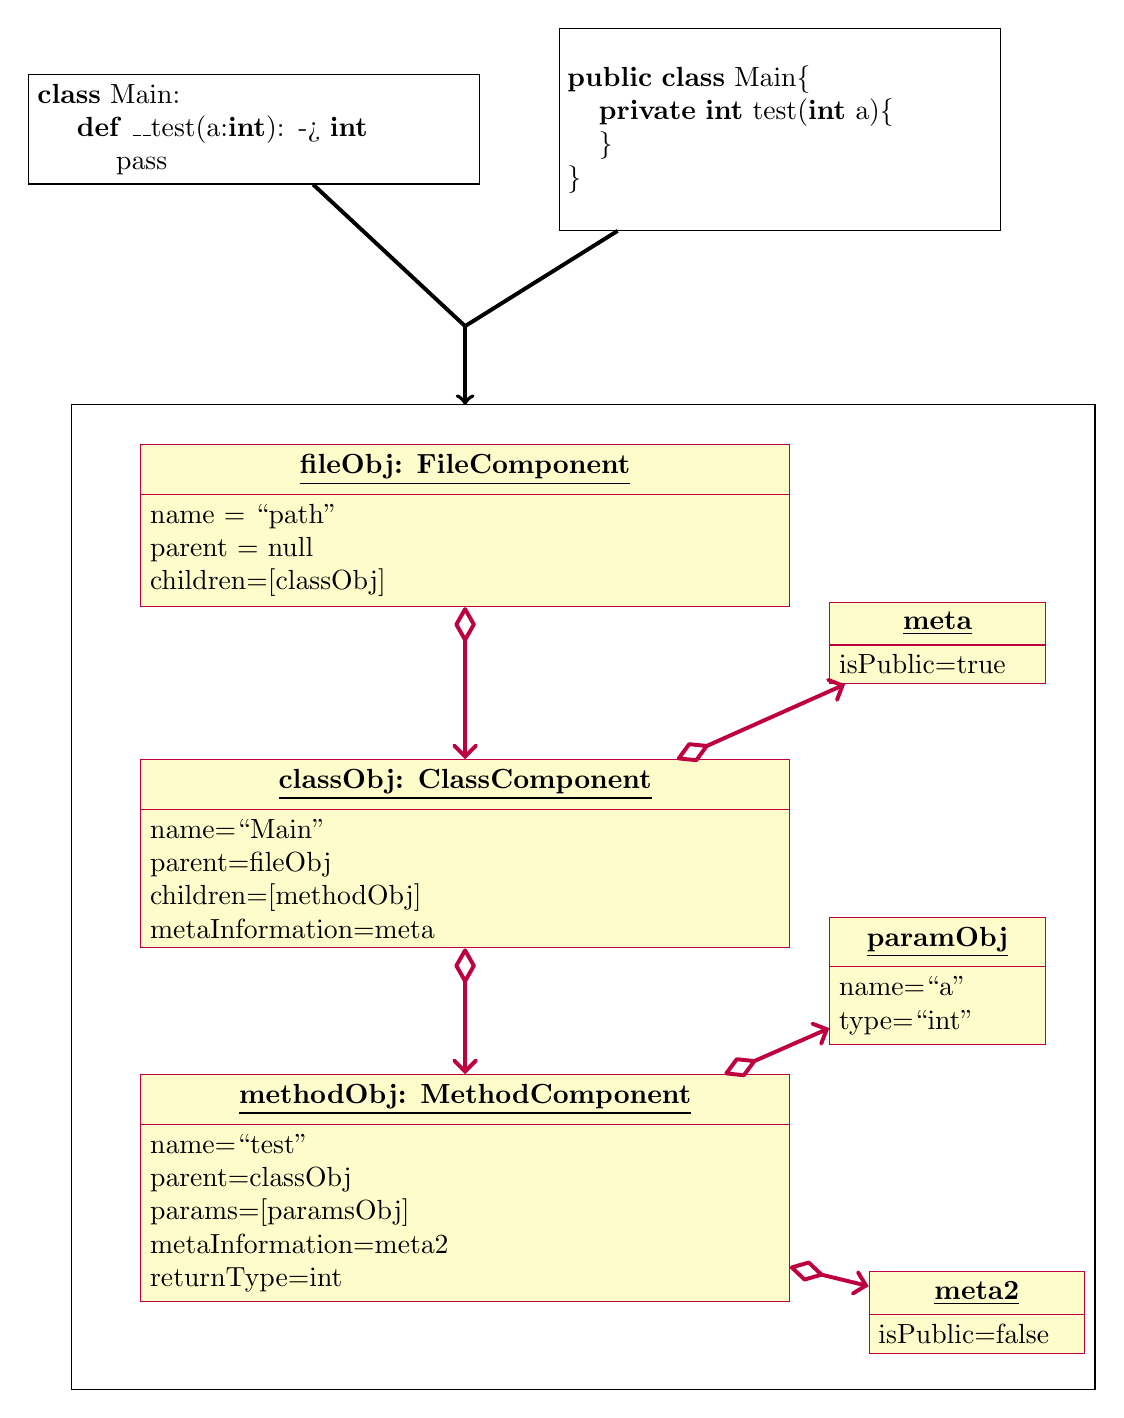
\begin{tikzpicture}
 \pgfmathsetlengthmacro\breite{6cm}
\pgfmathsetlengthmacro\hoehe{2.567cm}
\pgfmathsetlengthmacro\InnerSep{0.4cm}
\node[draw,
anchor=center, 
inner sep=0pt, 
minimum width=5cm, text width=6cm-\InnerSep,
align=justify,
minimum height=\hoehe
] (java) {
  \hspace*{0.1cm}\textbf{public} \textbf{class} Main\{\newline 
     \hspace*{0.5cm}\textbf{private} \textbf{int} test(\textbf{int} a)\{\newline
    \hspace*{0.5cm}\}\newline
\hspace*{0.1cm}\}

};
\node[draw,text width=5.5cm, left = of java](python){
\textbf{class} Main:\newline
     \hspace*{0.5cm}\textbf{def} \_\_test(a:\textbf{int}): -> \textbf{int}\newline
         \hspace*{1cm}pass

};
\draw[line width=0.05cm] (python) -- (-4,-2.5) ;
\draw [line width=0.05cm](java) -- (-4,-2.5);
\draw[->,thick,line width=0.05cm] (-4,-2.5) -- (-4,-3.5);
\draw [] (-9,-3.5) rectangle(4,-16);
\begin{scope} {0,-10}
       \begin{object}[text width=8cm]{fileObj}{-4,-4}
        \instanceOf{FileComponent}
        \attribute{name = \enquote{path}}
        \attribute{parent = null}
        \attribute{children={[}classObj{]}}
      \end{object}
      \begin{object}[text width=8cm]{classObj}{-4,-8 }
        \instanceOf{ClassComponent}
        \attribute{name=\enquote{Main}}
        \attribute{parent=fileObj}
        \attribute{children={[}methodObj{]}}
          \attribute{metaInformation=meta}
      \end{object}
    \begin{object}[text width=8cm]{methodObj}{-4,-12}
        \instanceOf{MethodComponent}
        \attribute{name=\enquote{test}}
        \attribute{parent=classObj}
        \attribute{params={[}paramsObj{]}}
        \attribute{metaInformation=meta2}
        \attribute{returnType=int}
      \end{object}
      \begin{object}[text width=2.5cm]{paramObj}{2,-10}
        \attribute{name=\enquote{a}}
        \attribute{type=\enquote{int}}
      \end{object}
    \begin{object}[text width=2.5cm]{meta}{2,-6}
        \attribute{isPublic=true}
      \end{object}
    \begin{object}[text width=2.5cm]{meta2}{2.5,-14.5}
        \attribute{isPublic=false}
      \end{object}
\end{scope}
\begin{scope}[line width=0.05cm]
    \aggregation{fileObj}{}{}{classObj}{}{}
     \aggregation {classObj}{}{}{methodObj}{}{}
      \aggregation {methodObj}{}{}{paramObj}{}{}
    \aggregation {classObj}{}{}{meta}{}{}
        \aggregation {methodObj}{}{}{meta2}{}{}
\end{scope}

    
\end{tikzpicture}
}
     
     \caption{Objektdiagramm aus Java- und Python-Code}
     \label{fig:python_java_comp}
 \end{figure}

Abbildung \ref{fig:python_java_comp} veranschaulicht, wie eine einfache Datei in die Objektstruktur umgewandelt werden kann. Dabei werden eine einfache Java-Datei und eine semantisch äquivalente Python-Datei als Beispiel verwendet, um zu zeigen, dass aus beiden Sprachen eine gleiche Objektstruktur erzeugt werden kann. Dabei wurden zur Übersichtlichkeit einige nicht relevanten Attribute entfernt.



Das Programm in beiden Sprachen besteht aus einer öffentlichen Klasse \textit{Main} und einer privaten Methode \textit{test}, die einen Parameter \textit{a} als Ganzzahl erhält und eine Ganzzahl zurückgibt. Die höchste Hierarchieebene ist immer ein \textit{FileComponent}. Diese Datei enthält hier genau ein Kind namens \textit{classObj}, könnte aber in anderen Fällen auch mehrere Kinder (wie z.~B. Klassen enthalten). Die Klasse besitzt zudem einen Verweis auf ihren Elternteil. Außerdem enthält das \textit{classObj} eine Referenz auf Metainformationen, die hier nur angeben, dass die Klasse öffentlich ist. In diesen Metainformationen könnten auch andere relativ sprachspezifische Informationen definiert werden, falls sie für Metriken relevant sein könnten. Die Klasse enthält wiederum genau die Methode als einziges Kind. Die Methode hat ebenfalls einen Verweis auf die Metainformationen, welche die Methode als privat markieren. Außerdem hat die Methode einen \textit{returnType} und einen Verweis auf die Liste der Parameter, die wiederum aus einem Namen und einem Datentyp bestehen. Das Feld \textit{comment}, welches einen Verweis auf den strukturierten Kommentar liefert, wird in dieser Abbildung nicht dargestellt, da es bei den Dateien keine Dokumentation gibt und es somit den Wert \textit{null} hat.

Die Beziehungen der Klassen, die für das Parsing zuständig sind, werden zusätzlich in Abbildung \ref{fig:uml_parsing} im Anhang \ref{appendix_parsing_uml}. als UML-Diagramm illustriert.

\subsubsection{Repräsentation der strukturierten Kommentare}\label{chapter:structured_comments}
Neben der hierarchischen Repräsentation der einzelnen Komponenten müssen auch die strukturierten Kommentare (wie z.~B. Javadoc) geeignet in eine Datenstruktur umgewandelt werden. Wie in Kapitel \ref{chapter:javadoc}
 erläutert, besteht ein strukturierter Kommentar in vielen Fällen aus zwei Teilen. Der erste Teil ist eine allgemeine Beschreibung der Komponente. Im zweiten Teil werden bestimmte Strukturen genauer erläutert. So können einzelne Parameter erklärt werden oder der Rückgabewert beschrieben werden. 
 Dieser Aufbau findet sich auch in \textit{Doxygen} \cite{doxygen} oder \textit{Docstring} \cite{docstring}, sodass diese Struktur als Grundlage genommen wird. 
 
 Ein strukturierter Kommentar besteht also aus einer generellen Beschreibung, die auch weggelassen werden kann. Anschließend folgen null bis beliebig viele Tags. Jeder Tag besteht aus einem Typ (z.~B. \enquote{@param}, \enquote{@return} oder \enquote{@throws}), einem optionalen Parameter, welcher von einigen Tags benötigt wird und der Beschreibung des Tags. Die Namen der Tags sind generalisiert, dies bedeutet, dass unabhängig von der Programmiersprache der Tag zur Beschreibung eines Parameters immer \enquote{@param} heißen muss. Dies muss bei der Entwicklung eines Parsers beachtet werden. 
 
 Ein strukturierter Kommentar kann ebenfalls spezielle Elemente (wie z.~B. \ac{HTML}-Elemente oder Inline-Tags) enthalten. Hier werden diese Elemente unverarbeitet gelassen, also unverändert mit dem Rest des Kommentars als Zeichenkette gespeichert. Metriken, die diese Informationen benötigen, müssen diese Elemente also selbstständig extrahieren. Andere Metriken (wie z.~B. die Metriken in Kapitel \ref{chapter:metrics_semantic}) benötigen diese speziellen Elemente nicht, sodass eine einheitliche Schnittstelle, die sowohl die natürliche Sprache als auch die speziellen Elemente berücksichtigt und  zudem relativ programmiersprachenunabhängig sein müsste, viele Herausforderungen mit sich bringt.   
 
 Wird kein strukturierter Kommentar angegeben, so liefert der entsprechende Getter \textit{getComment} den Wert \enquote{null} zurück. 
\section{Konzeption der Metriken}\label{chapter:metric_conception}
Nachdem eine Datei in ihre einzelnen Komponenten zerlegt wurde, kann die Qualität der Softwaredokumentation überprüft werden. Jede gefundene Komponente besitzt einen Verweis auf die dazugehörige Dokumentation, die bei Nichtvorhandensein auch null sein kann. Anhand dieser Referenz kann geprüft werden, ob die Softwaredokumentation der Komponente ausreichend ist. Zur Bewertung der Dokumentation gibt es verschiedene  Möglichkeiten. Beispielsweise könnte überprüft werden, ob eine Komponente dokumentiert oder undokumentiert ist. Eine weitere Möglichkeit wäre es, die Verständlichkeit der Dokumentation zu prüfen. Alle diese Vorgehensweisen basieren auf Metriken, die auf wissenschaftliche Studien beruhen oder zumindest plausibel sind. In diesem Abschnitt wird ein Konzept erläutert, um eine Metrik zu implementieren. Anschließend wird beschrieben, wie die Ergebnisse jeder Metrik zusammengefasst werden, um ein Endresultat zu erhalten. 

\subsection{Implementation einer Metrik}\label{chapter:metric_impl}
Damit eine Metrik die Dokumentation bewerten kann, benötigt sie Zugriff auf die Komponente. Außerdem muss sie ihr Ergebnis irgendwie veröffentlichen bzw. zwischenspeichern, damit es später weiterverarbeitet werden kann. Des Weiteren ist nicht jede Metrik mit jeder Komponente kompatibel. Eine Metrik, die überprüft, ob jeder Methodenparameter dokumentiert ist, kann diese Aufgabe bei anderen Komponentenarten nicht erfüllen. Zudem sollte es die Möglichkeit geben, das Verhalten einer Metrik mittels Parameter anzupassen, damit die Metrik konfigurierbar bleibt. Außerdem sollte eine Metrik bei der Bewertung auch begründen, warum die Dokumentation einer Komponente nicht ausreichend ist. Zuletzt soll der Benutzer des Tools selbst auswählen können, welche Metriken angewendet werden sollen, da nicht jede Metrik immer sinnvoll ist. 

Eine Möglichkeit, diese Anforderung für eine Metrik umzusetzen, ist die Verwendung einer Methode pro Metrik, welche die Komponente und die Parameter als Eingabe erhält und daraus die Bewertung und eventuelle Begründung ermittelt und zurückgibt. Allerdings ist dieser Ansatz sehr prozedural, denn es gibt beispielsweise keine Kapselung zwischen den Metriken.  

Ein anderer Ansatz, der hier auch gewählt wird, ist es, jede gewünschte Metrik als Klasse zu implementieren. Jede implementierte Metrik kann somit die notwendigen Berechnungen abgekapselt von anderen Metriken erledigen, was die Wartbarkeit verbessert. Um trotzdem für eine einheitliche Schnittstelle zu sorgen, muss jede zu implementierende Metrik von einer abstrakten Basisklasse \textit{(DocumentationAnalysisMetric)} erben. Wenn eine neue Metrik implementiert werden soll, muss eine neue Klasse erstellt werden, die von dieser abstrakten Basisklasse erbt. Eine Instanz dieser Klasse wird im Folgenden \textbf{Metrikobjekt} genannt und repräsentiert eine konkrete Implementierung der Metrik, die bei der Bewertung der Dokumentation berücksichtigt werden kann. Um diese Bewertung durchzuführen, muss geprüft werden, ob eine Metrik mit einer Komponente kompatibel ist. Dies wird durch die  Methode \textit{shallConsider} erledigt,  welche dementsprechend einen Wahrheitswert zurückgibt. Die anschließende Analyse erfolgt durch die Methode \textit{analyze}. Diese führt den metrikspezifischen Algorithmus aus und speichert das Ergebnis wie in Kapitel \ref{chapter:store_metric} beschrieben, damit es zu einem Gesamtergebnis verarbeitet werden kann.

Da eine Metrik auch parametrisierbar sein soll, müssen bei der Instanziierung  eines Metrikobjektes Parameter übergeben werden, die von der Implementation der Metrik zur Modifikation des Verhaltens der Metrik verwendet werden können. Diese Parameter werden sehr abhängig von der Metrik sein, sodass eine einheitliche Schnittstelle nur schwer umsetzbar ist. Daher werden die Parameter als Datentyp \textit{any} übergeben, sodass es keine Typüberprüfung gibt. Alternativ wäre eine assoziative Liste möglich, bei dem ein Parametername als Zeichenkette ein Wert zugeordnet wird, aber auch hier könnte keine Überprüfung eines Datentypes vorgenommen werden. 

Eine  weitere Voraussetzung für ein Metrikobjekt ist ein eindeutiger Name. Dadurch kann die gleiche Metrik mit unterschiedlichen Parametern verwendet werden. Außerdem wird so eine Zuordnung von Gewichten vereinfacht. Standardmäßig besteht dieser eindeutige Name aus dem Namen der implementierten Metrik, gefolgt von einem Unterstrich und einer fortlaufenden Nummer. 

Ein UML-Diagramm der relevanten Klassen, die für die Berechnung der Dokumentationsqualität zuständig sind, befindet sich in Abbildung \ref{fig:uml_metrics} im Anhang \ref{appendix_metrics_uml}.


\subsubsection{Bewertung der Dokumentation}
Die Methode \textit{analyze} muss eine Bewertung darüber abgeben, ob die Qualität der Dokumentation ausreichend ist. Für die Repräsentation dieser Bewertung gibt es viele Möglichkeiten, allerdings ist eine numerische Bewertung mittels einer Intervallskala am sinnvollsten, da so der arithmetische Mittelwert, der Median etc. berechnet werden kann, was für die Bildung des Gesamtergebnisses wichtig ist.
Die numerische Bewertung soll eine Aussage über die Dokumentationsqualität liefern. Eine Bewertung von 0 steht für eine sehr schlechte bis nicht existente Dokumentation und die Bewertung 100 steht für eine exzellente Dokumentation, sodass die Bewertung sich als Prozent lesen lassen kann. Das Ergebnis einer implementierten Metrik sollte diesen Wertebereich nicht verlassen, da eine Fehlerbehandlung nicht implementiert ist. Bei Metriken, die per Design schon einen prozentualen Wert zurückgeben, wird diese Vorgabe stets eingehalten. Bei anderen Metriken (z.~B. die Flesch-Metrik in Kapitel \ref{chapter:metrics_semantic}) sollte eine mathematische Funktion gefunden werden, die das Ergebnis der Metrik auf den Wertebereich 0 bis 100 abbildet. Die genaue Umsetzung hängt von der Metrik ab. In jedem Falle sollte es für eine Metrik Ergebnisse geben, die auf eine gute bzw. schlechte Dokumentation hindeuten, damit diese auf 100 bzw. 0 abgebildet werden können. Nur durch diese Einschränkung auf einen fixen Wertebereich ist es möglich, den Mittelwert, Median etc. zu bilden und so eine Vergleichbarkeit zu ermöglichen. 

\subsubsection{Verwaltung der Metriken}

Für die spätere Ausführung der Metriken ist es sinnvoll, eine zentrale Stelle zu haben, welche die Verwaltung der Metriken übernimmt. Diese zentrale Stelle entkoppelt die Verwaltung der Metriken von dem restlichen Programmcode und sorgt so für eine bessere Struktur des Programms. Diese zentrale Komponente ist der \textbf{Metrikmanager}. Der Metrikmanager ist eine statische Klasse, die von allen Modulen des Tools benutzt werden kann, welche mit den Metriken arbeiten müssen.  

Eine wichtige Funktion des Metrikmanagers ist das Erzeugen neuer Metriken. Zwar wäre es möglich, die Metriken direkt zu instanziieren, wenn sie benötigt werden, allerdings entsteht dadurch eine direkte Abhängigkeit zwischen der Metrik und dem Modul, welches eine Metrik erzeugen möchte. Zur Vermeidung dieser direkten Abhängigkeit können Fabrikmethoden verwendet werden, bei dem ein Objekt nicht direkt erzeugt wird, sondern mittels einer Abfrage durch eine bestimmte Methode erzeugt wird und anschließend an das anfragende Objekt zurückgegeben wird \cite[S.~149--161]{gamma2015design}.

Basierend auf dieser Idee kann ein Modul, das ein konkretes Metrikobjekt benötigt, den Metrikmanager mit der Instanziierung beauftragen. Dabei benötigt der Metrikmanager eine Zeichenkette, um eine konkrete abgeleitete Klasse zu identifizieren, von der das neue Metrikobjekt instanziiert werden soll. Diese Zeichenkette wird eindeutig einer bestimmten abgeleiteten Klasse zugeordnet, sodass bei der Implementation einer neuen Metrik ein neuer Name spezifiziert werden muss. Alle Zeichenketten, die für eine bestimmte Metrik stehen, werden in einer Konstantensammlung  (\textit{Enum}) definiert, die ebenfalls bei der Definition einer neuen Metrik ergänzt werden muss.  Das neue Metrikobjekt benötigt, wie in Kapitel \ref{chapter:metric_impl} beschrieben, zudem einen eindeutigen Namen und Parameter, damit es eindeutig auffindbar ist und korrekt arbeiten kann. Dieses neue Metrikobjekt wird zudem vom Metrikmanager registriert und in einer Liste gespeichert, damit es später möglich sein wird, über alle erzeugten Metriken zu iterieren. 

Der Metrikmanager bietet zudem eine Methode an, mit denen der Standardwerte für die Parameter einer Metrik abgerufen werden können, sodass diese an einer Stelle verwaltet werden können. Außerdem kann der Metrikmanager auch einen \textit{MetricResultBuilder} erzeugen, um Teilergebnisse zu einem Gesamtresultat zu aggregieren. Dies geschieht ebenfalls über eine Fabrikmethode, sodass auch hier eine Entkopplung stattfindet. 

\subsubsection{Sprachspezifische Informationen für Metriken}\label{chapter:langSpec}
Da das Tool für möglichst viele objektorientierte Programmiersprachen konzipiert werden soll, muss eine Generalisierung erfolgen, da jede Sprache ihre Eigenheiten hat und möglicherweise besondere Funktionen anbietet, die nur schwer in einem abstrakten Format zu bringen sind.

Nichtsdestotrotz können solche sprachspezifischen Eigenheiten auch in der Dokumentation erwähnt werden. Daher ist es eine sinnvolle Idee, dass Metriken auch diese Besonderheiten benutzen, um ein genaueres Bild der Dokumentationsqualität zu erfahren, ohne jedoch zu wissen, welche Programmiersprache gerade analysiert wird. Beispielsweise können die Checked-Ausnahmen in Java mit den Informationen in der Javadoc verglichen werden. Auch können hierdurch überschriebene Methoden ignoriert werden, da diese oft nicht mehr dokumentiert werden müssen.

Um solche sprachspezifischen Analysen zu erlauben, besitzt jede Metrik Zugriff auf ein Objekt der Klasse \textit{LanguageSpecificHelper}. Wenn eine neue Programmiersprache hinzugefügt werden soll, kann von dieser geerbt werden. In der Klasse \textit{LanguageSpecificHelper} sind bereits einige Methoden definiert, die einigen Metriken bei der Bewertung helfen. So bewertet die Methode \textit{rateDocumentationCompatibility}, ob die Dokumentation alle sprachspezifischen Informationen erläutert (z.~B. \enquote{@throws}). Die Methode \textit{shallConsider} kann genutzt werden, um überschriebene Methoden zu ignorieren. 

Um eine eigene Methoden hinzuzufügen, muss diese in der Basisklasse definiert werden. Diese Methode sollte in der Basisklasse keine Aktionen durchführen, sondern entweder gar nichts tun oder Rückgabewerte haben, die keinen Einfluss auf Metriken haben. Anschließend kann diese Methode in einer sprachspezifischen abgeleiteten Klasse der Basisklasse korrekt implementiert werden. Die entsprechende Methode kann dann durch Änderung des Quellcodes der Metrik an den passenden Stellen von der Metrik verwendet werden. So kann beispielsweise das Resultat einer Metrik modifiziert werden oder weitere Ergebnisse mittels des \textit{MetricResultBuilders} angefügt werden.

\subsection{Einzelergebnisse verarbeiten}\label{chapter:store_metric}

Das berechnete Ergebnis einer Komponente muss nun gespeichert werden, damit es später ausgewertet werden kann. Dazu wird ein \textit{MetricResult}-Objekt erstellt, welches das im vorherigen Unterabschnitt berechnete Ergebnis enthält. Außerdem werden hier eventuelle Begründungen und Hinweise gespeichert, die den Anwender dabei unterstützen, die Qualität der Dokumentation zu verbessern. Jede Begründung enthält den Dateipfad der betroffenen Datei, den Namen der bemängelten Komponente und ein Zeilennummerintervall, sodass der Benutzer die problematische Stelle schnell finden kann. Zuletzt werden noch Informationen gespeichert, die beschreiben, in welchem Kontext das Ergebnis produziert wurde. Dies ist für die Gewichtung der Einzelergebnisse notwendig und wird in den nächsten Unterabschnitten noch genauer erläutert. 

Für die Speicherung des Objektes gibt es zwei Möglichkeiten. Die erste Möglichkeit wäre es, dass die \textit{analyze}-Methode das \textit{MetricResult}-Objekt zurückgibt, sodass der Aufrufer damit arbeiten kann. Bei der zweiten Möglichkeit wird das Ergebnis einem anderen Objekt übergeben, der dann die Weiterverarbeitung vornimmt. Dies hat den Vorteil, dass eine Metrik kein Ergebnis zurückliefern muss, wenn es kein sinnvolles Ergebnis berechnen kann. Bei einem Rückgabewert müsste ansonsten ein ungültiger Wert wie z.~B. \textit{null} vereinbart werden. Außerdem kann eine Metrik auch mehrere Resultate speichern, was bei komplexeren Komponenten in Betracht gezogen werden könnte. Dieses weitere Objekt ist ein  \textit{MetricResultBuilder}, der wie im nächsten Unterabschnitt beschrieben, die Softwaredokumentationsqualität jeder Komponente sammelt und daraus ein Gesamtergebnis berechnet.  

\subsubsection{Einzelergebnisse aggregieren}
Da ein Softwareprojekt aus Tausenden von Dateien bestehen kann, die wiederum aus verschiedenen Komponenten bestehen, müssen die Einzelergebnisse aggregiert werden, um so am Ende ein Gesamtergebnis zu erhalten, das zur Einschätzung der Qualität der Softwaredokumentation genutzt werden kann. Dazu wird dem \textit{MetricResultBuilder} jedes Ergebnis mittels der \textit{processResult}-Methode mitgeteilt, welches das Ergebnis in einer Liste speichert. Wenn alle Metriken verarbeitet sind, wird daraus ein Gesamtresultat gebildet. Dies geschieht durch die Methode \textit{getAggregratedResult}. Dabei wird standardmäßig ein arithmetischer Mittelwert gebildet.

Neue Algorithmen (wie z.~B. der Median oder der gewichtete Mittelwert) können implementiert werden, indem von dieser Klasse abgeleitet wird und die \textit{getAggregratedResult}-Methode überschrieben wird. 

Ein \textit{ResultBuilder} basiert auf dem Vorbild des Design-Patterns \enquote{Builder} aus \cite[S. 139--149]{gamma2015design}, da dieser aus einzelnen Metrikresultaten ein vollständiges Metrikergebnis baut.


 
\subsubsection{Zuordnung der Gewichte}\label{chapter_weights_assign}
Für einige Algorithmen muss eine Gewichtung vorgenommen werden, um bestimmte Ergebnisse besser oder schlechter zu bewerten. Dazu muss jedes Teilergebnis ein Gewicht zugeordnet werden. 

Insgesamt kann ein Teilergebnis anhand von drei Kategorien gewichtet werden. Durch die Gewichtung aufgrund der verwendeten Metrik können bestimmten Metriken einen größeren Einfluss auf das Gesamtergebnis haben, wenn diese als vertrauenswürdiger empfunden werden. Durch die Gewichtung von Dateien kann beispielsweise die öffentliche Schnittstelle einen größeren Einfluss auf die Bewertung nehmen, da diese Komponenten bzw. Dateien sehr kritisch sein können und daher gut verstanden werden müssen. Auch eine Gewichtung nach Komponenten kann in bestimmten Situationen sinnvoll sein. So kann beispielsweise argumentiert werden, dass Methoden, die durch ihre Parameter, Rückgabewerte und geworfenen Ausnahmen komplexer als Felder sind, höher gewichtet werden sollen.

Die Zuordnung der Gewichte erfolgt über einen \textit{WeightResolver}, welches eine Schnittstelle anbietet, um einen Bezeichner auf ein Gewicht abzubilden. Bei dem eindeutigen Namen eines Metrikobjektes kann hierfür eine assoziative Liste verwendet werden. Auch bei Komponenten, die durch ihren Klassennamen (wie z.~B. \textit{ClassComponent}) repräsentiert werden, ist  eine solche assoziative Liste sinnvoll, da nur eine begrenzte Anzahl an Metriken bzw. Komponenten existieren kann.
Für Dateipfade ist dies allerdings nicht praktikabel, da es eine Vielzahl an Dateien geben kann. Stattdessen können hier ähnlich wie bei der Filterung von Dateien in Kapitel \ref{chapter:traversing} Wildcard-Patterns verwendet werden. Eine assoziative Liste kann dazu jedes Wildcard-Patterns und das dazugehörige Gewicht speichern. Bei einer Abfrage kann das Gewicht des ersten Eintrages zurückgegeben werden, bei dem der Dateipfad mit dem Wildcard-Pattern kompatibel ist. Dies ermöglicht es, ganze Verzeichnisse oder Dateien mit bestimmten Namen stärker zu gewichten. 

Bei der Suche nach dem passenden Gewicht zu den Dateien und Komponenten kann es vorkommen, dass das passende Gewicht nicht gefunden wird. Um hierdurch entstehende Probleme zu vermeiden, wird ein Standardwert genommen (z.~B. 1). 

Jedes \textit{MetricResult}-Objekt enthält ein Tupel von drei Namen, welche die Quelle dieses Ergebnisses repräsentieren (Dateipfad, Komponententyp und eindeutiger Metrikname). Der Dateipfad beschreibt, in welcher Datei die Komponente liegt, die durch dieses Teilergebnis analysiert wurde. Der Komponententyp enthält den Klassennamen der Komponente und gibt somit Aufschluss darüber, ob diese Komponente eine Klasse, Methode etc. ist. Bei einer Klasse würde beispielsweise die Zeichenkette \enquote{ClassComponent} gespeichert werden. Durch den eindeutigen Metrikname (siehe Kapitel \ref{chapter:metric_impl}) wird  festgelegt, welche Metrik dieses Teilresultat produzierte. Alternativ könnte auch hier der Klassenname der Metrik verwendet werden. Allerdings kann eine Metrik durch Verwendung verschiedener Parameter auch mehrfach angewendet werden, sodass eine unterschiedliche Gewichtung möglich wäre. Daher ist der eindeutige Name hier sinnvoller.

  \begin{figure}[h!]
  \centering
 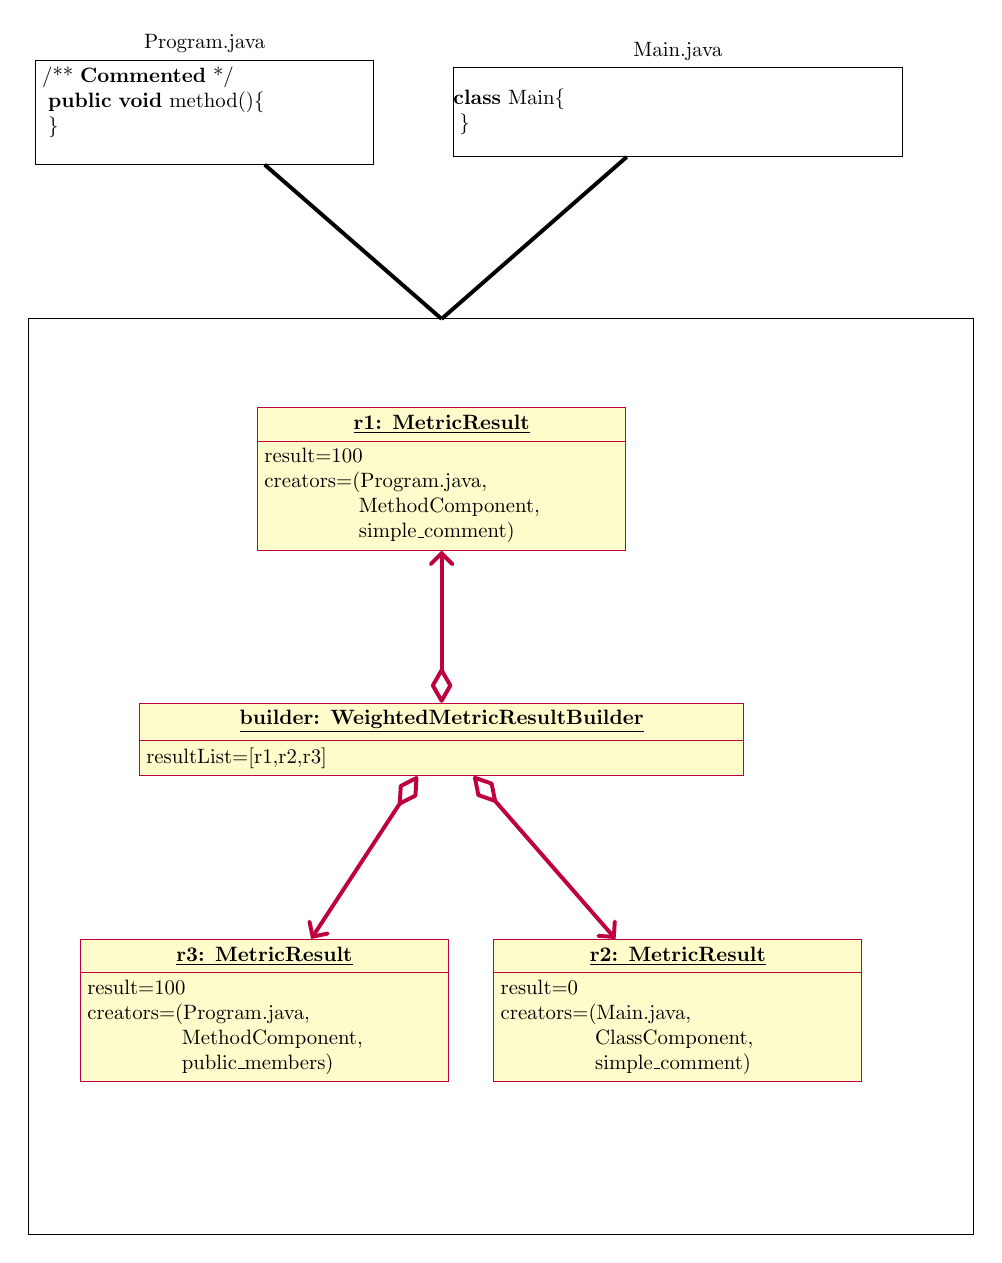
\begin{tikzpicture}[scale=0.75, every node/.style={scale=0.75}]
 \pgfmathsetlengthmacro\breite{6cm}
\pgfmathsetlengthmacro\hoehe{2.567cm}
\pgfmathsetlengthmacro\InnerSep{0.4cm}
\node[draw,
anchor=center, 
inner sep=0pt, 
minimum width=5cm, text width=8cm-\InnerSep,
align=justify,minimum height=1.5cm] (java) {\textbf{class} Main\{\newline 
\hspace*{0.1cm}\}};

\node[draw,text width=5.5cm, left = of java](java2){
/** \textbf{Commented} */ \newline
     \hspace*{0.1cm}\textbf{public} \textbf{void} method()\{\newline
    \hspace*{0.1cm}\}\newline
};
\draw[line width=0.05cm]    (java2) -- (-4,-3.5) ;
\draw [line width=0.05cm](java) -- (-4,-3.5);
\draw[thick,line width=0.05cm] (-4,-3.5) -- (-4,-3.5);

\node[above=-0.0 of java2,line width=0cm]{Program.java};

\node[above=-0.0 of java,line width=0cm]{Main.java};


\draw [] (-11,-3.5) rectangle(5,-19);
\begin{scope} {0,-10}
       \begin{object}[text width=10cm]{builder}{-4,-10}
        \instanceOf{WeightedMetricResultBuilder}
        \attribute{resultList={[r1,r2,r3]}}
      \end{object}
      \begin{object}[text width=6cm]{r1}{-4,-5 }
        \instanceOf{MetricResult}
        \attribute{result=100}
        \attribute{creators=(Program.java,\newline
        \hspace*{1.6cm}MethodComponent, \newline
        \hspace*{1.6cm}simple\_comment)}
      \end{object}
      
        \begin{object}[text width=6cm]{r2}{0,-14 }
        \instanceOf{MetricResult}
        \attribute{result=0}
        \attribute{creators=(Main.java,\newline
        \hspace*{1.6cm}ClassComponent,\newline
        \hspace*{1.6cm}simple\_comment)}
      \end{object}
      
           \begin{object}[text width=6cm]{r3}{-7,-14 }
        \instanceOf{MetricResult}
        \attribute{result=100}
        \attribute{creators=(Program.java,\newline
       \hspace*{1.6cm}MethodComponent,\newline
       \hspace*{1.6cm}public\_members)}
      \end{object}
      

   
\end{scope}
\begin{scope}[line width=0.05cm]
    \aggregation{builder}{}{}{r1}{}{}
    \aggregation{builder}{}{}{r2}{}{}
    \aggregation{builder}{}{}{r3}{}{}

\end{scope}

    
\end{tikzpicture}
     
     \caption{ Veranschaulichung der Bildung eines Gesamtergebnisses}
     \label{fig:metric_weighting}
 \end{figure}
Durch dieses Tupel kann für jedes Teilergebnis die Gewichtung der Metrik, der Komponente und des Dateipfades  abgerufen werden. Durch Multiplikation  aller Gewichtungen entsteht ein Gesamtgewicht.

Abbildung \ref{fig:metric_weighting} veranschaulicht anhand eines vereinfachten Objektdiagramms die Bildung eines Gesamtresultats mittels Gewichtung von verschiedenen Ergebnissen, indem der gewichtete Mittelwert aus Kapitel \ref{chapter:weighted_aggreg} verwendet wird. Hier wird ein hypothetisches Projekt mit zwei Dateien analysiert. Die erste Datei \enquote{Program.java} enthält nur eine öffentliche Methode \textit{method}, was in Java eigentlich nicht möglich ist, aber hier zur Vereinfachung zugelassen sein soll. Die zweite Datei \enquote{Main.java} enthält eine nichtöffentliche Klasse \textit{Main}. In diesem Beispiel werden zwei Metriken verwendet. Die erste Metrik prüft das Vorhandensein der Dokumentation bei allen Komponenten, während die zweite Metrik nur öffentliche Komponenten betrachtet (siehe Kapitel \ref{chapter:metrics_coverage}). In diesem Beispiel soll die Datei \enquote{Main.java} mit dem Faktor $3$ gewichtet werden. Methoden sollen mit dem Faktor $4$ gewichtet werden. Die zweite Metrik \textit{public\_members} wird mit dem Faktor $2$ gewichtet. Alle anderen Dateien, Komponenten und Metriken werden mit dem Standardfaktor $1$ gewichtet.

Das erste Teilergebnis \textit{r1} ist 100, da es die  Methode \textit{method} beschreibt, welche dokumentiert ist. Auch das dritte Teilergebnis \textit{r3} hat den Wert 100, da es die gleiche Komponente nur mit der zweiten Metrik beschreibt. Das zweite Teilergebnis \textit{r2} hat den Wert 0, da es die undokumentierte Klasse \textit{Main} beschreibt.  Es gibt kein weiteres Teilergebnis von \enquote{Main.java}, da die zweite Metrik jegliche nichtöffentliche Komponenten ignoriert. Die Teilergebnisse werden durch den \textit{WeightedMetricResultBuilder} intern gespeichert. 

Das Teilergebnis jeder gefundenen Komponente enthält gemäß dem obigen Vorgehen ein Tupel aus Dateiname, Komponentenname und Metrikname. Beispielsweise enthält das erste  Teilergebnis \textit{r1} das Tupel \enquote{(Program.java, MethodComponent, simple\_comment)}, wobei die einzelnen Bestandteile des Tupels Zeichenketten sind. Basierend auf diesen Informationen kann der \textit{WeightedResultBuilder} eine Gewichtung vornehmen. Das erste Teilergebnis würde mit dem Faktor $1*4*1=4$ gewichtet werden, da es von einer Methode stammt  und ansonsten nicht besonders gewichtet wird. Das zweite Teilergebnis erhält das Gewicht $3*1*1=3$, da es von der Datei \enquote{Main.java} stammt. Zuletzt besitzt das dritte Teilresultat die Gewichtung $1*4*2=2$, da es von der zweiten Metrik berechnet wurde und auch von einer Methode stammt. 

Basierend auf diesen Teilresultaten kann ein Gesamtergebnis berechnet werden. Hierzu wird jedes Ergebnis mit dessen Gewicht multipliziert und anschließend wird durch die Summe der Gewichte geteilt. Bezogen auf das Beispiel würde die Rechnung folgendermaßen aussehen:
\begin{equation}
    \frac{4*100 + 3*0 + 8*100}{4+3+8}=80
\end{equation}
Dieses Ergebnis ist dann Maß für die Bewertung der Dokumentationsqualität dieses hypothetischen Projektes. 










\begingroup
\renewcommand{\cleardoublepage}{} % TODO maybe removing this and next
\renewcommand{\clearpage}{}
\chapter{Umsetzung}\label{chapter:program}
\endgroup
In diesem Kapitel wird auf die Umsetzung der in Kapitel \ref{chapter_conception} beschriebenen Architektur eingegangen. In Kapitel \ref{chapter:tool_running} wird zunächst erläutert, wie das Programm konkret ausgeführt wird, um die Dokumentationsqualität zu ermitteln. Danach wird in Kapitel \ref{chapter:traversing} beschrieben, wie das Programm die einzelnen Java-Dateien findet, damit diese weiterverarbeitet werden können.  Außerdem wird in Kapitel \ref{chapter:antlr4_impl} erläutert, wie ANTLR4 verwendet wird, um Java-Dateien zu parsen. Daraufhin wird erklärt, wie die strukturierten Kommentare geparst werden (Kapitel \ref{chapter:comment_parsing}).  In Kapitel \ref{chapter:conf} wird die Konfiguration des Tools erläutert. Um auch einen Vergleich zwischen den aktuellen und den vorherigen Zustand der Dokumentationsqualität zu ermöglichen, wird in Kapitel \ref{chapter:saving} beschrieben, wie das letzte Ergebnis der Bewertung gespeichert werden kann. In Kapitel \ref{chapter:github_actions_impl} wird erklärt, wie das Programm in GitHub Actions eingebunden wird und wie es so genutzt werden kann. Zum Abschluss werden in Kapitel \ref{chapter:metrics} und \ref{chapter:algos_aggregation} die implementierten Metriken und die implementierten Aggregationsalgorithmen erläutert. 


\hfill
\section{Ausführung des Programms}\label{chapter:tool_running}
In diesem Unterabschnitt wird beschrieben, wie das Programm die in Kapitel \ref{chapter_conception}
beschriebenen Arbeitspakete nutzt, um die Qualität der Softwaredokumentation zu bewerten. 

Die Koordination des Programms wird in der Datei \enquote{index.ts} durchgeführt, die als Einstiegspunkt des Programms verstanden werden kann. In dieser Datei werden die einzelnen Module des Programms in der richtigen Reihenfolge aufgerufen und die Ergebnisse eines Moduls werden durch die \enquote{index.ts}-Datei an das folgende Modul/Arbeitspaket übergeben, soweit sie dort benötigt werden. Dadurch sind die Module voneinander entkoppelt und greifen nicht direkt aufeinander zu. 

Im ersten Schritt  muss die Konfiguration des Programms geladen werden. Dazu wird das Arbeitsverzeichnis von der Kommandozeile gelesen. Basierend auf das Arbeitsverzeichnis kann dann die Konfiguration des Tools geladen werden, wie es in Kapitel \ref{chapter:conf} beschrieben ist.  

Anschließend müssen einige Objekte  initialisiert werden. Hierzu werden die Werte aus der Konfiguration (z.~B. der Konfigurationsdatei) verwendet. Beispielsweise kann durch \textit{builder} der Algorithmus festgelegt werden, der die Einzelergebnisse der einzelnen Metriken zu einem Gesamtresultat kombiniert. Dazu wird eine Fabrikmethode verwendet, da damit die Konstruktion eines Objektes aus einer Zeichenkette möglich ist und somit der Anwender in der Konfiguration nur eine bestimmte Zeichenkette oder ID zur Konstruktion eines komplexeren Objektes angeben muss \cite[S.~149--161]{gamma2015design}. Zudem werden die Metriken, die zur Analyse verwendet werden sollen, durch den Metrikmanager registriert.

Außerdem wird eine assoziative Liste für die Dateien und die Metriken erstellt, die einem eindeutigen Metriknamen bzw. einem Wildcard-Pattern einer Datei ein Gewicht zuordnet. Diese Liste kann einem \textit{WeightResolver} übergeben werden, der wiederum dem  \textit{MetricResultBuilder} übergeben wird. Falls dieser keine Gewichtung benötigt, werden diese Informationen ignoriert. 

Danach müssen die relevanten Dateien gefunden werden. Dazu werden dem Traversierer (siehe Kapitel \ref{chapter:traversing}) die Wildcard-Patterns der zu inkludierenden Dateien und der auszuschließenden Dateien übergeben. Mit der Methode \textit{getRelevantFiles} werden dann alle relevanten Dateien zurückgegeben.

In nächsten Schritt muss jede Datei mit jeder Metrik geprüft werden und die Ergebnisse gesammelt werden. Hierzu wird eine verschachtelte For-Schleife verwendet. Dabei gibt es zwei Möglichkeiten zur Verschachtelung. Im ersten Fall könnte in der äußeren Schleife jede Datei und in der inneren jede Metrik durchlaufen werden. Alternativ könnte auch die innere und äußere Schleife vertauscht werden. Der erste Ansatz hat den Vorteil, dass jede Datei nur einmal geladen werden muss, was einen Geschwindigkeitsvorteil bringen kann, deshalb wird dieses Verfahren auch gewählt. Pro Iteration der inneren Schleife wird die aktuelle Datei von der jeweiligen Metrik analysiert und alle gefundenen Metrikresultate, die von den einzelnen Komponenten der Datei stammen, zu einem \textit{MetricResultBuilder} hinzugefügt.

Nach Abschluss der beiden Schleifen steht das Ergebnis durch Aggregation der Resultate in dem \textit{MetricResultBuilder} zur Verfügung und kann genutzt werden, um die Qualität der Dokumentation mit dem Grenzwert bzw. dem letzten Wert zu vergleichen. Wird bei diesem Vergleich festgestellt, dass die Dokumentationsqualität nicht ausreichend ist, wird eine Ausnahme geworfen und das Programm bricht ab. Wird das Programm mittels GitHub Actions ausgeführt, so kann durch diese Ausnahme ein Merge verhindert werden.

Die Abbildungen \ref{fig:passed} und \ref{fig:absolute} im Anhang \ref{chapter:pictures_tool} visualisieren die Ausgabe des Programmes bei einer ausreichenden bzw. mangelhaften Dokumentationsqualität.

\section{Traversierung aller relevanten Dateien und der Komponenten}\label{chapter:traversing}
Softwareprojekte bestehen aus Hunderten von Dateien, die nicht alle Quellcode enthalten. Beispielsweise gehören Konfigurationsdateien, Ressourcendateien wie Bilder oder binäre Dateien zu den Dateien, bei denen eine Analyse der Softwaredokumentation im Hinblick auf die begrenzte Zeit für die Bachelorarbeit nicht implementierbar ist. Daher ist es sinnvoll, bestimmte Dateien bei der Analyse auszuschließen beziehungsweise nur bestimmte Dateien zu betrachten. Bei einer Weiterentwicklung des Tools nach Abschluss der Bachelorarbeit kann das Tool auf andere Dateitypen ausgeweitet werden, um so ein besseres Gesamtbild über die Softwaredokumentation zu erhalten.

Um die relevanten Dateien zu finden, wird zunächst ein übergeordnetes Verzeichnis benötigt, was bei Softwareprojekten aber der Standard sein sollte. Dieses Verzeichnis kann dann rekursiv durchlaufen werden und somit die Liste aller darin gespeicherten Dateien abgerufen werden. Die relevanten Dateien können dann durch Überprüfung ihres Dateinamens mittels bestimmter Regeln ermittelt werden, die der Benutzer des Tools festlegen kann.

Beim DocEvaluator wird hierzu die NPM-Bibliothek \textit{Minimatch} \cite{Minimatch} verwendet, die es ermöglicht, Dateinamen mit Wildcard-Patterns zu vergleichen. Zum Beispiel könnte der Dateiname \enquote{test.txt} mit der Wildcard \enquote{test.*} verglichen werden und die Bibliothek würde eine Übereinstimmung melden.

Auch die Komponenten einer Datei müssen traversiert werden, damit bei jeder Komponente die Dokumentation überprüft werden kann. Da die Komponenten wie in Kapitel \ref{chapter:parsing} beschrieben rekursiv aufgebaut sind, kann dies mittels einer Tiefensuche durchgeführt werden.

\subsubsection{Ignorieren bestimmter Kommentare}

Unter Umständen kann es sinnvoll sein, bestimmte Komponenten bei der Bewertung auszulassen, weil sie beispielsweise noch nicht vollständig implementiert sind, in einer nicht-englischen Sprache dokumentiert sind oder ein anderer gewichtiger Grund existiert. Für diesen Fall kann die allgemeine Beschreibung der Dokumentation einer Komponente  den Begriff \enquote{\%ignore\_this\%} oder \enquote{\%ignore\_node\%} enthalten. Bei Ersterem wird nur diese Komponente ignoriert und als nicht existent betrachtet. Bei Zweiterem werden sowohl diese Komponente als auch alle Kinder dieser Komponente ignoriert, sofern sie existieren.




\section{Implementierung von ANTLR4 für Java}\label{chapter:antlr4_impl}

Für die Programmiersprache Java steht eine ANTLR4-Grammatik, die auf GitHub unter der BSD-Lizenz angeboten wird, zur Verfügung \cite{ANTLRgrammarforjava}, allerdings ignoriert diese Grammatik alle Kommentare. Daher müssen einige Änderungen sowohl am Lexer als auch am Parser vorgenommen werden. Im Lexer werden standardmäßig alle Tokens aus einem Kommentar in einem versteckten Kanal gespeichert, was dazu führt, dass diese Tokens vom Parser ignoriert werden. Um dieses Problem zu lösen, wird das Verhalten durch Definition eines neuen Tokens so geändert, dass Javadoc-Kommentare auch vom Parser verarbeitet werden können, aber mehrzeilige und einzeilige Kommentare weiterhin ignoriert werden. Einzeilige Kommentare sind hier nicht relevant, da sie kein Javadoc enthalten.

Mehrzeilige Kommentare könnten theoretisch auch berücksichtigt werden, da einige Entwickler diese anstelle von Javadoc benutzen. Allerdings werden solche mehrzeiligen Kommentare vor Komponenten nicht von Tools erkannt und haben daher einen geringeren, aber durchaus vorhandenen Nutzen \cite[S.~4]{HowDocumentationEvolvesoverTime}. Deshalb werden Komponenten, die zwar mit mehrzeiligen Kommentaren, aber nicht mit Javadoc dokumentiert sind, wie undokumentierte Komponenten betrachtet. Für einen Entwickler sollte es so schnell möglich sein, solche nicht korrekt dokumentierten Komponenten zu identifizieren und deren mehrzeilige Kommentare in gültige Javadoc-Kommentare umzuwandeln und so die Qualität der Dokumentation zu erhöhen. Für andere Programmiersprachen können jedoch normale mehrzeilige wie strukturierte Kommentare betrachtet werden, wenn dies für sinnvollerer erachtet wird.

Mehr Änderungen müssen an der entsprechenden Parser-Datei \enquote{JavaParser.g4} durchgeführt werden.  Da diese Änderungen für die eigentliche Thematik dieser Bachelorarbeit nur eine untergeordnete Rolle spielen, wird hier nicht jede Änderung genauer erklärt. Tabelle \ref{tab:parser_changes} im Anhang \ref{chapter:appendix_parser_changes} listet alle Änderungen an der Parserdatei auf. Die geänderte Parserdatei und das Original befinden sich auch im digitalen Anhang im Verzeichnis \enquote{parser\_changes}. 

Um die Informationen aus einer Java-Datei mittels ANTLR4 zu verarbeiten, kann das Visitor-Pattern verwendet werden \cite[S.~400ff.]{gamma2015design}. Mit einem Visitor kann die Baumstruktur, die ANTLR4 erstellt hat, traversiert werden, damit so nur die notwendigen Informationen herausgefiltert werden. Andere Informationen (wie z.~B. Conditional-Branches) können so ignoriert werden.  
		\begin{figure} [htbp!]
			\lstinputlisting
			[caption={Codeauschnitt aus  Methoden-Visitor},
			label={lst:visit_method_example},
			captionpos=b,language=javascript, basicstyle=\footnotesize, tabsize=2, showstringspaces=false,  numbers=left]
			{figures/chapter4/visit_method_example.js}
		\end{figure}
Listing \ref{lst:visit_method_example} zeigt einen Ausschnitt vom Visitor für Methodendeklarationen aus dem Quellcode des Tools. Hier ist die Baumstruktur leicht sichtbar. Alle Einzelbestandteile einer Methode wie z. B. Bezeichner, Rückgabetyp etc. sind Kindknoten des \textit{RuleContext} und können über die Methode \textit{getChild} abgerufen werden. So werden sowohl der Bezeichner als auch der Rückgabetyp direkt als Text abgerufen. Diese  beiden Bestandteile bestehen wiederum auch aus weiteren Kindknoten, doch eine weitergehende Betrachtung ist nicht nötig, da nur die Bezeichnung als Zeichenkette benötigt wird. Andere Bestandteile wie die Methodenparameter sind jedoch komplexer, deswegen werden sie von separaten Visitors betrachtet.

\section{Parsen der strukturierten Kommentare}\label{chapter:comment_parsing}
Um die strukturierten Kommentare in das Format nach Kapitel \ref{chapter:structured_comments} zu bringen, wird eine simple Heuristik verwendet. Es werden so viele Zeilen als allgemeine Beschreibung betrachtet, bis eine Zeile auftaucht, die mit einem Tag wie z.~B. \enquote{@param} beginnt, der den allgemeinen Teil beendet.

Anschließend werden diese Tags verarbeitet. Benötigt ein Tag einen Parameter, so wird die Zeile in drei Teilen an den Leerzeichen aufgetrennt. Dabei ist der erste Teil der Typ des Tags, der zweite Teil der Parameter und der Rest (mit allen übrigen Leerzeichen) die Beschreibung des Tags.
Bei einem Tag ohne Parameter wird die Zeile in zwei Teile getrennt, wobei hier der erste Teil der Typ des Tags und der letzte Teil die Beschreibung ist.

Diese Heuristik sollte die gängigsten Javadoc-Blöcke verarbeiten können. Alternativ könnte auch ANTLR4 Javadoc parsen. Allerdings ist dies aufgrund der Mischung von natürlicher Sprache und der relativen Flexibilität von Javadoc nicht trivial und wird daher nicht implementiert. 



\section{Konfiguration des Tools}\label{chapter:conf}
Zur Nutzung des Tools werden bestimmte Informationen benötigt, die aus verschiedenen Quellen bezogen werden. Zunächst benötigt das Tool den Pfad, der die Quelldateien enthält, die nach Kapitel \ref{chapter:traversing} traversiert werden sollen. Dieser wird als namenloser Parameter über die Kommandozeile übergeben. Er ist optional, da bei dessen Fehlen das aktuelle Arbeitsverzeichnis genommen wird. Die weiteren Informationen werden aus zwei Quellen bezogen. Wenn beide Quellen fehlen, werden Standardwerte genommen. Die erste Quelle ist eine \ac{JSON}-Datei namens \mbox{\enquote{comment\_conf.json}}, welche die notwendigen Daten für die Arbeit des Programms enthält. Listing \ref{lst:example_conf} zeigt eine beispielhafte Konfigurationsdatei im \ac{JSON}-Format.

\begin{figure}[htbp]
\lstinputlisting
[caption={Beispielhafte Konfigurationsdatei für das Tool},
label={lst:example_conf},
captionpos=b, basicstyle=\footnotesize, tabsize=2, showstringspaces=false,  numbers=left,language=JSON]
{figures/chapter4/example_conf.json}
\end{figure}

In dieser Beispieldatei  werden alle Dateien mit der Dateiendung \enquote{.java} bei der Traversierung betrachtet (Z. 1). Außerdem werden dabei keine Dateien bei der Traversierung ausgeschlossen (Z. 2). Diese beiden Werte entsprechend dabei ihre Standardwerte. Sie könnten also bei dieser Konfigurationsdatei weggelassen werden und das Programmverhalten würde sich nicht ändern.

Anschließend (Z. 4--11) werden die zu verwendenden Metriken definiert. Jede Metrik besitzt einen \textit{metric\_name}, der den Typ der Metrik spezifiziert. In Zeile 6 wäre dies beispielhaft die Metrik \enquote{Anteil der dokumentierten Komponenten an allen Komponenten} (vgl. Kapitel \ref{chapter:metrics_coverage}). Anhang  \ref{appendix_metrics} beschreibt alle implementierten Metriken mit ihren Namen. Diese Namen werden vom Metrikmanager dazu genutzt, um die passende Klasse zu finden und so ein Metrikobjekt zu erzeugen. Außerdem erhält jede Metrik durch \textit{unique\_name} einen eindeutigen Namen (hier z.~B. \enquote{m1}). Dieser kann auch weggelassen werden. Dann wird der eindeutige Name aus dem Namen der Metrik und einer fortlaufenden Nummerierung erzeugt. Zudem besitzt jede Metrik das Attribut \textit{weight}, welches zur Bestimmung der Relevanz bzw. des Gewichts der Metrik dient und von einem \textit{MetricResultBuilder} zur Bestimmung eines Gesamtergebnisses benutzt werden kann. Ein \textit{MetricResultBuilder}, der keine Gewichtung der Metriken benötigt, wird diese Information ignorieren. Das Gewicht ist ebenfalls optional. Bei dessen Fehlen wird das Gewicht \enquote{1} eingesetzt.  Durch \textit{params}  werden der Metrik die Parameter übergeben, die sie benötigt. Die genaue Anzahl und Struktur der Parameter hängen von der jeweiligen Metrik ab. Fehlen diese Parameter, so werden standardmäßige Parameter verwendet.

Fehlt der Eintrag \enquote{metrics}, so werden alle implementierten Metriken mit ihren Standardwerten genommen.

Als Nächstes (Z. 12) wird der Schwellwert festgelegt. Dieser Wert legt fest, ob das Programm beim Unterschreiten dieses Wertes mit einer Fehlermeldung abbrechen soll. In Zeile 13 wird der \textit{MetricResultBuilder} festgelegt, der bestimmt, wie die Einzelergebnisse aggregiert werden. In dem Beispiel werden alle Teilresultate mittels eines gewichteten Mittelwertes zu einem Gesamtergebnis aggregiert.  In Zeile 14 wird durch \mbox{\textit{ relative\_threshold }} festgelegt, um wie viel sich die Dokumentationsqualität verschlechtern muss, damit ebenfalls eine Fehlermeldung erscheint. Dies wird in Kapitel \ref{chapter:saving} genauer erläutert.



\bigskip
Die zweite Quelle für die Informationen sind die Eingabeparameter aus GitHub Actions. Dazu wird, wie in Kapitel \ref{chapter:github_actions_impl} beschrieben, jeder Parameter aus der \ac{JSON}-Datei auch in der \enquote{action.yml}-Datei übernommen. Bei der Ausführung des Programms stehen diese Eingabedaten über Umgebungsvariablen bereit. Jede Umgebungsvariable beginnt mit der Zeichenkette \enquote{INPUT\_}, anschließend folgt der Name des entsprechenden Parameters (wie in der \ac{JSON}-Datei), wobei der Name allerdings komplett in Großbuchstaben geschrieben ist. So steht  \enquote{absolute\_threshold} als \enquote{INPUT\_ABSOLUTE\_THRESHOLD} zur Verfügung.

Da es durchaus sein kann, dass sowohl eine Konfigurationsdatei existiert als auch die Umgebungsvariablen gesetzt sind, muss klar festgelegt werden, welcher Wert eines Parameters am Ende genommen wird. Bei dem Tool haben die von GitHub Actions erzeugten Umgebungsvariablen  Vorrang, da das Tool für die Verwendung in GitHub Actions konzipiert wurde.  Die Auflistung im Anhang \ref{enum:tool_javadoc_conf} listet alle Parameter des Tools nochmals auf und erläutert sie zusätzlich. 

\begin{comment}
Das Tool \textit{create\_conf}, das im Hauptverzeichnis im GitHub-Repository liegt kann eine beispielhafte Konfigurationsdatei erstellen, indem \textit{node create\_conf.js --out PATH --type json} aufgerufen wird. Dabei ist \textit{PATH} ein Pfad ohne Dateiname. Dieses Hilfstool legt dann eine Konfigurationsdatei namens \enquote{comment\_conf.json} in dem angegebenen Verzeichnis an. 
\end{comment}
\section{Speicherung des letzten Ergebnisses}\label{chapter:saving}
Neben der bereits erwähnten Möglichkeit, einen absoluten Grenzwert für die Dokumentationsqualität zu definieren, ist auch ein inkrementeller Vergleich interessant. Dabei wird das Ergebnis der Dokumentationsqualität zwischengespeichert. Bei einem neuen Start des Tools kann das alte Ergebnis mit dem neuen Ergebnis verglichen werden. Verschlechtert sich das Ergebnis über einen gewissen Schwellwert hinaus, so sollte der Entwickler ebenfalls gewarnt werden, selbst wenn die Dokumentationsqualität noch über der absoluten Grenze liegt. Schließlich kann dies ein Trend sein, der zum baldigen Unterschreiten des absoluten Grenzwertes führen kann. 

Der Ort zur Speicherung des letzten Wertes ist dabei flexibel. Standardmäßig wird der Wert in einer Datei namens \enquote{.evaluator\_last\_state.txt} gespeichert. Falls das Programm im Kontext von GitHub Actions ausgeführt wird, sollte allerdings beachtet werden, dass diese Datei nach der Beendigung des Workflows gelöscht wird. Dieses Problem kann dadurch gelöst werden, dass die geänderte Datei im Repository des zu analysierenden Projektes hochgeladen wird. Dies kann beispielsweise mit dem Tool \textit{Add \& Commit} \cite{add_commit} erledigt werden. Nachteilhaft ist an diesem Vorgehen allerdings, dass hierdurch in dem Commit-Verlauf automatisierte Commits erscheinen, sodass der Überblick verloren gehen kann.  Eine weitere Möglichkeit zur Speicherung des Wertes wäre es, den Wert an einen externen Server zu senden und bei einem erneuten Start diesen Wert abzurufen. 

  
\section{Einbindung in GitHub Actions}\label{chapter:github_actions_impl}
Um das Tool in GitHub Actions einzubinden, müssen einige Schritte erfolgen. Zunächst muss eine \enquote{action.yaml} geschrieben werden, die das GitHub-Repository als Aktion markiert und die notwendigen Befehle für die Ausführung enthält. Listing  \ref{lst:action} zeigt einen beispielhaften Code der Action. Zur Übersichtlichkeit wird in diesem Listing nur ein Eingabeparameter definiert. Die restlichen Eingabeparameter werden im Programm analog definiert.
\begin{figure} [htbp]
\lstinputlisting
[caption={Beispielhafte Action-Datei für das Tool},
label={lst:action},
captionpos=b, basicstyle=\footnotesize, tabsize=2, showstringspaces=false,  numbers=left,language=YAML]
{figures/chapter4/action.yml}
\end{figure}

In den ersten beiden Zeilen werden Attribute wie der Name und eine Beschreibung gesetzt. Danach (Z. 4--7) wird der Eingabeparameter für die minimal erlaubte Bewertung für die Dokumentationsqualität definiert, damit dieser von den Nutzern der Aktion verändert werden kann. In den Zeilen 8 bis 10 ist der wichtige Programmcode enthalten, in denen die Aktion als JavaScript-Aktion mit der Node-Version 16 festgelegt wird. Zudem enthält die letzte Zeile auch den Pfad zur Quellcodedatei, mit dem das Programm gestartet werden soll. 

\bigskip
Eine JavaScript-Aktion in GitHub Actions benötigt JavaScript, sodass der TypeScript-Code des Tools erst in JavaScript umgewandelt werden muss. Damit das Programm bei der Veröffentlichung einer neuen Version in einen auslieferbaren Zustand gebracht werden kann, wird ein weiterer Workflow benötigt, der bei jedem Push in dem Main-Zweig folgende Schritte ausführt:
\begin{enumerate}
    \item Klonen des Main-Branch des Repositorys (wie bei den meisten anderen Workflows)
    \item Aufruf von TSC, Konvertierung des TypeScript-Codes in JavaScript
    \item Aufruf und Benutzung von \textit{NCC} \cite{ncc}. Packen aller JavaScript-Dateien in einer einzigen Datei
    \item Kopieren der generierten Datei, die den gesamten Quellcode enthält, und der \enquote{action.yml}, in eine (neue) Branch \textit{action}. Dies wird mittels der Aktion \textit{Branch-Push} \cite{Branch-Push} durchgeführt
\end{enumerate}
Durch diese Schritte wird eine neue Branch erstellt, die nur die notwendige JavaScript-Datei und die \textit{action.yml} enthält. Dadurch können Nutzer der Aktion diese schneller herunterladen und nutzen. Es wäre auch möglich, kein \textit{NCC} zu verwenden, also alle Javascript-Dateien in die neue Branch zu kopieren, allerdings ist die hier gewählte Methode praktikabler, da dann nur ein Lesezugriff beim Starten des Programms erforderlich ist und so ein Geschwindigkeitsvorteil existiert. 

\subsubsection{Nutzung der Aktion}

Die oben erstellte Aktion kann nun von jedem GitHub-Repository verwendet werden. Dazu kann das folgende Listing \ref{lst:action_using} als zusätzlicher Schritt in einem Workflow eingebunden werden. 
\begin{figure} [htbp]
\lstinputlisting
[caption={Verwendung der Aktion in einem Workflow},
label={lst:action_using},
captionpos=b, basicstyle=\footnotesize, tabsize=2, showstringspaces=false,  numbers=left,language=YAML]
{figures/chapter4/action_using.yml}
\end{figure}

Hier wird die aktuelle Version des DocEvaluators aus der Branch \textit{action} heruntergeladen und automatisch ausgeführt. Als Parameter wird beispielsweise ein Grenzwert von 20 übergeben, der jedoch nach Belieben angepasst werden kann. Wenn das entsprechende Ereignis des Workflows eintritt (z. B. ein Push-Ereignis), wird der DocEvaluator mit diesem Parameter aufgerufen und zeigt unter der Registerkarte \textit{Actions} eine Fehlermeldung an, wenn die Dokumentationsqualität den Grenzwert unterschreitet und somit nicht ausreichend ist.
\begin{comment}
Das Tool \textit{create\_conf}, das im Hauptverzeichnis im GitHub-Repository liegt, kann ein Workflow erstellen, indem \textit{node create\_conf.js --out PATH --type yaml} aufgerufen wird. Dieses kleine Hilfstool erzeugt dann ein beispielhafter Workflow mit allen Eingaben in dem angegebenen Pfad, um es leicht in GitHub einzubinden.
\end{comment}

%\documentclass[a4paper,12pt,oneside, bibliography=totoc]
{scrbook}
\usepackage[utf8]{inputenc}
\usepackage{pgf-umlcd}
% Schrift und -kodierung
\usepackage[T1]{fontenc}
\usepackage{lmodern}
\usepackage{tcolorbox}
% Sprache/Silbentrennung
\usepackage[english]{babel} %TODO change to german if desired
\usepackage{booktabs}
\usepackage{amsmath}
\usepackage{floatflt}
\usepackage{float} 
\usepackage{verbatim}
\usepackage{hyperref}
\usepackage{graphicx}
\usepackage{pbox}
\usepackage{algorithmic}
\usepackage{algorithm}
\usepackage{subcaption}
\usepackage{siunitx}
\usepackage[autostyle]{csquotes}
\usepackage{todonotes}
\usepackage{svg}
\usepackage[page, title, titletoc, header]{appendix} %prettier appendix

\svgpath{{../figures/}}

\usepackage[printonlyused]{acronym}
\usepackage{listings} 
%\usepackage{subfig}
\lstset{xleftmargin=2em} %Proper indention of listings

\widowpenalty10000
\clubpenalty10000
\usepackage{tabularx} %For tables
\usepackage{csquotes} %For Quotes





%Footnote Numbering not reset in new chapters
\usepackage{chngcntr}
\counterwithout{footnote}{chapter}


%Remove last point after section/subsections
\renewcommand{\autodot}{}

\usepackage[htt]{hyphenat} %damit texttt noch Linebreaks mit Silbentrennung erzeugt
\newcommand{\code}[1]{\texttt{#1}} %Programmcode im Textfluss in passendem Font ausgeben

%Literatur
%Ordering in references checken, vermutlich was mit style=numeric zu tun
\usepackage[
   backend=biber,
   sorting= none,
   giveninits=true,
   date=long,
   urldate=long,
   url=false
]{biblatex}
\addbibresource{database.bib}
%\addbibresource{literatur2.bib}


\usepackage[]{hyperref}

\begin{document}
\frontmatter %roman page numbers





	\titlehead{
	\begin{center}
	   \includegraphics[width=10cm]{figures/unilogo.pdf}\\
	   	Institute of Computer Science, Software Engineering Group
	\end{center}
	}
	\subject{Master Thesis: }
	\title{ Refactoring data clumps with the help of ChatGPT
 }
	\author{Timo Schoemaker\\ Immatriculation number: 978621} %engl. Matriculation Number

	\date{\today\\
	Advisor: Prof. Dr.-Ing. Elke Pulvermüller \\ %Deutsch: Erstebetreuer
	Co-Advisor: Nils Baumgartner, M. Sc.} %Deutsch: Zweitbetreuer
	
	\maketitle
	
	\clearpage
	
	\addchap*{Abstract}
\textbf{Deutsch}

Code-Smells (z.~dt. übelriechender Code ) gelten als zuverlässiges Anzeichen für Quellcode mit Qualitätsprobleme, was zu höheren Wartungskosten führt. Refaktorisierungen von Code-Smells können diese Probleme lösen, haben aber in der Praxis nur eine geringe Priorität. Eine Lösung können automatisierte Refaktorisierungen sein, die den Entwickler bei der Behebung unterstützen. Der Fokus dieser Masterarbeit wird auf das Code-Smell „data clump“ (z.~dt. Datenklumpen) liegen, bei dem Variablen im Quellcode dupliziert werden. Bislang gibt es noch keine automatisierten Werkzeuge zur Behebung dieses Code-Smells. Mithilfe von Sprachmodellen wie ChatGPT, die  seit einiger Zeit große Aufmerksamkeit erregt haben,  wird ein modulares Werkzeug entwickelt, das die Detektion und Behebung von Data-Clumps automatisch durchführen kann.  Die Eignung von ChatGPT für diese Aufgabe wird  anschließend mittels einer Umfrage auf GitHub und anderen Experimenten untersucht. 
%\linebreak
\bigskip

\noindent
%\bigskip
\textbf{English} 
The existence of code smells is a reliable indicator for code quality issues which often induces higher maintenance costs. Refactoring code smells is an effective way to improve the quality of the code, but is not the priority of many developers.  Therefore, automatic refactoring tools can help to support developers to fix code smells. This master thesis focuses on one particular code  smell named data clumps, which is the duplication of variables across the code. No automatic refactoring tool for this code smell exists. Employing the capabilities of large language models such as ChatGPT that  recently have gained widespread attention, a modular tool is developed  that automatically detects and fixes data clumps. The thesis evaluates whether ChatGPT is suitable for this task via a GitHub pull request survey and other experiments. 




	\clearpage
	
	\tableofcontents
	\clearpage

	




\lstdefinelanguage{YAML}{
  morekeywords=
  {
    name:,on:,jobs:,steps:,uses:,run:,echo,workflow_dispatch:,description:,inputs:,required:,default:,runs-on:,using:,main:,with:,author:, absolute_threshold:
  },
  keywordstyle=\color{black}\bfseries,
  ndkeywords={false,compf/JavaDocEvaluator@action},
  ndkeywordstyle=\color{black}\bfseries,
  identifierstyle=\color{black},
  sensitive=false,
  comment=[l]{//},
  morecomment=[s]{/*}{*/},
  commentstyle=\color{purple}\ttfamily,
  %stringstyle=\color{red}\ttfamily,
  morestring=[b]',
  morestring=[b]",
  alsodigit={:},
  alsoletter={/,@,-}
}




\lstdefinelanguage{ANTLR}{
  keywords=
  {
   formalParameter:,variableModifier:,typeType:,variableDeclaratorId:,JCOMMENT:
  },
  keywordstyle=\color{black}\itshape,
  identifierstyle=\color{black},
  sensitive=false,
  comment=[l]{//},
  morecomment=[s]{/*}{*/},
  commentstyle=\color{purple}\ttfamily,
  morestring=[b]',
  morestring=[b]",
  alsodigit={:},
}

\lstdefinelanguage{JSON}{
    tabsize             = 4,
    showstringspaces    = false,
    keywords            = {false,true,include,exclude,metrics,metric_name,weight,unique_name,params,absolute_threshold,builder,relative_threshold},
    alsoletter          = 0123456789.*,
    ndkeywordstyle         = \color{red},
  keywordstyle=\color{black}\bfseries,
}





\lstdefinelanguage{javascript}{
  keywords={typeof, new, true, false, catch, function, return, null, catch, switch, var, if, in, while, do, else, case, break,let,this,private},
  keywordstyle=\color{black}\bfseries,
  identifierstyle=\color{black},
  sensitive=true,
  comment=[l]{//},
  morecomment=[s]{/*}{*/},
  commentstyle=\color{purple}\ttfamily,
  stringstyle=\color{red}\ttfamily,
  morestring=[b]',
  morestring=[b]",
}
%\ac{Abk.}         % fügt die Abkürzung ein, außer beim ersten Aufruf, hier wird die Erklärung mit angefügt
%\acs{Abk.}        % fügt die Abkürzung ein
%\acf{Abk.}        % fügt die Abkürzung UND die Erklärung ein
%\acl{Abk.}        % fügt nur die Erklärung ein

%\chapter*{Acronyms}
\addchap{Abkürzungsverzeichnis}

%%%%%%%%%%%%%%%%%%%%%%%
\begin{acronym}[E/E/PE] %sorgt fuer proper indention
	\acro{API}{\emph{Application Programming Interface}}
	\acro{AST}{\emph{Abstract Syntax Tree}}
	\acro{ATL}{\emph{Atlas Transformation Language}}
	\acro{BMWi}{\emph{Bundesministerium für Wirtschaft und Energie}}
	\acro{CIM}{\emph{Computation-Independent Model}}
	\acro{CDC}{\emph{Code-level design choice}}
	\acro{CR}{\emph{Code-level requirement}}
	\acro{CI/CD}{\emph{Continuous Integration/Continuous Delivery}}
	\acro{CRC}{\emph{Cycling Redundancy Checks}}
	\acro{E/E/PE}{\emph{Electrical/Electronic/Programmable Electronic}}
	\acro{ECC}{\emph{Error Detecting and Correcting Codes}} 
	\acro{EMF}{\emph{Eclipse Modeling Framework}}
	\acro{EGL}{\emph{Epsilon Generation Language}}
	\acro{EOL}{\emph{Epsilon Object Language}}
		\acro{HTML}{\emph{Hyper Text Markup Language}}
	\acro{Epsilon}{\emph{Extensible Platform of Integrated Languages for mOdel maNagement}}
	\acro{FS}{\emph{Functional Safety}}
	\acro{HAL}{\emph{Hardware Abstraction Layer}}
	\acro{HolMES}{\emph{Holistische Modell-getriebene Entwicklung für Eingebettete Systeme unter Berücksichtigung unterschiedlicher Hardware-Architekturen}}
	\acro{IDE}{\emph{Integrated Development Environment}}
	\acro{JSON}{\emph{JavaScript Object Notation}}
	\acro{JDT}{\emph{Java Development Tools}}
	
	\acro{LOC}{\emph{Lines of Code}}
 	\acro{LM}{\emph{Language Model}}

	\acro{MISRA}{\emph{Motor Industry Software Reliability Association}}
	\acro{MBU}{\emph{Multi Bit Upset}}
	\acro{MDA}{\emph{Model Driven Architecture}}
	\acro{MDC}{\emph{Model-level design choice}}
	\acro{MDD}{\emph{Model Driven Development}}
	\acro{MDE}{\emph{Model Driven Engineering}}
	\acro{MOF}{\emph{Meta Object Facility}}
	\acro{MR}{\emph{Model-level requirement}}
	\acro{NLP}{\emph{Natural Language Processing}}
	\acro{OCL}{\emph{Object Constraint Language}}
	\acro{OMG}{\emph{Object Management Group}}
	\acro{PIM}{\emph{Platform-Independent Model}}
	\acro{PSM}{\emph{Platform-Specific Model}}
	\acro{SER}{\emph{Soft Error Rate}}
	\acro{SEU}{\emph{Single Event Upset}}
	\acro{TMR}{\emph{Triple Modular Redundancy}}
	\acro{UML}{\emph{Unified Modeling Language}}
	


%\acro{cMOF}{\emph{complete MOF}}
%\acro{eMOF}{\emph{essential MOF}}

%	\acro{ETL}{\emph{Epsilon Transformation Language}}
%	\acro{EWL}{\emph{Epsilon Wizard Language}}

	
\end{acronym} %See inside for usage of acronmys
\mainmatter %switch roman auf arabic page numbers



\chapter{Introduction}
\setcounter{page}{1} %Seitenzahlen hier mit 1 anfangen

	%Include text from other files into the document --> great for structuring
	\label{sec:introduction}

Ein wichtiger Bestandteil der Softwareentwicklung von heute ist die Softwaredokumentation. Dies liegt unter anderem daran, dass die Größe von Softwareprojekten steigt, sodass die Entwickler schnell den Überblick über das Projekt verlieren können und daher zusätzliche Informationen neben dem Code benötigen \cite[S.~1]{StaticAnalysis:AnIntroduction:TheFundamentalChallengeofSoftwareEngineeringisOneofComplexity.}. Nichtsdestotrotz wird die Softwaredokumentation von Entwicklern oft vernachlässigt \cite[S.~83]{Qualityanalysisofsourcecodecomments}.  Die Gründe für schlechte Dokumentation sind vielfältig. Das Schreiben der Dokumentation wird oft als mühevoll empfunden und erfordert Fähigkeiten, die ein Programmierer nicht zwangsläufig besitzt \cite[S.~70]{AutomaticQualityAssessmentofSourceCodeComments:TheJavadocMiner} \cite[S.~593]{Softwareengineeringandsoftwaredocumentation:aunifiedlongcourse}.  

Weitere Studien verdeutlichen die Problematik der mangelhaften Softwaredokumentation. So belegt eine Umfrage aus dem Jahr 2002 mit 48 Teilnehmern  beispielsweise, dass die Dokumentation  bei Änderungen am System  nur mit Verzögerung angepasst wird. Knapp 70~\% der Teilnehmer stimmen der Aussage zu, dass die Dokumentation immer veraltet ist.   \cite[S.~28--29]{TheRelevanceofSoftwareDocumentationToolsandTechnologies:ASurvey}

Eine weitere Studie  \cite[S.~1199--1208]{SoftwareDocumentationIssuesUnveiled} aus dem Jahr 2019 verdeutlicht viele Aspekte aus der vorgenannten Umfrage. Es wurden dabei Daten aus Stack Overflow, GitHub-Issues, Pull-Requests und Mailing-Listen automatisiert heruntergeladen und dann von den Autoren analysiert, ob und inwieweit diese durch mangelhafte Softwaredokumentation verursacht wurden.  Die Studie belegt, dass von 824 Problemen, die etwas mit dem Thema \enquote{Softwaredokumentation} zu tun haben, 485 sich auf den Inhalt der Dokumentation beziehen (wie z.~B. unvollständige, veraltete oder sogar inkorrekte Dokumentation). Bei 255 Einträgen gab es Probleme mit der Struktur der Dokumentation, sodass beispielsweise Informationen schlecht auffindbar sind oder nicht gut verständlich sind.


Eine andere Umfrage aus dem Jahr 2014 mit 88 Teilnehmern zeigt, dass eine automatisierte Überprüfung der Dokumentationsqualität von knapp der Hälfte der befragten Entwickler gewünscht wird. Die Autoren der Studie sehen dies als Zeichen dafür, dass ein grundsätzliches Bedürfnis zur automatisierten Bewertung von Dokumentationen besteht und daher weitere Studien notwendig sind. \cite[S.~340]{TheValueofSoftwareDocumentationQuality}

Die mangelhafte Dokumentation führt dazu, dass nicht nur nachfolgende Entwickler Probleme mit dem Codeverständnis haben, sondern auch Entwickler eines Moduls nach einer längeren Pause Zeit aufbringen müssen, um den Code wieder zu verstehen \cite[S.~511]{vestdam}.  Auch für Kunden/Auftraggeber ist eine gute Dokumentation wichtig, da gut dokumentierte Software tendenziell besser wartbar ist und somit mehr Nutzen bringt \cite[S.~83]{Qualityanalysisofsourcecodecomments} \cite[S.~1]{SoftwareDocumentationManagementIssuesandPractices:ASurvey}.



\section{Zielsetzung}
Aufgrund der Relevanz von gut dokumentierter Software ist eine regelmäßige Rückmeldung über die Dokumentation von hoher Bedeutung. Spezielle Metriken, die eine numerische Auskunft über die Qualität der Softwaredokumentation liefern, sind eine Möglichkeit, diese Rückmeldung zu geben. Diese Metriken verschaffen dem Programmierer eine Einschätzung darüber, ob die Softwaredokumentation ausreichend ist oder eine Verbesserung sinnvoll wäre. Die Qualität der Softwaredokumentation kann auf unterschiedliche Art und Weise bewertet werden. So kann beispielsweise die bloße Existenz einer Dokumentation geprüft werden oder aber auch die Verständlichkeit der Dokumentation bewertet werden, daher kann es sinnvoll sein, mehrere Metriken zu verwenden \cite[S.~29]{pfleeger1992using}. Damit ein Entwickler einen Gesamtüberblick über die Dokumentationsqualität erhält, können diese Metriken kombiniert werden, um eine einzelne numerische Bewertung der Qualität der Dokumentation zu erhalten. 
Dabei ist es auch ratsam, die Metriken zu gewichten oder eine andere Methode zur Kombination der Metrikergebnisse zu benutzen, weil nicht jede Metrik die gleiche Zuverlässigkeit und Relevanz besitzt \cite[S.~1117ff.]{Softwarequalitymetricsaggregationinindustry}.

Damit das Feedback über die Softwaredokumentation auch wahrgenommen wird, sollte die Qualität regelmäßig  überprüft werden. Dies kann automatisiert im \ac{CI/CD}-Prozess erfolgen, bei dem Software kontinuierlich getestet und für den Release (z.~dt. Veröffentlichung) vorbereitet werden kann. Durch CI/CD können Unternehmen effizienter und besser Software entwickeln. So konnte das Unternehmen \textit{ING NL} die gelieferten Function-Points vervierfachen und die Kosten für einen Function-Point auf einen Drittel reduzieren \cite[S.~520]{Vassallo2016}.

\hfill

Basierend auf diesen Überlegungen soll ein Tool (z.~dt. Werkzeug) entwickelt werden. Dieses Tool (im Folgenden auch \textit{DocEvaluator} soll ein gegebenes Software-Projekt analysieren und eine numerische Bewertung abgeben, die eine heuristische Aussage über die Qualität der Softwaredokumentation trifft.  Dabei soll das Tool primär für Javadoc und Java bis Version 8 konzipiert werden, allerdings soll während der Entwicklung auch darauf geachtet werden, dass eine Portierung auf eine andere Programmiersprache ermöglicht wird und die Bewertung der Dokumentation unabhängig von der Programmiersprache funktioniert. Außerdem wird zur Vereinfachung nur englischsprachige Dokumentationen betrachtet. Komplexe \ac{NLP}-Metriken sollen dabei außer Acht gelassen werden. Auch Verfahren, die  den  Quellcode mit der Dokumentation vergleichen, wie z.~B. \textit{iComment} in \cite[S.~145ff.]{icomment}, sollen unberücksichtigt bleiben, da sie im Rahmen dieser Bachelorarbeit zu komplex sind. 

Dabei sollte es nicht unbedingt das Ziel sein, dass jede Komponente dokumentiert ist, sondern dass die wichtigen Komponenten eine gute Dokumentationsqualität haben und somit die Wartung vereinfacht wird. Als Komponente im Sinne dieser Bachelorarbeit werden dabei Klassen, Schnittstellen, Methoden und Felder verstanden. 

Dieses Tool soll anschließend in den \ac{CI/CD}-Prozess eingebunden werden, sodass die Dokumentationsqualität kontinuierlich geprüft werden kann. Als \ac{CI/CD}-Plattform soll dabei \textit{GitHub Actions} \cite{GithubActions} verwendet werden, da GitHub von der Mehrzahl der Entwickler und großen Unternehmen verwendet wird \cite{github_popular}. Mittels GitHub Actions soll das Tool bei einer sehr schlechten Dokumentationsqualität den Entwickler auf diesen Umstand hinweisen, indem beispielsweise ein Merge (z.~dt. Verschmelzung) in GitHub verhindert wird. Auch bei einer deutlichen inkrementellen Verschlechterung der Qualität soll der Entwickler informiert werden, um so eine ausreichende Qualität der Dokumentation sicherzustellen. 

Ein Forschungsziel dieser Bachelorarbeit ist es zu prüfen, wie das Programm konzipiert werden muss, um mehrere Programmiersprachen zu unterstützen. Ein weiteres Ziel der Arbeit beschäftigt sich mit der Frage, wie die Ergebnisse der Metriken kombiniert werden können, um eine präzise Aussage über die Gesamtqualität der Dokumentation eines Softwareprojektes zu erhalten. Die Konzeption einer Architektur, mit der weitere Metriken hinzugefügt werden können und der Nutzer des Tools auswählen kann, welche Metriken bei der Bewertung der Dokumentationsqualität berücksichtigt werden sollen, soll ebenfalls als Forschungsziel untersucht werden. Zuletzt soll als Forschungsfrage diskutiert werden, welche Metriken eine heuristische Aussage über die Qualität der Dokumentation treffen können. 


\section{Gliederung}
In Kapitel \ref{sec:background} werden die wichtigen Grundlagen über die Themen dieser Bachelorarbeit erläutert. Dazu  wird zunächst der Begriff Softwaredokumentation definiert und ein Bezug zu Code-Smells hergestellt. Mittels Javadoc wird dann erläutert, wie Software dokumentiert werden kann. Anschließend wird eine Einführung in GitHub Actions gegeben.  Zudem wird eine Einführung in ANTLR4 gegeben, das für das Parsing der Quellcodedateien in Java verwendet wird. Zuletzt werden einige wissenschaftliche Arbeiten mit vergleichbaren Zielsetzungen präsentiert und Tools vorgestellt, die ebenfalls die Qualität der Softwaredokumentation bewerten können.

In Kapitel \ref{chapter_conception} werden die Fragestellungen besprochen, die sich beim Design des Tools ergeben haben. Dazu gehören die notwendigen Objekte und ihre Interaktion untereinander und wie von einer losen Ansammlung von Dateien zu einer Bewertung der Softwaredokumentation gelangt werden kann.

In Kapitel \ref{chapter:program} wird anschließend erläutert, wie aus dieser Konzeption ein vollständiges Programm entwickelt wird. Dazu wird erläutert, wie das Programm in GitHub Action eingebunden werden kann. Im Anschluss daran wird ein Überblick über die implementierten Metriken mit ihren Vor- und Nachteilen gegeben. Außerdem werden die Algorithmen bzw. Verfahren erläutert, um die Ergebnisse der einzelnen Metriken zu einem Gesamtergebnis zu aggregieren. 

In Kapitel \ref{sec:evaluation} wird das Programm dann mit ähnlichen Tools verglichen, indem beispielhafte Java-Projekte aus GitHub mit allen Programmen analysiert werden und die Geschwindigkeit und die Qualität jedes Programmes ermittelt wird. 

Im abschließenden Kapitel wird der Inhalt der Arbeit zusammengefasst und ein Fazit gezogen. Es werden offengebliebene Fragen beleuchtet und ein Ausblick gegeben, welche Möglichkeiten zur Verbesserung des Tools sinnvoll wären. 

\begingroup
\renewcommand{\cleardoublepage}{} % TODO maybe removing this and next
\renewcommand{\clearpage}{}
\chapter{Background}\label{chapter:background}
\endgroup

	%Multiple input files for larger chapters are also possible
In this chapter, the background of data clumps will be discussed. A formal definition of data clumps will be presented (\ref{sec:data_clumps}. ChatGPT will be discussed in section \ref{sec:chatgpt}. Also, there will be a discussion of the data clump type context format. 

\section{Data clumps}\label{sec:data_clumps}

A more precise and algorithmic  definition of \enquote{data clumps} is provided by \cite{zhangImprovingPrecisionFowler2008}. According to them, a data clump  can be defined on the field or method-parameter levels. 
To be a method parameter data clump, a group of at least three variables must appear in multiple methods. Those variables must be duplicated, meaning they share the same name and data type. However, the inner order of the group does not need to be the same. 

These conditions often need to be more relaxed. For instance, methods can be inherited and overridden so that a group of parameters may appear in each derived class thereby fulfilling the definition of a method parameter data clump. Since (except for the identifiers of the parameters) an overriding method must be the same as the overridden method, they are not considered data clumps. \cite{zhangImprovingPrecisionFowler2008}

To be a field data clump, similar conditions apply. There must be at least three fields that appear in more than one class and the names and data types of the variables must the same while the inner order may be different. Since in most programming language, a field can have an additional access modifier (e.g. \textit{private}, \textit{static} etc. ), the access modifier should also be included to determine whether two groups of variables are identical and hence a data clump.  \cite{zhangImprovingPrecisionFowler2008}

The definition might also need to be more relaxed for both method and field data clumps. Two variables, that have the same name but a compatible type in at least one direction  (e.g. \textit{int} and  \textit{double}), would be disregarded as a data clump according to the formalized definition, although some would regard them a data clump.

Also, modification of a variable's identifier might not change its meaning. For instance, typos can happen, or synonyms can be used so that an automatic algorithm might not discover the connection of two variables but requires  knowledge of the semantics of the source code. \cite{zhangImprovingPrecisionFowler2008}


To conclude, the core definition of a data clump is clear. However, this definition still leaves out some edge cases that require a semantic understanding of the source code.  




\begingroup
\renewcommand{\cleardoublepage}{} % TODO maybe removing this and next
\renewcommand{\clearpage}{}
\chapter{Konzeption}\label{chapter_conception}
\endgroup
Im Folgenden wird ein Konzept für die Implementierung des Tools vorgestellt, das die Ziele der Bachelorarbeit erfüllen soll. Um diese Ziele zu erreichen, müssen zuerst die Dateien geparst werden, was in Kapitel \ref{chapter:parsing} besprochen wird. Im darauffolgenden Kapitel \ref{chapter:metric_conception} wird erläutert, wie die extrahierten Informationen von den Metriken verarbeitet werden. 


\hfill
\section{Parsing von Dateien}\label{chapter:parsing}
Eine Quellcodedatei besteht zunächst aus reinem Text und bietet daher nur indirekt Einblick in die innere Struktur. Damit eine Bewertung der Dokumentationsqualität möglich ist, müssen bestimmte Strukturen aus einer Datei gelesen werden, die für die Dokumentation wichtig sind. Andere Strukturen können dabei ignoriert werden. Für die Bewertung der Dokumentation sind nur wenige Bestandteile relevant. Beispielsweise sind alle Conditional-Branches (wie z.~B.  For-Schleifen und If-Verzweigungen) und viele andere Komponenten in Methodenrümpfen nicht relevant, da diese nur mit normalen Kommentaren und nicht mit Javadoc kommentiert werden (sie werden dennoch unstrukturiert als Zeichenkette gespeichert, damit Metriken diese Information eventuell nutzen können). Aus diesem Grund müssen die notwendigen Informationen extrahiert werden. Zudem ist es ein Ziel der Arbeit, eine Erweiterbarkeit auf andere objektorientierte Programmiersprachen zu ermöglichen. Daher müssen die Informationen in ein abstraktes Format gebracht werden, welches eine gute Annäherung für die meisten objektorientierten Programmiersprachen ist. Beispielsweise unterscheiden sich die Zugriffsmodifizierer vieler Programmiersprachen, sodass eine einheitliche Schnittstelle schwer umsetzbar ist. Daher enthält die abstrakte Repräsentation nur Informationen darüber, ob eine Komponente als öffentlich markiert ist. Dies ist sinnvoll, da öffentliche Komponenten als Teil der öffentlichen Schnittstelle eher dokumentiert werden sollten als nicht öffentliche und eine weiter gehende Differenzierung kaum Vorteile bietet. In einigen Programmiersprachen wie z. B. Python gibt es keine expliziten öffentlichen Komponenten, jedoch existieren de facto Standards für Bezeichner, sodass beispielsweise private Komponenten zwei Unterstriche als Präfix haben.

Außerdem werden in der abstrakten Repräsentation die Vererbung etwas vereinfacht dargestellt, indem nicht zwischen Basisklassen und Schnittstellen unterschieden wird, da es auch hier Unterschiede zwischen Programmiersprachen gibt. Zudem werden Konstruktoren als Methoden mit den Namen \enquote{constructor} und Schnittstellen als Klassen repräsentiert, da auch hier eine zu feine Spezifikation nicht notwendig sein wird.  

  

In anderen Fällen gibt es jedoch viele Gemeinsamkeiten zwischen objektorientierten Programmiersprachen. So gibt es in  allen relevanten Sprachen Klassen, Methoden und Felder, die alle einen Namen haben. Des Weiteren haben Methoden und Felder einen (Rückgabe-)Typen und Methoden besitzen Parameter, die ihrerseits durch einen Namen und einen Typen definiert sind. Einige Sprachen sind zwar nicht stark typisiert, jedoch kann für nicht bekannte Datentypen ein Alias wie \enquote{Any} oder  \enquote{Object} verwendet werden.  Zudem sind viele Komponenten hierarchisch. In den meisten Sprachen können beispielsweise Klassen andere Klassen enthalten, sodass diese abstrakte Struktur diese Tatsache berücksichtigen müsste. 

Um dennoch sprachspezifische Funktionen anbieten zu können, besitzt jede Komponente ein Feld mit dem Typen \textit{ComponentMetaInformation}, das wie oben erwähnt die Information enthält, ob eine Komponente als öffentlich angesehen werden soll. Dieser Typ, welches eine Schnittstelle ist, kann von einer Klasse implementiert werden, um Parser für andere Programmiersprachen die Möglichkeit zu geben, zusätzliche sprachspezifische Informationen zu speichern. Beim Java-Parser wird diese Funktion beispielsweise genutzt, um zu speichern, welche \enquote{checked} Ausnahmen eine Methode werfen kann, sodass später ein Vergleich mit dem Javadoc-Block möglich ist. Die Schnittstelle enthält nur die Anforderung, eine \textit{isPublic}-Methode anzubieten und kann daher für viele andere objektorientierte Programmiersprachen Informationen speichern, die für einige Metriken eventuell nützlich sind. 



\input{figures/chapter3/parsing_object_diagram}

Abbildung \ref{fig:python_java_comp} veranschaulicht, wie eine einfache Datei in die Objektstruktur umgewandelt werden kann. Dabei werden eine einfache Java-Datei und eine semantisch äquivalente Python-Datei als Beispiel verwendet, um zu zeigen, dass aus beiden Sprachen eine gleiche Objektstruktur erzeugt werden kann. Dabei wurden zur Übersichtlichkeit einige nicht relevanten Attribute entfernt.



Das Programm in beiden Sprachen besteht aus einer öffentlichen Klasse \textit{Main} und einer privaten Methode \textit{test}, die einen Parameter \textit{a} als Ganzzahl erhält und eine Ganzzahl zurückgibt. Die höchste Hierarchieebene ist immer ein \textit{FileComponent}. Diese Datei enthält hier genau ein Kind namens \textit{classObj}, könnte aber in anderen Fällen auch mehrere Kinder (wie z.~B. Klassen enthalten). Die Klasse besitzt zudem einen Verweis auf ihren Elternteil. Außerdem enthält das \textit{classObj} eine Referenz auf Metainformationen, die hier nur angeben, dass die Klasse öffentlich ist. In diesen Metainformationen könnten auch andere relativ sprachspezifische Informationen definiert werden, falls sie für Metriken relevant sein könnten. Die Klasse enthält wiederum genau die Methode als einziges Kind. Die Methode hat ebenfalls einen Verweis auf die Metainformationen, welche die Methode als privat markieren. Außerdem hat die Methode einen \textit{returnType} und einen Verweis auf die Liste der Parameter, die wiederum aus einem Namen und einem Datentyp bestehen. Das Feld \textit{comment}, welches einen Verweis auf den strukturierten Kommentar liefert, wird in dieser Abbildung nicht dargestellt, da es bei den Dateien keine Dokumentation gibt und es somit den Wert \textit{null} hat.

Die Beziehungen der Klassen, die für das Parsing zuständig sind, werden zusätzlich in Abbildung \ref{fig:uml_parsing} im Anhang \ref{appendix_parsing_uml}. als UML-Diagramm illustriert.

\subsubsection{Repräsentation der strukturierten Kommentare}\label{chapter:structured_comments}
Neben der hierarchischen Repräsentation der einzelnen Komponenten müssen auch die strukturierten Kommentare (wie z.~B. Javadoc) geeignet in eine Datenstruktur umgewandelt werden. Wie in Kapitel \ref{chapter:javadoc}
 erläutert, besteht ein strukturierter Kommentar in vielen Fällen aus zwei Teilen. Der erste Teil ist eine allgemeine Beschreibung der Komponente. Im zweiten Teil werden bestimmte Strukturen genauer erläutert. So können einzelne Parameter erklärt werden oder der Rückgabewert beschrieben werden. 
 Dieser Aufbau findet sich auch in \textit{Doxygen} \cite{doxygen} oder \textit{Docstring} \cite{docstring}, sodass diese Struktur als Grundlage genommen wird. 
 
 Ein strukturierter Kommentar besteht also aus einer generellen Beschreibung, die auch weggelassen werden kann. Anschließend folgen null bis beliebig viele Tags. Jeder Tag besteht aus einem Typ (z.~B. \enquote{@param}, \enquote{@return} oder \enquote{@throws}), einem optionalen Parameter, welcher von einigen Tags benötigt wird und der Beschreibung des Tags. Die Namen der Tags sind generalisiert, dies bedeutet, dass unabhängig von der Programmiersprache der Tag zur Beschreibung eines Parameters immer \enquote{@param} heißen muss. Dies muss bei der Entwicklung eines Parsers beachtet werden. 
 
 Ein strukturierter Kommentar kann ebenfalls spezielle Elemente (wie z.~B. \ac{HTML}-Elemente oder Inline-Tags) enthalten. Hier werden diese Elemente unverarbeitet gelassen, also unverändert mit dem Rest des Kommentars als Zeichenkette gespeichert. Metriken, die diese Informationen benötigen, müssen diese Elemente also selbstständig extrahieren. Andere Metriken (wie z.~B. die Metriken in Kapitel \ref{chapter:metrics_semantic}) benötigen diese speziellen Elemente nicht, sodass eine einheitliche Schnittstelle, die sowohl die natürliche Sprache als auch die speziellen Elemente berücksichtigt und  zudem relativ programmiersprachenunabhängig sein müsste, viele Herausforderungen mit sich bringt.   
 
 Wird kein strukturierter Kommentar angegeben, so liefert der entsprechende Getter \textit{getComment} den Wert \enquote{null} zurück. 
\section{Konzeption der Metriken}\label{chapter:metric_conception}
Nachdem eine Datei in ihre einzelnen Komponenten zerlegt wurde, kann die Qualität der Softwaredokumentation überprüft werden. Jede gefundene Komponente besitzt einen Verweis auf die dazugehörige Dokumentation, die bei Nichtvorhandensein auch null sein kann. Anhand dieser Referenz kann geprüft werden, ob die Softwaredokumentation der Komponente ausreichend ist. Zur Bewertung der Dokumentation gibt es verschiedene  Möglichkeiten. Beispielsweise könnte überprüft werden, ob eine Komponente dokumentiert oder undokumentiert ist. Eine weitere Möglichkeit wäre es, die Verständlichkeit der Dokumentation zu prüfen. Alle diese Vorgehensweisen basieren auf Metriken, die auf wissenschaftliche Studien beruhen oder zumindest plausibel sind. In diesem Abschnitt wird ein Konzept erläutert, um eine Metrik zu implementieren. Anschließend wird beschrieben, wie die Ergebnisse jeder Metrik zusammengefasst werden, um ein Endresultat zu erhalten. 

\subsection{Implementation einer Metrik}\label{chapter:metric_impl}
Damit eine Metrik die Dokumentation bewerten kann, benötigt sie Zugriff auf die Komponente. Außerdem muss sie ihr Ergebnis irgendwie veröffentlichen bzw. zwischenspeichern, damit es später weiterverarbeitet werden kann. Des Weiteren ist nicht jede Metrik mit jeder Komponente kompatibel. Eine Metrik, die überprüft, ob jeder Methodenparameter dokumentiert ist, kann diese Aufgabe bei anderen Komponentenarten nicht erfüllen. Zudem sollte es die Möglichkeit geben, das Verhalten einer Metrik mittels Parameter anzupassen, damit die Metrik konfigurierbar bleibt. Außerdem sollte eine Metrik bei der Bewertung auch begründen, warum die Dokumentation einer Komponente nicht ausreichend ist. Zuletzt soll der Benutzer des Tools selbst auswählen können, welche Metriken angewendet werden sollen, da nicht jede Metrik immer sinnvoll ist. 

Eine Möglichkeit, diese Anforderung für eine Metrik umzusetzen, ist die Verwendung einer Methode pro Metrik, welche die Komponente und die Parameter als Eingabe erhält und daraus die Bewertung und eventuelle Begründung ermittelt und zurückgibt. Allerdings ist dieser Ansatz sehr prozedural, denn es gibt beispielsweise keine Kapselung zwischen den Metriken.  

Ein anderer Ansatz, der hier auch gewählt wird, ist es, jede gewünschte Metrik als Klasse zu implementieren. Jede implementierte Metrik kann somit die notwendigen Berechnungen abgekapselt von anderen Metriken erledigen, was die Wartbarkeit verbessert. Um trotzdem für eine einheitliche Schnittstelle zu sorgen, muss jede zu implementierende Metrik von einer abstrakten Basisklasse \textit{(DocumentationAnalysisMetric)} erben. Wenn eine neue Metrik implementiert werden soll, muss eine neue Klasse erstellt werden, die von dieser abstrakten Basisklasse erbt. Eine Instanz dieser Klasse wird im Folgenden \textbf{Metrikobjekt} genannt und repräsentiert eine konkrete Implementierung der Metrik, die bei der Bewertung der Dokumentation berücksichtigt werden kann. Um diese Bewertung durchzuführen, muss geprüft werden, ob eine Metrik mit einer Komponente kompatibel ist. Dies wird durch die  Methode \textit{shallConsider} erledigt,  welche dementsprechend einen Wahrheitswert zurückgibt. Die anschließende Analyse erfolgt durch die Methode \textit{analyze}. Diese führt den metrikspezifischen Algorithmus aus und speichert das Ergebnis wie in Kapitel \ref{chapter:store_metric} beschrieben, damit es zu einem Gesamtergebnis verarbeitet werden kann.

Da eine Metrik auch parametrisierbar sein soll, müssen bei der Instanziierung  eines Metrikobjektes Parameter übergeben werden, die von der Implementation der Metrik zur Modifikation des Verhaltens der Metrik verwendet werden können. Diese Parameter werden sehr abhängig von der Metrik sein, sodass eine einheitliche Schnittstelle nur schwer umsetzbar ist. Daher werden die Parameter als Datentyp \textit{any} übergeben, sodass es keine Typüberprüfung gibt. Alternativ wäre eine assoziative Liste möglich, bei dem ein Parametername als Zeichenkette ein Wert zugeordnet wird, aber auch hier könnte keine Überprüfung eines Datentypes vorgenommen werden. 

Eine  weitere Voraussetzung für ein Metrikobjekt ist ein eindeutiger Name. Dadurch kann die gleiche Metrik mit unterschiedlichen Parametern verwendet werden. Außerdem wird so eine Zuordnung von Gewichten vereinfacht. Standardmäßig besteht dieser eindeutige Name aus dem Namen der implementierten Metrik, gefolgt von einem Unterstrich und einer fortlaufenden Nummer. 

Ein UML-Diagramm der relevanten Klassen, die für die Berechnung der Dokumentationsqualität zuständig sind, befindet sich in Abbildung \ref{fig:uml_metrics} im Anhang \ref{appendix_metrics_uml}.


\subsubsection{Bewertung der Dokumentation}
Die Methode \textit{analyze} muss eine Bewertung darüber abgeben, ob die Qualität der Dokumentation ausreichend ist. Für die Repräsentation dieser Bewertung gibt es viele Möglichkeiten, allerdings ist eine numerische Bewertung mittels einer Intervallskala am sinnvollsten, da so der arithmetische Mittelwert, der Median etc. berechnet werden kann, was für die Bildung des Gesamtergebnisses wichtig ist.
Die numerische Bewertung soll eine Aussage über die Dokumentationsqualität liefern. Eine Bewertung von 0 steht für eine sehr schlechte bis nicht existente Dokumentation und die Bewertung 100 steht für eine exzellente Dokumentation, sodass die Bewertung sich als Prozent lesen lassen kann. Das Ergebnis einer implementierten Metrik sollte diesen Wertebereich nicht verlassen, da eine Fehlerbehandlung nicht implementiert ist. Bei Metriken, die per Design schon einen prozentualen Wert zurückgeben, wird diese Vorgabe stets eingehalten. Bei anderen Metriken (z.~B. die Flesch-Metrik in Kapitel \ref{chapter:metrics_semantic}) sollte eine mathematische Funktion gefunden werden, die das Ergebnis der Metrik auf den Wertebereich 0 bis 100 abbildet. Die genaue Umsetzung hängt von der Metrik ab. In jedem Falle sollte es für eine Metrik Ergebnisse geben, die auf eine gute bzw. schlechte Dokumentation hindeuten, damit diese auf 100 bzw. 0 abgebildet werden können. Nur durch diese Einschränkung auf einen fixen Wertebereich ist es möglich, den Mittelwert, Median etc. zu bilden und so eine Vergleichbarkeit zu ermöglichen. 

\subsubsection{Verwaltung der Metriken}

Für die spätere Ausführung der Metriken ist es sinnvoll, eine zentrale Stelle zu haben, welche die Verwaltung der Metriken übernimmt. Diese zentrale Stelle entkoppelt die Verwaltung der Metriken von dem restlichen Programmcode und sorgt so für eine bessere Struktur des Programms. Diese zentrale Komponente ist der \textbf{Metrikmanager}. Der Metrikmanager ist eine statische Klasse, die von allen Modulen des Tools benutzt werden kann, welche mit den Metriken arbeiten müssen.  

Eine wichtige Funktion des Metrikmanagers ist das Erzeugen neuer Metriken. Zwar wäre es möglich, die Metriken direkt zu instanziieren, wenn sie benötigt werden, allerdings entsteht dadurch eine direkte Abhängigkeit zwischen der Metrik und dem Modul, welches eine Metrik erzeugen möchte. Zur Vermeidung dieser direkten Abhängigkeit können Fabrikmethoden verwendet werden, bei dem ein Objekt nicht direkt erzeugt wird, sondern mittels einer Abfrage durch eine bestimmte Methode erzeugt wird und anschließend an das anfragende Objekt zurückgegeben wird \cite[S.~149--161]{gamma2015design}.

Basierend auf dieser Idee kann ein Modul, das ein konkretes Metrikobjekt benötigt, den Metrikmanager mit der Instanziierung beauftragen. Dabei benötigt der Metrikmanager eine Zeichenkette, um eine konkrete abgeleitete Klasse zu identifizieren, von der das neue Metrikobjekt instanziiert werden soll. Diese Zeichenkette wird eindeutig einer bestimmten abgeleiteten Klasse zugeordnet, sodass bei der Implementation einer neuen Metrik ein neuer Name spezifiziert werden muss. Alle Zeichenketten, die für eine bestimmte Metrik stehen, werden in einer Konstantensammlung  (\textit{Enum}) definiert, die ebenfalls bei der Definition einer neuen Metrik ergänzt werden muss.  Das neue Metrikobjekt benötigt, wie in Kapitel \ref{chapter:metric_impl} beschrieben, zudem einen eindeutigen Namen und Parameter, damit es eindeutig auffindbar ist und korrekt arbeiten kann. Dieses neue Metrikobjekt wird zudem vom Metrikmanager registriert und in einer Liste gespeichert, damit es später möglich sein wird, über alle erzeugten Metriken zu iterieren. 

Der Metrikmanager bietet zudem eine Methode an, mit denen der Standardwerte für die Parameter einer Metrik abgerufen werden können, sodass diese an einer Stelle verwaltet werden können. Außerdem kann der Metrikmanager auch einen \textit{MetricResultBuilder} erzeugen, um Teilergebnisse zu einem Gesamtresultat zu aggregieren. Dies geschieht ebenfalls über eine Fabrikmethode, sodass auch hier eine Entkopplung stattfindet. 

\subsubsection{Sprachspezifische Informationen für Metriken}\label{chapter:langSpec}
Da das Tool für möglichst viele objektorientierte Programmiersprachen konzipiert werden soll, muss eine Generalisierung erfolgen, da jede Sprache ihre Eigenheiten hat und möglicherweise besondere Funktionen anbietet, die nur schwer in einem abstrakten Format zu bringen sind.

Nichtsdestotrotz können solche sprachspezifischen Eigenheiten auch in der Dokumentation erwähnt werden. Daher ist es eine sinnvolle Idee, dass Metriken auch diese Besonderheiten benutzen, um ein genaueres Bild der Dokumentationsqualität zu erfahren, ohne jedoch zu wissen, welche Programmiersprache gerade analysiert wird. Beispielsweise können die Checked-Ausnahmen in Java mit den Informationen in der Javadoc verglichen werden. Auch können hierdurch überschriebene Methoden ignoriert werden, da diese oft nicht mehr dokumentiert werden müssen.

Um solche sprachspezifischen Analysen zu erlauben, besitzt jede Metrik Zugriff auf ein Objekt der Klasse \textit{LanguageSpecificHelper}. Wenn eine neue Programmiersprache hinzugefügt werden soll, kann von dieser geerbt werden. In der Klasse \textit{LanguageSpecificHelper} sind bereits einige Methoden definiert, die einigen Metriken bei der Bewertung helfen. So bewertet die Methode \textit{rateDocumentationCompatibility}, ob die Dokumentation alle sprachspezifischen Informationen erläutert (z.~B. \enquote{@throws}). Die Methode \textit{shallConsider} kann genutzt werden, um überschriebene Methoden zu ignorieren. 

Um eine eigene Methoden hinzuzufügen, muss diese in der Basisklasse definiert werden. Diese Methode sollte in der Basisklasse keine Aktionen durchführen, sondern entweder gar nichts tun oder Rückgabewerte haben, die keinen Einfluss auf Metriken haben. Anschließend kann diese Methode in einer sprachspezifischen abgeleiteten Klasse der Basisklasse korrekt implementiert werden. Die entsprechende Methode kann dann durch Änderung des Quellcodes der Metrik an den passenden Stellen von der Metrik verwendet werden. So kann beispielsweise das Resultat einer Metrik modifiziert werden oder weitere Ergebnisse mittels des \textit{MetricResultBuilders} angefügt werden.

\subsection{Einzelergebnisse verarbeiten}\label{chapter:store_metric}

Das berechnete Ergebnis einer Komponente muss nun gespeichert werden, damit es später ausgewertet werden kann. Dazu wird ein \textit{MetricResult}-Objekt erstellt, welches das im vorherigen Unterabschnitt berechnete Ergebnis enthält. Außerdem werden hier eventuelle Begründungen und Hinweise gespeichert, die den Anwender dabei unterstützen, die Qualität der Dokumentation zu verbessern. Jede Begründung enthält den Dateipfad der betroffenen Datei, den Namen der bemängelten Komponente und ein Zeilennummerintervall, sodass der Benutzer die problematische Stelle schnell finden kann. Zuletzt werden noch Informationen gespeichert, die beschreiben, in welchem Kontext das Ergebnis produziert wurde. Dies ist für die Gewichtung der Einzelergebnisse notwendig und wird in den nächsten Unterabschnitten noch genauer erläutert. 

Für die Speicherung des Objektes gibt es zwei Möglichkeiten. Die erste Möglichkeit wäre es, dass die \textit{analyze}-Methode das \textit{MetricResult}-Objekt zurückgibt, sodass der Aufrufer damit arbeiten kann. Bei der zweiten Möglichkeit wird das Ergebnis einem anderen Objekt übergeben, der dann die Weiterverarbeitung vornimmt. Dies hat den Vorteil, dass eine Metrik kein Ergebnis zurückliefern muss, wenn es kein sinnvolles Ergebnis berechnen kann. Bei einem Rückgabewert müsste ansonsten ein ungültiger Wert wie z.~B. \textit{null} vereinbart werden. Außerdem kann eine Metrik auch mehrere Resultate speichern, was bei komplexeren Komponenten in Betracht gezogen werden könnte. Dieses weitere Objekt ist ein  \textit{MetricResultBuilder}, der wie im nächsten Unterabschnitt beschrieben, die Softwaredokumentationsqualität jeder Komponente sammelt und daraus ein Gesamtergebnis berechnet.  

\subsubsection{Einzelergebnisse aggregieren}
Da ein Softwareprojekt aus Tausenden von Dateien bestehen kann, die wiederum aus verschiedenen Komponenten bestehen, müssen die Einzelergebnisse aggregiert werden, um so am Ende ein Gesamtergebnis zu erhalten, das zur Einschätzung der Qualität der Softwaredokumentation genutzt werden kann. Dazu wird dem \textit{MetricResultBuilder} jedes Ergebnis mittels der \textit{processResult}-Methode mitgeteilt, welches das Ergebnis in einer Liste speichert. Wenn alle Metriken verarbeitet sind, wird daraus ein Gesamtresultat gebildet. Dies geschieht durch die Methode \textit{getAggregratedResult}. Dabei wird standardmäßig ein arithmetischer Mittelwert gebildet.

Neue Algorithmen (wie z.~B. der Median oder der gewichtete Mittelwert) können implementiert werden, indem von dieser Klasse abgeleitet wird und die \textit{getAggregratedResult}-Methode überschrieben wird. 

Ein \textit{ResultBuilder} basiert auf dem Vorbild des Design-Patterns \enquote{Builder} aus \cite[S. 139--149]{gamma2015design}, da dieser aus einzelnen Metrikresultaten ein vollständiges Metrikergebnis baut.


 
\subsubsection{Zuordnung der Gewichte}\label{chapter_weights_assign}
Für einige Algorithmen muss eine Gewichtung vorgenommen werden, um bestimmte Ergebnisse besser oder schlechter zu bewerten. Dazu muss jedes Teilergebnis ein Gewicht zugeordnet werden. 

Insgesamt kann ein Teilergebnis anhand von drei Kategorien gewichtet werden. Durch die Gewichtung aufgrund der verwendeten Metrik können bestimmten Metriken einen größeren Einfluss auf das Gesamtergebnis haben, wenn diese als vertrauenswürdiger empfunden werden. Durch die Gewichtung von Dateien kann beispielsweise die öffentliche Schnittstelle einen größeren Einfluss auf die Bewertung nehmen, da diese Komponenten bzw. Dateien sehr kritisch sein können und daher gut verstanden werden müssen. Auch eine Gewichtung nach Komponenten kann in bestimmten Situationen sinnvoll sein. So kann beispielsweise argumentiert werden, dass Methoden, die durch ihre Parameter, Rückgabewerte und geworfenen Ausnahmen komplexer als Felder sind, höher gewichtet werden sollen.

Die Zuordnung der Gewichte erfolgt über einen \textit{WeightResolver}, welches eine Schnittstelle anbietet, um einen Bezeichner auf ein Gewicht abzubilden. Bei dem eindeutigen Namen eines Metrikobjektes kann hierfür eine assoziative Liste verwendet werden. Auch bei Komponenten, die durch ihren Klassennamen (wie z.~B. \textit{ClassComponent}) repräsentiert werden, ist  eine solche assoziative Liste sinnvoll, da nur eine begrenzte Anzahl an Metriken bzw. Komponenten existieren kann.
Für Dateipfade ist dies allerdings nicht praktikabel, da es eine Vielzahl an Dateien geben kann. Stattdessen können hier ähnlich wie bei der Filterung von Dateien in Kapitel \ref{chapter:traversing} Wildcard-Patterns verwendet werden. Eine assoziative Liste kann dazu jedes Wildcard-Patterns und das dazugehörige Gewicht speichern. Bei einer Abfrage kann das Gewicht des ersten Eintrages zurückgegeben werden, bei dem der Dateipfad mit dem Wildcard-Pattern kompatibel ist. Dies ermöglicht es, ganze Verzeichnisse oder Dateien mit bestimmten Namen stärker zu gewichten. 

Bei der Suche nach dem passenden Gewicht zu den Dateien und Komponenten kann es vorkommen, dass das passende Gewicht nicht gefunden wird. Um hierdurch entstehende Probleme zu vermeiden, wird ein Standardwert genommen (z.~B. 1). 

Jedes \textit{MetricResult}-Objekt enthält ein Tupel von drei Namen, welche die Quelle dieses Ergebnisses repräsentieren (Dateipfad, Komponententyp und eindeutiger Metrikname). Der Dateipfad beschreibt, in welcher Datei die Komponente liegt, die durch dieses Teilergebnis analysiert wurde. Der Komponententyp enthält den Klassennamen der Komponente und gibt somit Aufschluss darüber, ob diese Komponente eine Klasse, Methode etc. ist. Bei einer Klasse würde beispielsweise die Zeichenkette \enquote{ClassComponent} gespeichert werden. Durch den eindeutigen Metrikname (siehe Kapitel \ref{chapter:metric_impl}) wird  festgelegt, welche Metrik dieses Teilresultat produzierte. Alternativ könnte auch hier der Klassenname der Metrik verwendet werden. Allerdings kann eine Metrik durch Verwendung verschiedener Parameter auch mehrfach angewendet werden, sodass eine unterschiedliche Gewichtung möglich wäre. Daher ist der eindeutige Name hier sinnvoller.

\input{figures/chapter3/metrics_object_diagram}
Durch dieses Tupel kann für jedes Teilergebnis die Gewichtung der Metrik, der Komponente und des Dateipfades  abgerufen werden. Durch Multiplikation  aller Gewichtungen entsteht ein Gesamtgewicht.

Abbildung \ref{fig:metric_weighting} veranschaulicht anhand eines vereinfachten Objektdiagramms die Bildung eines Gesamtresultats mittels Gewichtung von verschiedenen Ergebnissen, indem der gewichtete Mittelwert aus Kapitel \ref{chapter:weighted_aggreg} verwendet wird. Hier wird ein hypothetisches Projekt mit zwei Dateien analysiert. Die erste Datei \enquote{Program.java} enthält nur eine öffentliche Methode \textit{method}, was in Java eigentlich nicht möglich ist, aber hier zur Vereinfachung zugelassen sein soll. Die zweite Datei \enquote{Main.java} enthält eine nichtöffentliche Klasse \textit{Main}. In diesem Beispiel werden zwei Metriken verwendet. Die erste Metrik prüft das Vorhandensein der Dokumentation bei allen Komponenten, während die zweite Metrik nur öffentliche Komponenten betrachtet (siehe Kapitel \ref{chapter:metrics_coverage}). In diesem Beispiel soll die Datei \enquote{Main.java} mit dem Faktor $3$ gewichtet werden. Methoden sollen mit dem Faktor $4$ gewichtet werden. Die zweite Metrik \textit{public\_members} wird mit dem Faktor $2$ gewichtet. Alle anderen Dateien, Komponenten und Metriken werden mit dem Standardfaktor $1$ gewichtet.

Das erste Teilergebnis \textit{r1} ist 100, da es die  Methode \textit{method} beschreibt, welche dokumentiert ist. Auch das dritte Teilergebnis \textit{r3} hat den Wert 100, da es die gleiche Komponente nur mit der zweiten Metrik beschreibt. Das zweite Teilergebnis \textit{r2} hat den Wert 0, da es die undokumentierte Klasse \textit{Main} beschreibt.  Es gibt kein weiteres Teilergebnis von \enquote{Main.java}, da die zweite Metrik jegliche nichtöffentliche Komponenten ignoriert. Die Teilergebnisse werden durch den \textit{WeightedMetricResultBuilder} intern gespeichert. 

Das Teilergebnis jeder gefundenen Komponente enthält gemäß dem obigen Vorgehen ein Tupel aus Dateiname, Komponentenname und Metrikname. Beispielsweise enthält das erste  Teilergebnis \textit{r1} das Tupel \enquote{(Program.java, MethodComponent, simple\_comment)}, wobei die einzelnen Bestandteile des Tupels Zeichenketten sind. Basierend auf diesen Informationen kann der \textit{WeightedResultBuilder} eine Gewichtung vornehmen. Das erste Teilergebnis würde mit dem Faktor $1*4*1=4$ gewichtet werden, da es von einer Methode stammt  und ansonsten nicht besonders gewichtet wird. Das zweite Teilergebnis erhält das Gewicht $3*1*1=3$, da es von der Datei \enquote{Main.java} stammt. Zuletzt besitzt das dritte Teilresultat die Gewichtung $1*4*2=2$, da es von der zweiten Metrik berechnet wurde und auch von einer Methode stammt. 

Basierend auf diesen Teilresultaten kann ein Gesamtergebnis berechnet werden. Hierzu wird jedes Ergebnis mit dessen Gewicht multipliziert und anschließend wird durch die Summe der Gewichte geteilt. Bezogen auf das Beispiel würde die Rechnung folgendermaßen aussehen:
\begin{equation}
    \frac{4*100 + 3*0 + 8*100}{4+3+8}=80
\end{equation}
Dieses Ergebnis ist dann Maß für die Bewertung der Dokumentationsqualität dieses hypothetischen Projektes. 










\begingroup
\renewcommand{\cleardoublepage}{} % TODO maybe removing this and next
\renewcommand{\clearpage}{}
\chapter{Umsetzung}\label{chapter:program}
\endgroup
In diesem Kapitel wird auf die Umsetzung der in Kapitel \ref{chapter_conception} beschriebenen Architektur eingegangen. In Kapitel \ref{chapter:tool_running} wird zunächst erläutert, wie das Programm konkret ausgeführt wird, um die Dokumentationsqualität zu ermitteln. Danach wird in Kapitel \ref{chapter:traversing} beschrieben, wie das Programm die einzelnen Java-Dateien findet, damit diese weiterverarbeitet werden können.  Außerdem wird in Kapitel \ref{chapter:antlr4_impl} erläutert, wie ANTLR4 verwendet wird, um Java-Dateien zu parsen. Daraufhin wird erklärt, wie die strukturierten Kommentare geparst werden (Kapitel \ref{chapter:comment_parsing}).  In Kapitel \ref{chapter:conf} wird die Konfiguration des Tools erläutert. Um auch einen Vergleich zwischen den aktuellen und den vorherigen Zustand der Dokumentationsqualität zu ermöglichen, wird in Kapitel \ref{chapter:saving} beschrieben, wie das letzte Ergebnis der Bewertung gespeichert werden kann. In Kapitel \ref{chapter:github_actions_impl} wird erklärt, wie das Programm in GitHub Actions eingebunden wird und wie es so genutzt werden kann. Zum Abschluss werden in Kapitel \ref{chapter:metrics} und \ref{chapter:algos_aggregation} die implementierten Metriken und die implementierten Aggregationsalgorithmen erläutert. 


\hfill
\section{Ausführung des Programms}\label{chapter:tool_running}
In diesem Unterabschnitt wird beschrieben, wie das Programm die in Kapitel \ref{chapter_conception}
beschriebenen Arbeitspakete nutzt, um die Qualität der Softwaredokumentation zu bewerten. 

Die Koordination des Programms wird in der Datei \enquote{index.ts} durchgeführt, die als Einstiegspunkt des Programms verstanden werden kann. In dieser Datei werden die einzelnen Module des Programms in der richtigen Reihenfolge aufgerufen und die Ergebnisse eines Moduls werden durch die \enquote{index.ts}-Datei an das folgende Modul/Arbeitspaket übergeben, soweit sie dort benötigt werden. Dadurch sind die Module voneinander entkoppelt und greifen nicht direkt aufeinander zu. 

Im ersten Schritt  muss die Konfiguration des Programms geladen werden. Dazu wird das Arbeitsverzeichnis von der Kommandozeile gelesen. Basierend auf das Arbeitsverzeichnis kann dann die Konfiguration des Tools geladen werden, wie es in Kapitel \ref{chapter:conf} beschrieben ist.  

Anschließend müssen einige Objekte  initialisiert werden. Hierzu werden die Werte aus der Konfiguration (z.~B. der Konfigurationsdatei) verwendet. Beispielsweise kann durch \textit{builder} der Algorithmus festgelegt werden, der die Einzelergebnisse der einzelnen Metriken zu einem Gesamtresultat kombiniert. Dazu wird eine Fabrikmethode verwendet, da damit die Konstruktion eines Objektes aus einer Zeichenkette möglich ist und somit der Anwender in der Konfiguration nur eine bestimmte Zeichenkette oder ID zur Konstruktion eines komplexeren Objektes angeben muss \cite[S.~149--161]{gamma2015design}. Zudem werden die Metriken, die zur Analyse verwendet werden sollen, durch den Metrikmanager registriert.

Außerdem wird eine assoziative Liste für die Dateien und die Metriken erstellt, die einem eindeutigen Metriknamen bzw. einem Wildcard-Pattern einer Datei ein Gewicht zuordnet. Diese Liste kann einem \textit{WeightResolver} übergeben werden, der wiederum dem  \textit{MetricResultBuilder} übergeben wird. Falls dieser keine Gewichtung benötigt, werden diese Informationen ignoriert. 

Danach müssen die relevanten Dateien gefunden werden. Dazu werden dem Traversierer (siehe Kapitel \ref{chapter:traversing}) die Wildcard-Patterns der zu inkludierenden Dateien und der auszuschließenden Dateien übergeben. Mit der Methode \textit{getRelevantFiles} werden dann alle relevanten Dateien zurückgegeben.

In nächsten Schritt muss jede Datei mit jeder Metrik geprüft werden und die Ergebnisse gesammelt werden. Hierzu wird eine verschachtelte For-Schleife verwendet. Dabei gibt es zwei Möglichkeiten zur Verschachtelung. Im ersten Fall könnte in der äußeren Schleife jede Datei und in der inneren jede Metrik durchlaufen werden. Alternativ könnte auch die innere und äußere Schleife vertauscht werden. Der erste Ansatz hat den Vorteil, dass jede Datei nur einmal geladen werden muss, was einen Geschwindigkeitsvorteil bringen kann, deshalb wird dieses Verfahren auch gewählt. Pro Iteration der inneren Schleife wird die aktuelle Datei von der jeweiligen Metrik analysiert und alle gefundenen Metrikresultate, die von den einzelnen Komponenten der Datei stammen, zu einem \textit{MetricResultBuilder} hinzugefügt.

Nach Abschluss der beiden Schleifen steht das Ergebnis durch Aggregation der Resultate in dem \textit{MetricResultBuilder} zur Verfügung und kann genutzt werden, um die Qualität der Dokumentation mit dem Grenzwert bzw. dem letzten Wert zu vergleichen. Wird bei diesem Vergleich festgestellt, dass die Dokumentationsqualität nicht ausreichend ist, wird eine Ausnahme geworfen und das Programm bricht ab. Wird das Programm mittels GitHub Actions ausgeführt, so kann durch diese Ausnahme ein Merge verhindert werden.

Die Abbildungen \ref{fig:passed} und \ref{fig:absolute} im Anhang \ref{chapter:pictures_tool} visualisieren die Ausgabe des Programmes bei einer ausreichenden bzw. mangelhaften Dokumentationsqualität.

\section{Traversierung aller relevanten Dateien und der Komponenten}\label{chapter:traversing}
Softwareprojekte bestehen aus Hunderten von Dateien, die nicht alle Quellcode enthalten. Beispielsweise gehören Konfigurationsdateien, Ressourcendateien wie Bilder oder binäre Dateien zu den Dateien, bei denen eine Analyse der Softwaredokumentation im Hinblick auf die begrenzte Zeit für die Bachelorarbeit nicht implementierbar ist. Daher ist es sinnvoll, bestimmte Dateien bei der Analyse auszuschließen beziehungsweise nur bestimmte Dateien zu betrachten. Bei einer Weiterentwicklung des Tools nach Abschluss der Bachelorarbeit kann das Tool auf andere Dateitypen ausgeweitet werden, um so ein besseres Gesamtbild über die Softwaredokumentation zu erhalten.

Um die relevanten Dateien zu finden, wird zunächst ein übergeordnetes Verzeichnis benötigt, was bei Softwareprojekten aber der Standard sein sollte. Dieses Verzeichnis kann dann rekursiv durchlaufen werden und somit die Liste aller darin gespeicherten Dateien abgerufen werden. Die relevanten Dateien können dann durch Überprüfung ihres Dateinamens mittels bestimmter Regeln ermittelt werden, die der Benutzer des Tools festlegen kann.

Beim DocEvaluator wird hierzu die NPM-Bibliothek \textit{Minimatch} \cite{Minimatch} verwendet, die es ermöglicht, Dateinamen mit Wildcard-Patterns zu vergleichen. Zum Beispiel könnte der Dateiname \enquote{test.txt} mit der Wildcard \enquote{test.*} verglichen werden und die Bibliothek würde eine Übereinstimmung melden.

Auch die Komponenten einer Datei müssen traversiert werden, damit bei jeder Komponente die Dokumentation überprüft werden kann. Da die Komponenten wie in Kapitel \ref{chapter:parsing} beschrieben rekursiv aufgebaut sind, kann dies mittels einer Tiefensuche durchgeführt werden.

\subsubsection{Ignorieren bestimmter Kommentare}

Unter Umständen kann es sinnvoll sein, bestimmte Komponenten bei der Bewertung auszulassen, weil sie beispielsweise noch nicht vollständig implementiert sind, in einer nicht-englischen Sprache dokumentiert sind oder ein anderer gewichtiger Grund existiert. Für diesen Fall kann die allgemeine Beschreibung der Dokumentation einer Komponente  den Begriff \enquote{\%ignore\_this\%} oder \enquote{\%ignore\_node\%} enthalten. Bei Ersterem wird nur diese Komponente ignoriert und als nicht existent betrachtet. Bei Zweiterem werden sowohl diese Komponente als auch alle Kinder dieser Komponente ignoriert, sofern sie existieren.




\section{Implementierung von ANTLR4 für Java}\label{chapter:antlr4_impl}

Für die Programmiersprache Java steht eine ANTLR4-Grammatik, die auf GitHub unter der BSD-Lizenz angeboten wird, zur Verfügung \cite{ANTLRgrammarforjava}, allerdings ignoriert diese Grammatik alle Kommentare. Daher müssen einige Änderungen sowohl am Lexer als auch am Parser vorgenommen werden. Im Lexer werden standardmäßig alle Tokens aus einem Kommentar in einem versteckten Kanal gespeichert, was dazu führt, dass diese Tokens vom Parser ignoriert werden. Um dieses Problem zu lösen, wird das Verhalten durch Definition eines neuen Tokens so geändert, dass Javadoc-Kommentare auch vom Parser verarbeitet werden können, aber mehrzeilige und einzeilige Kommentare weiterhin ignoriert werden. Einzeilige Kommentare sind hier nicht relevant, da sie kein Javadoc enthalten.

Mehrzeilige Kommentare könnten theoretisch auch berücksichtigt werden, da einige Entwickler diese anstelle von Javadoc benutzen. Allerdings werden solche mehrzeiligen Kommentare vor Komponenten nicht von Tools erkannt und haben daher einen geringeren, aber durchaus vorhandenen Nutzen \cite[S.~4]{HowDocumentationEvolvesoverTime}. Deshalb werden Komponenten, die zwar mit mehrzeiligen Kommentaren, aber nicht mit Javadoc dokumentiert sind, wie undokumentierte Komponenten betrachtet. Für einen Entwickler sollte es so schnell möglich sein, solche nicht korrekt dokumentierten Komponenten zu identifizieren und deren mehrzeilige Kommentare in gültige Javadoc-Kommentare umzuwandeln und so die Qualität der Dokumentation zu erhöhen. Für andere Programmiersprachen können jedoch normale mehrzeilige wie strukturierte Kommentare betrachtet werden, wenn dies für sinnvollerer erachtet wird.

Mehr Änderungen müssen an der entsprechenden Parser-Datei \enquote{JavaParser.g4} durchgeführt werden.  Da diese Änderungen für die eigentliche Thematik dieser Bachelorarbeit nur eine untergeordnete Rolle spielen, wird hier nicht jede Änderung genauer erklärt. Tabelle \ref{tab:parser_changes} im Anhang \ref{chapter:appendix_parser_changes} listet alle Änderungen an der Parserdatei auf. Die geänderte Parserdatei und das Original befinden sich auch im digitalen Anhang im Verzeichnis \enquote{parser\_changes}. 

Um die Informationen aus einer Java-Datei mittels ANTLR4 zu verarbeiten, kann das Visitor-Pattern verwendet werden \cite[S.~400ff.]{gamma2015design}. Mit einem Visitor kann die Baumstruktur, die ANTLR4 erstellt hat, traversiert werden, damit so nur die notwendigen Informationen herausgefiltert werden. Andere Informationen (wie z.~B. Conditional-Branches) können so ignoriert werden.  
		\begin{figure} [htbp!]
			\lstinputlisting
			[caption={Codeauschnitt aus  Methoden-Visitor},
			label={lst:visit_method_example},
			captionpos=b,language=javascript, basicstyle=\footnotesize, tabsize=2, showstringspaces=false,  numbers=left]
			{figures/chapter4/visit_method_example.js}
		\end{figure}
Listing \ref{lst:visit_method_example} zeigt einen Ausschnitt vom Visitor für Methodendeklarationen aus dem Quellcode des Tools. Hier ist die Baumstruktur leicht sichtbar. Alle Einzelbestandteile einer Methode wie z. B. Bezeichner, Rückgabetyp etc. sind Kindknoten des \textit{RuleContext} und können über die Methode \textit{getChild} abgerufen werden. So werden sowohl der Bezeichner als auch der Rückgabetyp direkt als Text abgerufen. Diese  beiden Bestandteile bestehen wiederum auch aus weiteren Kindknoten, doch eine weitergehende Betrachtung ist nicht nötig, da nur die Bezeichnung als Zeichenkette benötigt wird. Andere Bestandteile wie die Methodenparameter sind jedoch komplexer, deswegen werden sie von separaten Visitors betrachtet.

\section{Parsen der strukturierten Kommentare}\label{chapter:comment_parsing}
Um die strukturierten Kommentare in das Format nach Kapitel \ref{chapter:structured_comments} zu bringen, wird eine simple Heuristik verwendet. Es werden so viele Zeilen als allgemeine Beschreibung betrachtet, bis eine Zeile auftaucht, die mit einem Tag wie z.~B. \enquote{@param} beginnt, der den allgemeinen Teil beendet.

Anschließend werden diese Tags verarbeitet. Benötigt ein Tag einen Parameter, so wird die Zeile in drei Teilen an den Leerzeichen aufgetrennt. Dabei ist der erste Teil der Typ des Tags, der zweite Teil der Parameter und der Rest (mit allen übrigen Leerzeichen) die Beschreibung des Tags.
Bei einem Tag ohne Parameter wird die Zeile in zwei Teile getrennt, wobei hier der erste Teil der Typ des Tags und der letzte Teil die Beschreibung ist.

Diese Heuristik sollte die gängigsten Javadoc-Blöcke verarbeiten können. Alternativ könnte auch ANTLR4 Javadoc parsen. Allerdings ist dies aufgrund der Mischung von natürlicher Sprache und der relativen Flexibilität von Javadoc nicht trivial und wird daher nicht implementiert. 



\section{Konfiguration des Tools}\label{chapter:conf}
Zur Nutzung des Tools werden bestimmte Informationen benötigt, die aus verschiedenen Quellen bezogen werden. Zunächst benötigt das Tool den Pfad, der die Quelldateien enthält, die nach Kapitel \ref{chapter:traversing} traversiert werden sollen. Dieser wird als namenloser Parameter über die Kommandozeile übergeben. Er ist optional, da bei dessen Fehlen das aktuelle Arbeitsverzeichnis genommen wird. Die weiteren Informationen werden aus zwei Quellen bezogen. Wenn beide Quellen fehlen, werden Standardwerte genommen. Die erste Quelle ist eine \ac{JSON}-Datei namens \mbox{\enquote{comment\_conf.json}}, welche die notwendigen Daten für die Arbeit des Programms enthält. Listing \ref{lst:example_conf} zeigt eine beispielhafte Konfigurationsdatei im \ac{JSON}-Format.

\begin{figure}[htbp]
\lstinputlisting
[caption={Beispielhafte Konfigurationsdatei für das Tool},
label={lst:example_conf},
captionpos=b, basicstyle=\footnotesize, tabsize=2, showstringspaces=false,  numbers=left,language=JSON]
{figures/chapter4/example_conf.json}
\end{figure}

In dieser Beispieldatei  werden alle Dateien mit der Dateiendung \enquote{.java} bei der Traversierung betrachtet (Z. 1). Außerdem werden dabei keine Dateien bei der Traversierung ausgeschlossen (Z. 2). Diese beiden Werte entsprechend dabei ihre Standardwerte. Sie könnten also bei dieser Konfigurationsdatei weggelassen werden und das Programmverhalten würde sich nicht ändern.

Anschließend (Z. 4--11) werden die zu verwendenden Metriken definiert. Jede Metrik besitzt einen \textit{metric\_name}, der den Typ der Metrik spezifiziert. In Zeile 6 wäre dies beispielhaft die Metrik \enquote{Anteil der dokumentierten Komponenten an allen Komponenten} (vgl. Kapitel \ref{chapter:metrics_coverage}). Anhang  \ref{appendix_metrics} beschreibt alle implementierten Metriken mit ihren Namen. Diese Namen werden vom Metrikmanager dazu genutzt, um die passende Klasse zu finden und so ein Metrikobjekt zu erzeugen. Außerdem erhält jede Metrik durch \textit{unique\_name} einen eindeutigen Namen (hier z.~B. \enquote{m1}). Dieser kann auch weggelassen werden. Dann wird der eindeutige Name aus dem Namen der Metrik und einer fortlaufenden Nummerierung erzeugt. Zudem besitzt jede Metrik das Attribut \textit{weight}, welches zur Bestimmung der Relevanz bzw. des Gewichts der Metrik dient und von einem \textit{MetricResultBuilder} zur Bestimmung eines Gesamtergebnisses benutzt werden kann. Ein \textit{MetricResultBuilder}, der keine Gewichtung der Metriken benötigt, wird diese Information ignorieren. Das Gewicht ist ebenfalls optional. Bei dessen Fehlen wird das Gewicht \enquote{1} eingesetzt.  Durch \textit{params}  werden der Metrik die Parameter übergeben, die sie benötigt. Die genaue Anzahl und Struktur der Parameter hängen von der jeweiligen Metrik ab. Fehlen diese Parameter, so werden standardmäßige Parameter verwendet.

Fehlt der Eintrag \enquote{metrics}, so werden alle implementierten Metriken mit ihren Standardwerten genommen.

Als Nächstes (Z. 12) wird der Schwellwert festgelegt. Dieser Wert legt fest, ob das Programm beim Unterschreiten dieses Wertes mit einer Fehlermeldung abbrechen soll. In Zeile 13 wird der \textit{MetricResultBuilder} festgelegt, der bestimmt, wie die Einzelergebnisse aggregiert werden. In dem Beispiel werden alle Teilresultate mittels eines gewichteten Mittelwertes zu einem Gesamtergebnis aggregiert.  In Zeile 14 wird durch \mbox{\textit{ relative\_threshold }} festgelegt, um wie viel sich die Dokumentationsqualität verschlechtern muss, damit ebenfalls eine Fehlermeldung erscheint. Dies wird in Kapitel \ref{chapter:saving} genauer erläutert.



\bigskip
Die zweite Quelle für die Informationen sind die Eingabeparameter aus GitHub Actions. Dazu wird, wie in Kapitel \ref{chapter:github_actions_impl} beschrieben, jeder Parameter aus der \ac{JSON}-Datei auch in der \enquote{action.yml}-Datei übernommen. Bei der Ausführung des Programms stehen diese Eingabedaten über Umgebungsvariablen bereit. Jede Umgebungsvariable beginnt mit der Zeichenkette \enquote{INPUT\_}, anschließend folgt der Name des entsprechenden Parameters (wie in der \ac{JSON}-Datei), wobei der Name allerdings komplett in Großbuchstaben geschrieben ist. So steht  \enquote{absolute\_threshold} als \enquote{INPUT\_ABSOLUTE\_THRESHOLD} zur Verfügung.

Da es durchaus sein kann, dass sowohl eine Konfigurationsdatei existiert als auch die Umgebungsvariablen gesetzt sind, muss klar festgelegt werden, welcher Wert eines Parameters am Ende genommen wird. Bei dem Tool haben die von GitHub Actions erzeugten Umgebungsvariablen  Vorrang, da das Tool für die Verwendung in GitHub Actions konzipiert wurde.  Die Auflistung im Anhang \ref{enum:tool_javadoc_conf} listet alle Parameter des Tools nochmals auf und erläutert sie zusätzlich. 

\begin{comment}
Das Tool \textit{create\_conf}, das im Hauptverzeichnis im GitHub-Repository liegt kann eine beispielhafte Konfigurationsdatei erstellen, indem \textit{node create\_conf.js --out PATH --type json} aufgerufen wird. Dabei ist \textit{PATH} ein Pfad ohne Dateiname. Dieses Hilfstool legt dann eine Konfigurationsdatei namens \enquote{comment\_conf.json} in dem angegebenen Verzeichnis an. 
\end{comment}
\section{Speicherung des letzten Ergebnisses}\label{chapter:saving}
Neben der bereits erwähnten Möglichkeit, einen absoluten Grenzwert für die Dokumentationsqualität zu definieren, ist auch ein inkrementeller Vergleich interessant. Dabei wird das Ergebnis der Dokumentationsqualität zwischengespeichert. Bei einem neuen Start des Tools kann das alte Ergebnis mit dem neuen Ergebnis verglichen werden. Verschlechtert sich das Ergebnis über einen gewissen Schwellwert hinaus, so sollte der Entwickler ebenfalls gewarnt werden, selbst wenn die Dokumentationsqualität noch über der absoluten Grenze liegt. Schließlich kann dies ein Trend sein, der zum baldigen Unterschreiten des absoluten Grenzwertes führen kann. 

Der Ort zur Speicherung des letzten Wertes ist dabei flexibel. Standardmäßig wird der Wert in einer Datei namens \enquote{.evaluator\_last\_state.txt} gespeichert. Falls das Programm im Kontext von GitHub Actions ausgeführt wird, sollte allerdings beachtet werden, dass diese Datei nach der Beendigung des Workflows gelöscht wird. Dieses Problem kann dadurch gelöst werden, dass die geänderte Datei im Repository des zu analysierenden Projektes hochgeladen wird. Dies kann beispielsweise mit dem Tool \textit{Add \& Commit} \cite{add_commit} erledigt werden. Nachteilhaft ist an diesem Vorgehen allerdings, dass hierdurch in dem Commit-Verlauf automatisierte Commits erscheinen, sodass der Überblick verloren gehen kann.  Eine weitere Möglichkeit zur Speicherung des Wertes wäre es, den Wert an einen externen Server zu senden und bei einem erneuten Start diesen Wert abzurufen. 

  
\section{Einbindung in GitHub Actions}\label{chapter:github_actions_impl}
Um das Tool in GitHub Actions einzubinden, müssen einige Schritte erfolgen. Zunächst muss eine \enquote{action.yaml} geschrieben werden, die das GitHub-Repository als Aktion markiert und die notwendigen Befehle für die Ausführung enthält. Listing  \ref{lst:action} zeigt einen beispielhaften Code der Action. Zur Übersichtlichkeit wird in diesem Listing nur ein Eingabeparameter definiert. Die restlichen Eingabeparameter werden im Programm analog definiert.
\begin{figure} [htbp]
\lstinputlisting
[caption={Beispielhafte Action-Datei für das Tool},
label={lst:action},
captionpos=b, basicstyle=\footnotesize, tabsize=2, showstringspaces=false,  numbers=left,language=YAML]
{figures/chapter4/action.yml}
\end{figure}

In den ersten beiden Zeilen werden Attribute wie der Name und eine Beschreibung gesetzt. Danach (Z. 4--7) wird der Eingabeparameter für die minimal erlaubte Bewertung für die Dokumentationsqualität definiert, damit dieser von den Nutzern der Aktion verändert werden kann. In den Zeilen 8 bis 10 ist der wichtige Programmcode enthalten, in denen die Aktion als JavaScript-Aktion mit der Node-Version 16 festgelegt wird. Zudem enthält die letzte Zeile auch den Pfad zur Quellcodedatei, mit dem das Programm gestartet werden soll. 

\bigskip
Eine JavaScript-Aktion in GitHub Actions benötigt JavaScript, sodass der TypeScript-Code des Tools erst in JavaScript umgewandelt werden muss. Damit das Programm bei der Veröffentlichung einer neuen Version in einen auslieferbaren Zustand gebracht werden kann, wird ein weiterer Workflow benötigt, der bei jedem Push in dem Main-Zweig folgende Schritte ausführt:
\begin{enumerate}
    \item Klonen des Main-Branch des Repositorys (wie bei den meisten anderen Workflows)
    \item Aufruf von TSC, Konvertierung des TypeScript-Codes in JavaScript
    \item Aufruf und Benutzung von \textit{NCC} \cite{ncc}. Packen aller JavaScript-Dateien in einer einzigen Datei
    \item Kopieren der generierten Datei, die den gesamten Quellcode enthält, und der \enquote{action.yml}, in eine (neue) Branch \textit{action}. Dies wird mittels der Aktion \textit{Branch-Push} \cite{Branch-Push} durchgeführt
\end{enumerate}
Durch diese Schritte wird eine neue Branch erstellt, die nur die notwendige JavaScript-Datei und die \textit{action.yml} enthält. Dadurch können Nutzer der Aktion diese schneller herunterladen und nutzen. Es wäre auch möglich, kein \textit{NCC} zu verwenden, also alle Javascript-Dateien in die neue Branch zu kopieren, allerdings ist die hier gewählte Methode praktikabler, da dann nur ein Lesezugriff beim Starten des Programms erforderlich ist und so ein Geschwindigkeitsvorteil existiert. 

\subsubsection{Nutzung der Aktion}

Die oben erstellte Aktion kann nun von jedem GitHub-Repository verwendet werden. Dazu kann das folgende Listing \ref{lst:action_using} als zusätzlicher Schritt in einem Workflow eingebunden werden. 
\begin{figure} [htbp]
\lstinputlisting
[caption={Verwendung der Aktion in einem Workflow},
label={lst:action_using},
captionpos=b, basicstyle=\footnotesize, tabsize=2, showstringspaces=false,  numbers=left,language=YAML]
{figures/chapter4/action_using.yml}
\end{figure}

Hier wird die aktuelle Version des DocEvaluators aus der Branch \textit{action} heruntergeladen und automatisch ausgeführt. Als Parameter wird beispielsweise ein Grenzwert von 20 übergeben, der jedoch nach Belieben angepasst werden kann. Wenn das entsprechende Ereignis des Workflows eintritt (z. B. ein Push-Ereignis), wird der DocEvaluator mit diesem Parameter aufgerufen und zeigt unter der Registerkarte \textit{Actions} eine Fehlermeldung an, wenn die Dokumentationsqualität den Grenzwert unterschreitet und somit nicht ausreichend ist.
\begin{comment}
Das Tool \textit{create\_conf}, das im Hauptverzeichnis im GitHub-Repository liegt, kann ein Workflow erstellen, indem \textit{node create\_conf.js --out PATH --type yaml} aufgerufen wird. Dieses kleine Hilfstool erzeugt dann ein beispielhafter Workflow mit allen Eingaben in dem angegebenen Pfad, um es leicht in GitHub einzubinden.
\end{comment}

%\documentclass[a4paper,12pt,oneside, bibliography=totoc]
{scrbook}
\usepackage[utf8]{inputenc}
\usepackage{pgf-umlcd}
% Schrift und -kodierung
\usepackage[T1]{fontenc}
\usepackage{lmodern}
\usepackage{tcolorbox}
% Sprache/Silbentrennung
\usepackage[english]{babel} %TODO change to german if desired
\usepackage{booktabs}
\usepackage{amsmath}
\usepackage{floatflt}
\usepackage{float} 
\usepackage{verbatim}
\usepackage{hyperref}
\usepackage{graphicx}
\usepackage{pbox}
\usepackage{algorithmic}
\usepackage{algorithm}
\usepackage{subcaption}
\usepackage{siunitx}
\usepackage[autostyle]{csquotes}
\usepackage{todonotes}
\usepackage{svg}
\usepackage[page, title, titletoc, header]{appendix} %prettier appendix

\svgpath{{../figures/}}

\usepackage[printonlyused]{acronym}
\usepackage{listings} 
%\usepackage{subfig}
\lstset{xleftmargin=2em} %Proper indention of listings

\widowpenalty10000
\clubpenalty10000
\usepackage{tabularx} %For tables
\usepackage{csquotes} %For Quotes





%Footnote Numbering not reset in new chapters
\usepackage{chngcntr}
\counterwithout{footnote}{chapter}


%Remove last point after section/subsections
\renewcommand{\autodot}{}

\usepackage[htt]{hyphenat} %damit texttt noch Linebreaks mit Silbentrennung erzeugt
\newcommand{\code}[1]{\texttt{#1}} %Programmcode im Textfluss in passendem Font ausgeben

%Literatur
%Ordering in references checken, vermutlich was mit style=numeric zu tun
\usepackage[
   backend=biber,
   sorting= none,
   giveninits=true,
   date=long,
   urldate=long,
   url=false
]{biblatex}
\addbibresource{database.bib}
%\addbibresource{literatur2.bib}


\usepackage[]{hyperref}

\begin{document}
\frontmatter %roman page numbers





	\titlehead{
	\begin{center}
	   \includegraphics[width=10cm]{figures/unilogo.pdf}\\
	   	Institute of Computer Science, Software Engineering Group
	\end{center}
	}
	\subject{Master Thesis: }
	\title{ Refactoring data clumps with the help of ChatGPT
 }
	\author{Timo Schoemaker\\ Immatriculation number: 978621} %engl. Matriculation Number

	\date{\today\\
	Advisor: Prof. Dr.-Ing. Elke Pulvermüller \\ %Deutsch: Erstebetreuer
	Co-Advisor: Nils Baumgartner, M. Sc.} %Deutsch: Zweitbetreuer
	
	\maketitle
	
	\clearpage
	
	\input{Misc/Abstract}


	\clearpage
	
	\tableofcontents
	\clearpage

	




\input{Misc/langDef}
\input{Misc/Acronyms} %See inside for usage of acronmys
\mainmatter %switch roman auf arabic page numbers



\chapter{Introduction}
\setcounter{page}{1} %Seitenzahlen hier mit 1 anfangen

	%Include text from other files into the document --> great for structuring
	\input{Introduction/introduction}
\begingroup
\renewcommand{\cleardoublepage}{} % TODO maybe removing this and next
\renewcommand{\clearpage}{}
\chapter{Background}\label{chapter:background}
\endgroup

	%Multiple input files for larger chapters are also possible
\input{Background/grundlagen}



\input{Main/konzeption}
\input{Main/umsetzung}
%\input{Main/main}


\begingroup
\renewcommand{\cleardoublepage}{} % TODO maybe removing this and next
\renewcommand{\clearpage}{}
\chapter{Evaluation}\label{chapter:eval}
\endgroup
	\input{Evaluation/eval}
\begingroup
\renewcommand{\cleardoublepage}{} % TODO maybe removing this and next
\renewcommand{\clearpage}{}
\chapter{Conclusion}\label{chapter:conclusion}
\endgroup
\label{sec:conclusion}
\input{Conclusion/conclusion}


%Prints references
\printbibliography[title=Literature]


\clearpage 

%Appendix (comes after bibliography)
\input{Misc/Appendix}


\input{Misc/Testimony}
\end{document}




\begingroup
\renewcommand{\cleardoublepage}{} % TODO maybe removing this and next
\renewcommand{\clearpage}{}
\chapter{Evaluation}\label{chapter:eval}
\endgroup
	
In this chapter, the full-scale evaluation is discussed.
\section{Structure of the evaluation}

The evaluation is separated into two parts.

In the first part, the tool was used on multiple public GitHub repositories to measure the acceptance of \ac{LLM}-assisted refactoring.

In the second part different applications of the tool were tested and compared with manual approaches to determine the usefulness and challenges of the tool for detecting and refactoring data clumps.






\section{Pull request evaluation}\label{sec:pull_request_eval}
In this section, the first evaluation about pull request (PR) related to data clump refactoring is discussed. 

To ascertain the quality of refactoring, human feedback is essential. While there are metrics to evaluate whether a given refactoring is useful, the metrics do not always align with the viewpoints of developers. 

 For instance, while data clumps can be detected with the DataClumpDoctor, each detected data clump might not be a data clump for every developer. Discrepancies might arise over the minimal number of data clump items (three in this master thesis). Additionally, developers who are  familiar with the projects's structure can more accurately judge  whether a group of variables  genuinely constitutes a data clump. In some cases, they have written the method or class themselves and have introduced the data clump on purpose because they could not find a proper name for the extracted class, or the disadvantages discussed in section \ref{sec:data_clump_not_refactor} outweigh the advantages of introducing a code smell. 

Even if developers agree that a detected data clump constitutes a data clump  in their opinion, there could be arguments against refactoring them. These reasons include the points  discussed in section \ref{sec:data_clump_not_refactor}. Additionally, there are more grounds that are not specific to data clumps but code smells in general. For instance, the location of the code smell could be currently under heavy editing so that it might not be certain whether the methods or classes will exist in the long-term. On the other hand, parts of the source code that have been untouched for longer times, could be too risky to refactor as the knowledge on how the source code behaves or is structured is limited, so that developers would not refactor them even if it might make sense. 

As a result, soliciting  the opinion and insights of developers on whether data clump refactoring is justified and can be performed by a \ac{LLM}  forms the foundation of this evaluation.



\subsection{GitHub project selection}\label{sec:github_projects}

To facilitate the evaluation, GitHub projects were selected to be analyzed in the first experiment. 


The projects are selected from the trending page of GitHub. This page list GitHub projects that have gained significant attention over a specific  period. While the exact criteria for this listing remain opaque, popular indicators include higher-than-average forks and stars. Each selected project was evaluated based on the following criteria:
\begin{enumerate}
    \item Whether the project contains at least  10,000 \ac{LOC} of Java
        \item Whether the project  has at least 100 stars
\item Whether pull request have been merged in the last 30 days
\item Whether the project compiles and all tests run flawlessly.
\end{enumerate}

These criteria ensure the inclusion of  only larger project. This increases heuristically the chance of having a higher number of data clumps, and also the chance of getting more developers to respond to the survey as larger projects tend to be maintained by more people. 

The third criterion also influences the number of contributors and their willingness to work on the project. Only if pull request are frequently considered and closed (which does not necessarily mean that they are merged), the project is considered active enough. 

The last criterion ensures that the eventual refactoring can be evaluated smoothly. If the project does not compile properly or tests are failing, it becomes more difficult to determine whether these errors were caused by a refactoring or whether they exist from the beginning. This hinders the manual refinement step discussed in section \ref{sec:manual_refinement}

As a result, it is beneficial to make sure that these projects do build correctly. This can be checked by executing \textit{mvn clean package} or \textit{gradle clean build} (depending on the build system) as these commands usually run all required tests.

To make sure that the building is actually performed correctly, a small error can be manually inserted. For instance, a semicolon can be removed, or an arbitrarily test is modified. If the building does fail then, the building is reliable and the refactoring can be performed. 

\subsection{Criteria for selecting data clumps}
For each selected project, one data clump was chosen. To initialize this data clump selection process, the metrics described in section \ref{sec:data_clump_filtering} were combined. These metrics include the occurrence, size, and affected files metric. The top ten most-scored data clumps were manually reviewed to determine a data clump for refactoring. The selection process was supported by 
\begin{itemize}
\item A proposal by ChatGPT (though only as a suggestion)
    \item Whether any filter discussed in section \ref{sec:data_clump_filtering} would trigger (e.~g. abstract class, generics, annotations
    \item Whether the data clump items share a common domain such that extracting a class is useful. 
    \item Whether the project is library used by other programs so that refactoring of public or protected components should be carefully scrutinized. 
\end{itemize}

All these criteria are more guidelines than strict requirements to allow flexibility 
After considering all of these criteria, one final data clump was selected.
After a data clump is selected, the next step is to assign the project to a category to determine the extent \acs{LLM} are used to find and refactor data clumps. 

Two categories are to be distinguished which are explained in the following subsections:

\subsubsection{Full refactoring by ChatGPT}
In this method, ChatGPT performs the refactoring completely. Because transmitting whole GitHub projects would infeasible, the DataClumpDoctor was used to detect the previously selected data clump and obtain all locations of interests. A margin of 5 was used so that 5 lines below and 5 lines above each location of interest was transmitted. 

Then, ChatGPT is instructed to refactor all data clumps in the provided locations of interest. This instruction was repeated at least ten times, in each time the context of ChatGPT was cleared so it didn't know its previous answers. 

From these ten proposal, one proposal was chosen that describes refactoring data clumps most accurately. For instance, the extracted class is valid, most usages of the data clump items are updated and all method signatures are refactored (if applicable). Generating multiple proposals is necessary because not every proposal will be correct.
\begin{comment}
For each selected project, one data clump was chosen. Two selection approaches were used. 
In the first approach, a data clump was chosen based on a weighted combination of metrics to identify an \enquote{important} data clump. These metrics are:

\begin{itemize}
    \item The number of occurrences of data clump. For instance, if there is a data clump with the variables \textit{x}, \textit{y}, and  \textit{z}, it is counted how many methods have these parameters and how many classes have these fields

     \item The number of data clump items. For instance, the \enquote{xyz}-data-clump has three data clump items.
     
    \item The number of affected files. Every file that is affected by a data clump. This includes the location of the data clump and also the files where methods and fields that are part of the data clump are references because these files must also be changed if the data clump is refactored. 
    
\end{itemize}

From these scores, for each data clump a weighted sum was calculated. For the first two metrics, either the weight is 100 or 1. In these metrics, data clumps that occur more often or are larger are scored better so that they are more likely to be refactored because the code size can be reduced more strongly.  For the last metric, the weights were -100 or 0. A zero or negative weight was chosen because a large number of affected files can be obstacle for  refactoring as many areas of the codebase may need to be changed. If an \ac{LLM} performs the refactoring, all those files must be transmitted to the model which increases costs and resource usage. Even if \ac{LLM} is involved only marginally, it is more likely that the less files are changed the more contributors on GitHub are willing to give feedback.

For each combination of the weights described above, the five most-scored data clumps were manually reviewed. After that, one particular data clumps was  chosen from all combination. The criteria for selecting this data clump was more subjective as it is difficult to determine which data clump would be  the most relevant to refactor. The following considerations influence the filtering process.

\begin{itemize}
    \item Avoid data clumps that affect abstract classes or interfaces as they should not be changed.
    \item Avoid data clumps that only affect source code for unit testing. While refactoring source code for tests is very important too, data clumps in the main code are regarded more important for the purpose of this thesis.
    \item Whether the combination of the parameters would make logically sense. for instance, are the fields or parameters in similar domains or are they used together. 
    \item In case of fields, potentials issues that occur if dependency injection is used because moving these fields require special attention that is outside the scope of this master thesis
\end{itemize}
All these criteria are more guidelines than strict requirement to allow flexibility 
After considering all of these criteria, one final data clump was selected.
\subsection{Refactoring process}


\end{comment}
\subsubsection{Refactoring by IntelliJ}

The second approach for refactoring was via IntelliJ. In this case, ChatGPT only suggest a suitable name for the extracted class, but is otherwise not involved in the refactoring. Instead, IntelliJ, performs all refactoring in the manner described in section  \ref{sec:intellij_refactoring} is applied. This results in a very consistent refactoring without any creativity. Hence, this refactoring needs only to be executed once and the first proposal can be selected immediately. 


\subsubsection{Manual refinement}\label{sec:manual_refinement}
After selecting a proposal, the proposal is applied and saved on a separate branch.

Afterwards, the proposal might not be fully correct. For instance, there might none-updated method calls, missing semicolons etc. An additional problem occurs if codestyle tools like SpotBugs or Checkstyle are employed. If the refactoring by the \ac{LLM} does not conform to the required codestyle, the code might not compile because the developers of the project force a certain style. Therefore, a manual correction step is performed. The project is  manually changed in such a way that it fully compiles. However, no creative refactoring is performed. For instance, if one part of the source code was not refactored, it was refactored like another part regardless of whether another refactoring might have make more sense. This reduces human intervention to a minimum and ensures that the creative part of the refactoring is done by the \ac{LLM}. 

As soon as this manual refactoring finished and the program compiles, the changes were squashed into one commit and a pull request was created in the respective repository. In this pull request, the maintainers were described the purpose of this pull request and  the definition of data clumps used in this master thesis. They were asked to give feedback by filling out a feedback form or by giving feedback via GitHub comments under the respective pull request. It was explicitly stressed that rejecting the pull request would not be perceived negatively. 

The feedback by the form and comments were collected and evaluated as described in subsection \ref{sec:feedback_survey}

\subsection{Feedback survey}\label{sec:feedback_survey}

The feedback consists of two parts.
\subsubsection{GitHub comments}
One  natural way of providing feedback over GitHub is via comments. These comment can be review comments that address specific parts of the code or general comments unrelated to any code that addresses the pull request as a whole. \cite{10.1145/3597208}. Therefore it is an important source of determining the acceptance of the proposed refactoring. However, since the comments are natural texts, the evaluation is more challenging.

\subsubsection{Likert scale}
The likert scale is a common method in surveys. It consists of statements that claim a certain fact and the respondents have to express their opinion to each statement by choosing one discrete attitude category per statement . \cite{edmondson2005likert}

For instance, a statement might be \enquote{refactoring data clumps is useful}, and the list of available attitudes might be
\begin{itemize}
    \item Strongly agree
    \item Agree
    \item Neutral
    \item Disagree
    \item Strongly disagree
\end{itemize}

Using the method evaluating the variance of opinion can be eased as the possible answers are discreet and easy to map on a numerical scale.(e.~g. 0 for strongly disagree to 5 for strongly agree).


For this master thesis, the survey platform \textit{lamapoll} \cite{lamapoll} was used.  The following statements should be addressed by the respondents:
\begin{enumerate}
\item Data clumps are a code smell that should be fixed.
\item Using LLMs in software development can be helpful to improve code quality.
\item The proposed refactoring maintains or improves the quality of the code.
\item The proposed refactoring has  adequately identified and preserved the original functionality and intent of the code.
\item The name of the new extracted class(es), fields and methods are well-chosen.
 \item The location of the extracted class(es) are well-chosen.
 \item For how long have you been contributing to this project?
\item For how long have you been a developer in Java ? 
\item Please input the URL of the GitHub project from where you got to this survey.

\end{enumerate}


The statements 7--9 are actually questions that do not use the likert scale. Question 7 attempts to assess the experience of the developer about this project. Question 8 similarly is aimed to obtain the programming experience of the respondent in the Java language.

The purpose of question 9 is to create a connection between the survey and the pull request of the project as the survey platform does not allow such a link easily.

The full text of the pull request can be found in appendix \ref{app:pr_text}.


\subsection{Evaluation metrics}
For the evaluation, the following metrics are used:
\begin{description}
    \item [Acceptance rate] How many PRs are merged or rejected.
    \item [Likert scale] The numerical value of the likert scale
    \item[Discrete review subjects] These are topics mentioned in the comments that are either positive or negative. For instance, a comment might mention that the readability is improved or worsened by a refactoring. The occurrence of these topics can be counted. 
\end{description}

By grouping the pull requests into categories (e.~g. by refactoring method, data clump type etc.), these metrics can be used to gather hindsight into the acceptance of \ac{LLM}-assisted refactoring. 

\subsection{Threats to validity}

The survey evaluation has some threats to its validity that should not be disregarded.

To begin with, the selection of GitHub project is not completely unbiased. For instance, currently trending GitHub projects were chosen although it is not certain why they were popular. Therefore, the maintainers of the project might not be fully prepared to deal with associated surge in pull requests associated with trending projects. This can increase the chance that a pull request (even though reasonable and well-meant) is summarily rejected. \cite{10.1145/3366423.3380272}

Additionally, only projects that do build flawlessly were considered. Usually, this should be case for every project, but the reality differs. For instance, the operating system, the installed libraries, the Java version, and other components can have a significant impact on whether all unit tests complete without errors and the project builds.  While every effort was made to give each project a chance to compile, at some point, time constraints prevented endless consideration of a project. Hence, if even after testing on multiple system, reading the associated documentation, and testing multiple Java version, no fully functional build was achieved, the project was disregarded.

The manual correction process should also be taken into account as it could induce mistakes or bugs by human error instead of by an \ac{LLM}. Feedback regarding these errors must be filtered out as they are not relevant. 


Additionally, it should be considered that the decision on whether to consider a pull request or reject it immediately can depend on many factors. For instance,  the current mood of participating developers can influence the rejection rate.\cite{detecting_emotional}, 

For larger project, bureaucracy was also a factor that prevented the creation of pull requests. For instance, some projects require that pull request must always relate to an existing issue so that the general idea can be discussed without providing source code. For usual contributors, this might be beneficial as they do not need to spend time on writing code that is rejected in the end because the developers do not like the general approach. For the purpose of this evaluation, the actual source generated is essential, so creating an issue first would be possible,  but more burdensome  and would not add much value. Nevertheless, the sole existence of such rules was not a criterion to filter out a project. 

\subsection{Ethical consideration}
As this survey contains interaction with human-beings, a small analysis of the ethical implications is in order. Many precautions are undertaken to address any ethical concerns. 

First of all, full transparency is provided  with regard to the pull request. The pull request message explicitly states the purpose of the PR as a part of a scientific project. Also the use of an \ac{LLM} is explicitly stressed so that no misunderstanding can occur. However, the participants are not aware of the extent \acp{LLM} have been used and do not know which model was used. Such details have however been revealed during discussion of the PR if further feedback from new participants was unlikely.

Additionally, the requests were not sent en masse but after careful consideration. Only if it is thought that a pull request does compile, passes all unit test and otherwise does not have major issues, the pull request is submitted. Of course, mistakes can happen so that this approach cannot guarantee hundred percent fault-free code. Since many projects needs to be considered, the extensive knowledge of the software project, which a regular contributor has, is missing, so that the chance of faults are higher. Nevertheless, pull requests can be created by anyone and the review process by continuous integration and deployment tools and human beings is a safeguard to limit the risk of faulty code added to the code base. 

Last but not least, it was attempted to minimize the burden on the reviewers. For instance, data clumps affecting a significant number of files were not refactored. Also only one pull request per project was created, thereby minimizing the chance that a participant might review multiple pull requests. \footnote{At one instance, an ethical complaint was filled because of the use of \acp{LLM} and the perceived spamming of pull requests. These complaints were however dismissed by the competent organizations of the University of Osnabrück}.  

\section{ChatGPT suitability evaluation}

In the second experiment, tests were conducted to assess the suitability of ChatGPT performing steps of the pipeline.
\subsection{Data clump detection}

Detecting data clumps is an essential part to refactor them. Because it happens at a very early state, it is even more important that the data clump detection data is accurate and conforms to the specification. The question is here is whether the model can perform this task so that subsequent steps of the pipeline (e.~g. a manual refactoring tool) can rely on the data.

The format presented in appendix \ref{sec:data_clump_format} is used as the output format because subsequent handlers have been adapted on this context. 


\subsubsection{Methodology}

For this experiment, either the \ac{AST}, code snippets or complete files are submitted, and the model is asked to find all data clumps and to report its result in the specified format.
Because transmitting the full project is infeasible, the data clumps are previously detected using the \textit{DataClumpDoctor}. The relevant locations of the most important data clumps are then used as a basis to submit the request to the model. In case of code snippets, this would mean that the code snippets only contain data clumps and no other parts of the source code. As this might induce a bias, all other methods in the respective file having at least three parameters are included too so that the model is not given any hint about the location of data clumps. 


The following metrics are used for evaluating this tests:

\begin{description}
    \item[Sensitivity and specificity] These describe the false negative and false positive rate of the detection. The model might miss a data clump so that it is not reported (false negative). It might also report  a data clump that is not detected as a data clump by the \textit{DataClumpDoctor}. In the latter case, cautiousness is warranted as the \ac{LLM} can detect more data clumps than a traditional algorithm. 

    \item[Correctness of output format]

    As already noted, the correctness of the output format representing the data clump is essential. If a wrong line number is given or the file path pointing to a data clump is wrong, subsequent handlers can have problems. Hence, the output of the \ac{LLM} needs to checked by comparing whether it contains all relevant files and the information is correct. 
   
\end{description}

\subsection{Data clump filtering by model}
The filtering experiment is somewhat similar to the detection experiment. However, here the model is told to return one data clump that is most relevant. Additionally, it does not need to use the data clump type context as the output format because this information already exists. 

As outlined in section \ref{sec:data_clump_filtering}, there are multiple approaches for filtering data clumps, which can already be implemented manually. 
The question here is whether the \ac{LLM} uses novel filtering approaches or simply relies on the metric discussed in section \ref{sec:data_clump_filtering}. In the latter case, it is more useful to use the manual algorithm because they are reliable and do not incur the costs associated with Large Language Models. 

\subsubsection{Methodology}
In order to facilitate this experiment, the data clumps are evaluated on 3 metrics (size, occurrence, affected files). These data clumps were saved. Independently from this, the ten most important data clumps are randomly shuffled and presented to the \ac{LLM} which chooses one data clump. The output format for reporting result is a \ac{JSON}  consisting of a data clump key, and a justification which aims to explore the model's reasoning. However, even if the \ac{LLM} does not return a valid data clump key, indications like variable names or class names are used to determine the data clump that most likely fit the data clump the \ac{LLM} is referring to. 

The following metrics are used to evaluate this experiment:
\subsubsection{Rank of the data clump}
\begin{description}
    
    \item [Rank] The rank of the chosen data clump with regard to each of the three metrics mentioned
    \item [Weighted combination] The weighted combination of the three metrics
    \item [Refactoring difficulties] Whether any difficulties exist that may be an obstacle for refactoring
\end{description}


\subsection{Data clump refactoring}

Evaluating how an \ac{LLM} performs data clump refactoring is another method to assess the suitability of the models for use in the pipeline. Here, especially the creativity is important. If a model merely refactors similarly to a manual tool (e.~g. IntelliJ), it has less use.

If however, the \ac{LLM} extracts more functionality by creating new methods or solves the data clump in other ways, the advantages of the model become more obvious.


\subsubsection{Methodology}

In this experiment, the model is provided the five most-scored data clumps. The model outputs by providing diff instruction as discussed in section \ref{sec:output_processing} and the modifications are applied.  The modified program is tested with the respective build system (gradle or maven). if the build fails, the model is provided with error messages and the content of the affected lines, and the model is instructed to fix these issues. If after ten attempts, the project still not compiles, no further attempts are made. 

The following metrics are used for evaluating this tests:

\begin{description}
    \item [Compilation attempts] The number of attempts until the refactored program compiles
    \item [Rich class] Whether the extracted class are more than mere data classes
    \item [Documentation] The existence of documentation/comments
\end{description}


\begingroup
\renewcommand{\cleardoublepage}{} % TODO maybe removing this and next
\renewcommand{\clearpage}{}
\chapter{Conclusion}\label{chapter:conclusion}
\endgroup
\label{sec:conclusion}
In this master's thesis, a modular pipeline for detecting and refactoring data clumps was developed. This pipeline was designed to allow the integration of \acp{LLM} so that the potential of this new technology can be used for some or all steps of the pipeline. While the principal design of the pipeline is working, challenges still remain.   


This pipeline employs handlers that use specific services to perform steps that are necessary for detecting and refactoring data clumps. One step for instance is the detection of data clumps while another would be to find a suitable name for an extracted class. 

Using an internal database named context, information from each handler can be collected and submitted to a subsequent handler that can use this information. For instance, the suggested names by an \ac{LLM} can be accessed by a refactoring handler to create appropriate classes. 

Some tools were implemented to assist an \ac{LLM} in its task. For example, the \textit{DataClumpDoctor} can detect data clumps in Java projects. Due to the pipeline design, the use of \acp{LLM} is not mandatory though the quality of the result will be lower. For instance, not using an \ac{LLM} at all would mean that an extracted class  has a very artificial name that would need to be changed. 

Not all steps were implemented in this master's thesis. For instance, while mentioned in section \ref{sec:pipeline_steps}, the committing and evaluation steps do not have an associated handler as the scope of the thesis lies on other steps like detection or filtering. Implementing such handlers should however not be challenging. 

To integrate \acp{LLM} in the pipeline, approaches to process the input and the output regard to the context are developed. These methods allow the model to access only such information as it needs while leaving out information that is irrelevant or would not be helpful. For instance, only files affected by a data clump can be transmitted. As an alternative, only small code snippets containing such data  clump are chosen. Both approaches have their advantages as the evaluation shows. 

The evaluation shows that this approach is not accepted by developers but there are signs that \acp{LLM} can be useful for data clump detection and refactoring. However, the current implementation of the pipeline is only reliable if the scope of the model is limited. Allowing the \ac{LLM} to change the source code is associated with  multiple challenges that need to be addressed.  For instance, the source code is non-compilable and refactoring suggested by the model are not precise enough. Nevertheless, \ac{LLM} like ChatGPT can be a great help for developers to find and refactor code smells and their appropriate usage will be an important research topic. 

%A modular approach for detecting and refactoring data clumps can have many advantages.  For instance, an extension to other programming languages, operating systems or build platforms is easier so that the usability of such a tool is increased. Nevertheless, performance issues and configuration issues are some arguments against the modular method. 

In this master's thesis, only data clumps are considered and refactored. However, some developers might regard data clumps not as a serious code smell. Hence, extending the general design of the tool to other code smells would be an interesting research task as more code smells can be found and refactored without losing the modular design. This requires for instance, that the \enquote{data clump detection} step needs to be more general (e.~g. \enquote{code smell detection step}. Also, the \enquote{name finding} step might be removed or replaced with another suitable step. 

 

In general, the topic \ac{LLM} is a very popular target of research with new updates and improvements being published frequently. This means that many problems considered in this master's thesis might have already been addressed or are not as relevant as they were a short time ago. Research in Large Language Models is hence constantly evolving and promises many more innovations. Nevertheless, the main concerns cannot be ignored and will still be relevant.

While \acp{LLM}  have existed for some time, only the fairly recent release of ChatGPT have enabled developers around the world to use the advantages of such models in their daily developments. As a result, the impact of tools like ChatGPT on software development are part of current scientific research. This includes the need to deal with the challenges and limitations of ChatGPT while employing the undeniable potentials and powers of ChatGPT in the software development of the future. 






%Prints references
\printbibliography[title=Literature]


\clearpage 

%Appendix (comes after bibliography)

\renewcommand\appendixpagename{Anhänge}
\begin{appendices}


\chapter{Änderungen an der Parserdatei}\label{chapter:appendix_parser_changes}

\begin{table}[h!]
    \centering
    \begin{tabular}{m{0.75cm}|m{4cm}|m{10cm}}
        \textbf{Zeile} & \textbf{Änderung} & \textbf{Begründung} \\
         \hline
        116 & Deklaration Kommentar & Hier wird ein mehrzeiliger Kommentar definiert, dies ist hier ein Alias für den Token \textit{JCOMMENT}\\
        \hline
        127--128 & \textit{comment} als mögliches Präfix in Klassenmember & Hier wird dem Parser mitgeteilt, dass ein Bestandteil einer Klasse wie z. B. eine Methode einen Javadoc-Kommentar besitzen kann\\
        \hline
        47 & \textit{comment} als mögliches Präfix vor Datentyp & Hier wird dem Parser mitgeteilt, dass ein Datentyp (Klasse, Schnittstelle etc. ) einen Javadoc-Kommentar haben kann \\
        \hline
        404 & Zulassung von Javadoc in Methoden & Da Javadoc-Kommentare an beliebigen Stellen auftauchen können, auch wenn es nicht empfohlen wird und keinen Mehrwert bietet, wird hier sichergestellt, dass solche Kommentare nicht zu Warnungen oder Fehler von ANTLR4 führen. Diese Javadoc-Kommentare werden nichtsdestotrotz später ignoriert\\
        \hline
        34, 38& Zulassung von Kommentaren vor Paketdeklarationen und Imports & Hier werden Kommentare auch vor Paketdeklarationen und Import-Statements erlaubt, was vor allem bei Klassen mit Urheberrechtsangabe sinnvoll ist\\
        \hline
        105 & Zulassung von Kommentaren bei Enumerationen & Zwar werden Javadoc-Kommentare in Enumerationen mit diesem Tool nicht betrachtet, sie führen aber dennoch zu Warnungen und Fehlermeldungen. Daher werden sie hier zugelassen, aber später ignoriert \\
        \hline
        82, 83 & Erzeugung eines separaten Knotens für \textit{Extends}- und \textit{Implements}-Deklarationen & In der originalen Version der Parserdatei wurde die Definition der Basisklasse bzw. der implementierten Schnittstellen direkt über die Tokens \textit{EXTENDS} bzw. \textit{IMPLEMENTS} gelöst. Dies wurde in einem neuen Knoten \textit{extendClass} bzw. \textit{implementInterfaces} ausgegliedert, um so das Parsing etwas zu vereinfachen  \\
         
    \end{tabular}
    \caption{Änderungen an der Parserdatei}
    \label{tab:parser_changes}
\end{table}

\chapter{UML-Diagramm: Parser}\label{appendix_parsing_uml}
\begin{figure}[ht!]
\fontsize{5}{10}\selectfont
    \centering
    \includegraphics[height=9cm,keepaspectratio,angle=90]{figures/uml/parsing.png}
    \caption{UML-Diagramme aller Klassen, die relevant für das Parsen sind}
    \label{fig:uml_parsing}
\end{figure}
\chapter{UML-Diagramm: Metriken}\label{appendix_metrics_uml}
\begin{figure}[ht!]
\fontsize{5}{10}\selectfont
    \centering
    \includegraphics[height=10cm,keepaspectratio,angle=90]{figures/uml/metriken.png}
    \caption{UML-Diagramme aller Klassen, die relevant für die Metriken sind}
    \label{fig:uml_metrics}
\end{figure}
\chapter{Konfiguration des Tools}
\begin{description}
        \item[include]  Alle Dateien, die bei der Bewertung der Dokumentationsqualität berücksichtigt werden müssen
        \item[exclude]  Teilmenge von include, enthält Dateien, die nicht weiter betrachtet werden müssen
        \item[metrics]  Alle Metriken, die das Tool verwenden soll. Dies ist ein Array von Objekten mit der Struktur \enquote{(name,weight, unique\_name, params)}, wobei \textit{weight} das Gewicht der jeweiligen Metrik ist (Bei Algorithmen ohne Relevanz des Gewichts wird es ignoriert), \textit{name} der Name der Metrik und \textit{params} ein Objekt mit den Parametern der Metrik
        \item[absolute\_threshold] Mindestwert der Bewertung, die erreicht werden muss, sonst wird die Dokumentationsqualität nicht akzeptiert
       
          \item[builder] Der Algorithmus/\textit{ResultBuilder}, der die einzelnen Ergebnisse verarbeitet.
        
        \item[parser]  Kann verwendet, um die zu parsende Programmiersprache zu wählen. Dazu muss \textit{ParserFactory} angepasst werden
        
        \item[path\_weights] Ein Array von Objekten der Struktur \enquote{(path,weight)}. Wird verwendet, um einzelne Pfade höher oder niedriger zu gewichtet
        
         \item[component\_weights] Ein Array von Objekten der Struktur \enquote{(name,weight)}. Wird verwendet, um einzelne Komponenten höher oder niedriger zu gewichtet
         
         \item[default\_path\_weight] Das Standardgewicht für eine Datei, wenn keine passende Gewichtung gefunden wurde
         
         \item[default\_component\_weight] Das Standardgewicht einer Komponente, wenn keine passende Gewichtung gefunden wurde
         
         \item[state\_manager] Kann verwendet werden, um festzulegen, wie das letzte Ergebnis der Dokumentationsqualität gespeichert werden soll. Weitere Möglichkeiten können durch Erweiterung der \textit{StateManagerFactory} hinzugefügt werden.
         
         \item[relative\_threshold] Der maximale  relative Abstand zur letzten Dokumentationsqualität bevor eine Fehlermeldung geworfen wird.
         \item[builder\_params] Parameter für die \textit{MetricResultBuilder}. Diese wird aktuell nur von dem Squale-Builder (Kapitel \ref{chapter:squale}) genutzt
        
        
        
    \label{enum:tool_javadoc_conf}
\end{description}
\chapter{Implementierte Metriken}\label{appendix_metrics}

\begin{description}

\item[Anteil dokumentierter Komponenten an allen Komponenten]
\begin{description}
\item[]
    \item [Metrikname]  simple\_comment
    \item [Klassenname] SimpleCommentPresentMetric
    \item[Beschreibung] Berechnet den Anteil der dokumentierten Komponenten an allen Komponenten, kann Getter und Setter ignorieren
    \item[Quellen] \cite[S. 5]{HowDocumentationEvolvesoverTime}
\end{description}

\item[Anteil öffentlicher dokumentierter Komponenten]
\begin{description}
\item[]
    \item [Metrikname]  public\_members\_only
    \item [Klassenname] SimplePublicMembersOnlyMetric
    \item[Beschreibung] Berechnet den Anteil der öffentlichen dokumentierten Komponenten an allen öffentlichen Komponenten, kann Getter und Setter ignorieren
     \item[Quellen] \cite[S. 253]{JavadocViolationsandTheirEvolutioninOpen-SourceSoftware}
\end{description}

\item[Bestrafung langer undokumentierter Methoden]
\begin{description}
\item[]
    \item [Metrikname]  large\_method\_commented
    \item [Klassenname] SimpleLargeMethodCommentedMetric
    \item[Beschreibung] Bestraft undokumentierte Methoden je nach ihrer Länge
    \item[Quellen] Eigene Idee
\end{description}

\item[Vollständigkeit der Dokumentation von Methoden]
\begin{description}
\item[]
    \item [Metrikname]  method\_fully\_documented
    \item [Klassenname] SimpleMethodDocumentationMetric
    \item[Beschreibung] Prüft, ob alle Methodenparameter und Rückgabewert dokumentiert sind
    \item[Quellen] \cite[S. 5]{HowDocumentationEvolvesoverTime}
\end{description}
\clearpage
\item[Anteil dokumentierter Methoden unter
Berücksichtigung der LOC]
\begin{description}
\item[]
    \item [Metrikname]  commented\_lines
    \item [Klassenname] CommentedLinesRatioMetric
    \item[Beschreibung]  Berechnet den Anteil der \ac{LOC} der dokumentierten Methoden an allen \ac{LOC} aller Methoden
    \item[Quellen] Eigene Idee
\end{description}

\item[Flesch-Score]
\begin{description}
\item[]
    \item [Metrikname]  flesch
    \item [Klassenname] FleschMetric
    \item[Beschreibung]   Berechnet den Flesch-Score des Kommentars und bewertet so, ob der Kommentar verständlich ist
    \item[Quellen] \cite[S. 72]{AutomaticQualityAssessmentofSourceCodeComments:TheJavadocMiner}
\end{description}

\item[Kohärenz zwischen Kommentar und
Komponentenname]
\begin{description}
\item[]
    \item [Metrikname]  comment\_name\_coherence
    \item [Klassenname] CommentNameCoherenceMetric
    \item[Beschreibung]  Prüft, ob der Kommentar und der Name der dokumentierten Komponente sehr ähnlich sind oder keine Ähnlichkeit haben, arbeitet nur mit Methoden
    \item[Quellen] \cite[S. 86ff ]{Qualityanalysisofsourcecodecomments}
\end{description}

\item[Verwendung bestimmter Wörter bestrafen]
\begin{description}
\item[]
    \item [Metrikname]  certain\_terms
    \item [Klassenname] CertainTermCountMetric
    \item[Beschreibung]  Bestraft das Vorkommen bestimmter Wörter (wie z.~B. Abkürzungen)
     \item[Quellen] Inspiriert von Verbot lateinischer Ausdrücke nach \cite{HowtoWriteDocCommentsfortheJavadocTool}
\end{description}

\item[Bewertung der Formatierung]
\begin{description}
\item[]
    \item [Metrikname]  formatting\_good
    \item [Klassenname] FormattingGoodMetric
    \item[Beschreibung] Überprüft, ob korrekte Tags verwendet wurde, HTML-Tags geschlossen wurden und bei langen Methoden überhaupt eine Formatierung verwendet wurden
     \item[Quellen] Inspiriert von Regel in Checkstyle \cite{checkstyle_doc_metrics}
\end{description}

\clearpage
\item[Rechtschreibfehler bestrafen] 

\begin{description}
\item[]
    \item [Metrikname]  spellling
    \item [Klassenname] SpellingMetric
    \item[Beschreibung]Sucht nach Rechtschreibfehlern und bestraft sie
    \item[Quellen] Eigene Idee
\end{description}

\item[Erwähnung von Randfällen bei Methodenparameter
und -rückgabewerte]
\begin{description}
\item[]
    \item [Metrikname]  edge\_case
    \item [Klassenname] EdgeCaseMetric
    \item[Beschreibung] Prüft, ob bei der Dokumentation von Parametern die Behandlung des Wertes \textit{null} erwähnt wird
       \item[Quellen] Inspiriert von Idee in  \cite{javadoc_coding_standards}. In \cite[S.~1ff.]{@tComment:TestingJavadocCommentstoDetectComment-CodeInconsistencies} wird ebenfalls auf einer ähnlichen Art und Weise die Erwähnung von Randfällen geprüft, dort aber auch, ob diese Angaben korrekt sind
\end{description}


\item[Gunning-Fog-Index]
\begin{description}
\item[]
    \item [Metrikname]  gunning\_fog
    \item [Klassenname] GunningFogMetric
    \item[Beschreibung] Berechnet den Gunning-Fog-Index des Kommentars und bewertet so, ob der Kommentar verständlich ist
     \item[Quellen] \cite[S. 71]{AutomaticQualityAssessmentofSourceCodeComments:TheJavadocMiner}
\end{description}
 \end{description}

\chapter{Bilder des Tools}\label{chapter:pictures_tool}
In diesem Kapitel sind zwei Bilder des \textit{DoxEvaluators} abgedruckt, welche die zwei möglichen Ausgaben des Programms zeigen (Dokumentationsqualität ausreichend und nicht ausreichend):
\begin{figure}[htbp!]
    \centering
    \includegraphics[width=\columnwidth]{figures/appendix/passed.png}
    \caption{Foto vom Tool: Dokumentationsqualität ausreichend}
    \label{fig:passed}
\end{figure}
\begin{figure}[htbp!]
    \centering
    \includegraphics[width=\columnwidth]{figures/appendix/absolute_threshold.png}
    \caption{Foto vom Tool: Dokumentationsqualität zu schlecht}
    \label{fig:absolute}
\end{figure}

\end{appendices}
	



\chapter*{Erklärung zur selbstständigen Abfassung der Masterarbeit}

Ich versichere, dass ich die eingereichte Masterarbeit selbstständig und ohne unerlaubte Hilfe verfasst habe. Anderer als der von mir angegebenen Hilfsmittel und Schriften habe ich mich nicht bedient. Alle wörtlich oder sinngemäß den Schriften anderer Autoren entnommenen Stellen habe ich kenntlich gemacht. \\


\bigskip
\bigskip
\bigskip
\bigskip
\noindent
Osnabrück \today\\

\bigskip
\bigskip
\bigskip
\bigskip
\noindent
Timo Schoemaker
\end{document}




\begingroup
\renewcommand{\cleardoublepage}{} % TODO maybe removing this and next
\renewcommand{\clearpage}{}
\chapter{Evaluation}\label{chapter:eval}
\endgroup
	
In this chapter, the full-scale evaluation is discussed.
\section{Structure of the evaluation}

The evaluation is separated into two parts.

In the first part, the tool was used on multiple public GitHub repositories to measure the acceptance of \ac{LLM}-assisted refactoring.

In the second part different applications of the tool were tested and compared with manual approaches to determine the usefulness and challenges of the tool for detecting and refactoring data clumps.






\section{Pull request evaluation}\label{sec:pull_request_eval}
In this section, the first evaluation about pull request (PR) related to data clump refactoring is discussed. 

To ascertain the quality of refactoring, human feedback is essential. While there are metrics to evaluate whether a given refactoring is useful, the metrics do not always align with the viewpoints of developers. 

 For instance, while data clumps can be detected with the DataClumpDoctor, each detected data clump might not be a data clump for every developer. Discrepancies might arise over the minimal number of data clump items (three in this master thesis). Additionally, developers who are  familiar with the projects's structure can more accurately judge  whether a group of variables  genuinely constitutes a data clump. In some cases, they have written the method or class themselves and have introduced the data clump on purpose because they could not find a proper name for the extracted class, or the disadvantages discussed in section \ref{sec:data_clump_not_refactor} outweigh the advantages of introducing a code smell. 

Even if developers agree that a detected data clump constitutes a data clump  in their opinion, there could be arguments against refactoring them. These reasons include the points  discussed in section \ref{sec:data_clump_not_refactor}. Additionally, there are more grounds that are not specific to data clumps but code smells in general. For instance, the location of the code smell could be currently under heavy editing so that it might not be certain whether the methods or classes will exist in the long-term. On the other hand, parts of the source code that have been untouched for longer times, could be too risky to refactor as the knowledge on how the source code behaves or is structured is limited, so that developers would not refactor them even if it might make sense. 

As a result, soliciting  the opinion and insights of developers on whether data clump refactoring is justified and can be performed by a \ac{LLM}  forms the foundation of this evaluation.



\subsection{GitHub project selection}\label{sec:github_projects}

To facilitate the evaluation, GitHub projects were selected to be analyzed in the first experiment. 


The projects are selected from the trending page of GitHub. This page list GitHub projects that have gained significant attention over a specific  period. While the exact criteria for this listing remain opaque, popular indicators include higher-than-average forks and stars. Each selected project was evaluated based on the following criteria:
\begin{enumerate}
    \item Whether the project contains at least  10,000 \ac{LOC} of Java
        \item Whether the project  has at least 100 stars
\item Whether pull request have been merged in the last 30 days
\item Whether the project compiles and all tests run flawlessly.
\end{enumerate}

These criteria ensure the inclusion of  only larger project. This increases heuristically the chance of having a higher number of data clumps, and also the chance of getting more developers to respond to the survey as larger projects tend to be maintained by more people. 

The third criterion also influences the number of contributors and their willingness to work on the project. Only if pull request are frequently considered and closed (which does not necessarily mean that they are merged), the project is considered active enough. 

The last criterion ensures that the eventual refactoring can be evaluated smoothly. If the project does not compile properly or tests are failing, it becomes more difficult to determine whether these errors were caused by a refactoring or whether they exist from the beginning. This hinders the manual refinement step discussed in section \ref{sec:manual_refinement}

As a result, it is beneficial to make sure that these projects do build correctly. This can be checked by executing \textit{mvn clean package} or \textit{gradle clean build} (depending on the build system) as these commands usually run all required tests.

To make sure that the building is actually performed correctly, a small error can be manually inserted. For instance, a semicolon can be removed, or an arbitrarily test is modified. If the building does fail then, the building is reliable and the refactoring can be performed. 

\subsection{Criteria for selecting data clumps}
For each selected project, one data clump was chosen. To initialize this data clump selection process, the metrics described in section \ref{sec:data_clump_filtering} were combined. These metrics include the occurrence, size, and affected files metric. The top ten most-scored data clumps were manually reviewed to determine a data clump for refactoring. The selection process was supported by 
\begin{itemize}
\item A proposal by ChatGPT (though only as a suggestion)
    \item Whether any filter discussed in section \ref{sec:data_clump_filtering} would trigger (e.~g. abstract class, generics, annotations
    \item Whether the data clump items share a common domain such that extracting a class is useful. 
    \item Whether the project is library used by other programs so that refactoring of public or protected components should be carefully scrutinized. 
\end{itemize}

All these criteria are more guidelines than strict requirements to allow flexibility 
After considering all of these criteria, one final data clump was selected.
After a data clump is selected, the next step is to assign the project to a category to determine the extent \acs{LLM} are used to find and refactor data clumps. 

Two categories are to be distinguished which are explained in the following subsections:

\subsubsection{Full refactoring by ChatGPT}
In this method, ChatGPT performs the refactoring completely. Because transmitting whole GitHub projects would infeasible, the DataClumpDoctor was used to detect the previously selected data clump and obtain all locations of interests. A margin of 5 was used so that 5 lines below and 5 lines above each location of interest was transmitted. 

Then, ChatGPT is instructed to refactor all data clumps in the provided locations of interest. This instruction was repeated at least ten times, in each time the context of ChatGPT was cleared so it didn't know its previous answers. 

From these ten proposal, one proposal was chosen that describes refactoring data clumps most accurately. For instance, the extracted class is valid, most usages of the data clump items are updated and all method signatures are refactored (if applicable). Generating multiple proposals is necessary because not every proposal will be correct.
\begin{comment}
For each selected project, one data clump was chosen. Two selection approaches were used. 
In the first approach, a data clump was chosen based on a weighted combination of metrics to identify an \enquote{important} data clump. These metrics are:

\begin{itemize}
    \item The number of occurrences of data clump. For instance, if there is a data clump with the variables \textit{x}, \textit{y}, and  \textit{z}, it is counted how many methods have these parameters and how many classes have these fields

     \item The number of data clump items. For instance, the \enquote{xyz}-data-clump has three data clump items.
     
    \item The number of affected files. Every file that is affected by a data clump. This includes the location of the data clump and also the files where methods and fields that are part of the data clump are references because these files must also be changed if the data clump is refactored. 
    
\end{itemize}

From these scores, for each data clump a weighted sum was calculated. For the first two metrics, either the weight is 100 or 1. In these metrics, data clumps that occur more often or are larger are scored better so that they are more likely to be refactored because the code size can be reduced more strongly.  For the last metric, the weights were -100 or 0. A zero or negative weight was chosen because a large number of affected files can be obstacle for  refactoring as many areas of the codebase may need to be changed. If an \ac{LLM} performs the refactoring, all those files must be transmitted to the model which increases costs and resource usage. Even if \ac{LLM} is involved only marginally, it is more likely that the less files are changed the more contributors on GitHub are willing to give feedback.

For each combination of the weights described above, the five most-scored data clumps were manually reviewed. After that, one particular data clumps was  chosen from all combination. The criteria for selecting this data clump was more subjective as it is difficult to determine which data clump would be  the most relevant to refactor. The following considerations influence the filtering process.

\begin{itemize}
    \item Avoid data clumps that affect abstract classes or interfaces as they should not be changed.
    \item Avoid data clumps that only affect source code for unit testing. While refactoring source code for tests is very important too, data clumps in the main code are regarded more important for the purpose of this thesis.
    \item Whether the combination of the parameters would make logically sense. for instance, are the fields or parameters in similar domains or are they used together. 
    \item In case of fields, potentials issues that occur if dependency injection is used because moving these fields require special attention that is outside the scope of this master thesis
\end{itemize}
All these criteria are more guidelines than strict requirement to allow flexibility 
After considering all of these criteria, one final data clump was selected.
\subsection{Refactoring process}


\end{comment}
\subsubsection{Refactoring by IntelliJ}

The second approach for refactoring was via IntelliJ. In this case, ChatGPT only suggest a suitable name for the extracted class, but is otherwise not involved in the refactoring. Instead, IntelliJ, performs all refactoring in the manner described in section  \ref{sec:intellij_refactoring} is applied. This results in a very consistent refactoring without any creativity. Hence, this refactoring needs only to be executed once and the first proposal can be selected immediately. 


\subsubsection{Manual refinement}\label{sec:manual_refinement}
After selecting a proposal, the proposal is applied and saved on a separate branch.

Afterwards, the proposal might not be fully correct. For instance, there might none-updated method calls, missing semicolons etc. An additional problem occurs if codestyle tools like SpotBugs or Checkstyle are employed. If the refactoring by the \ac{LLM} does not conform to the required codestyle, the code might not compile because the developers of the project force a certain style. Therefore, a manual correction step is performed. The project is  manually changed in such a way that it fully compiles. However, no creative refactoring is performed. For instance, if one part of the source code was not refactored, it was refactored like another part regardless of whether another refactoring might have make more sense. This reduces human intervention to a minimum and ensures that the creative part of the refactoring is done by the \ac{LLM}. 

As soon as this manual refactoring finished and the program compiles, the changes were squashed into one commit and a pull request was created in the respective repository. In this pull request, the maintainers were described the purpose of this pull request and  the definition of data clumps used in this master thesis. They were asked to give feedback by filling out a feedback form or by giving feedback via GitHub comments under the respective pull request. It was explicitly stressed that rejecting the pull request would not be perceived negatively. 

The feedback by the form and comments were collected and evaluated as described in subsection \ref{sec:feedback_survey}

\subsection{Feedback survey}\label{sec:feedback_survey}

The feedback consists of two parts.
\subsubsection{GitHub comments}
One  natural way of providing feedback over GitHub is via comments. These comment can be review comments that address specific parts of the code or general comments unrelated to any code that addresses the pull request as a whole. \cite{10.1145/3597208}. Therefore it is an important source of determining the acceptance of the proposed refactoring. However, since the comments are natural texts, the evaluation is more challenging.

\subsubsection{Likert scale}
The likert scale is a common method in surveys. It consists of statements that claim a certain fact and the respondents have to express their opinion to each statement by choosing one discrete attitude category per statement . \cite{edmondson2005likert}

For instance, a statement might be \enquote{refactoring data clumps is useful}, and the list of available attitudes might be
\begin{itemize}
    \item Strongly agree
    \item Agree
    \item Neutral
    \item Disagree
    \item Strongly disagree
\end{itemize}

Using the method evaluating the variance of opinion can be eased as the possible answers are discreet and easy to map on a numerical scale.(e.~g. 0 for strongly disagree to 5 for strongly agree).


For this master thesis, the survey platform \textit{lamapoll} \cite{lamapoll} was used.  The following statements should be addressed by the respondents:
\begin{enumerate}
\item Data clumps are a code smell that should be fixed.
\item Using LLMs in software development can be helpful to improve code quality.
\item The proposed refactoring maintains or improves the quality of the code.
\item The proposed refactoring has  adequately identified and preserved the original functionality and intent of the code.
\item The name of the new extracted class(es), fields and methods are well-chosen.
 \item The location of the extracted class(es) are well-chosen.
 \item For how long have you been contributing to this project?
\item For how long have you been a developer in Java ? 
\item Please input the URL of the GitHub project from where you got to this survey.

\end{enumerate}


The statements 7--9 are actually questions that do not use the likert scale. Question 7 attempts to assess the experience of the developer about this project. Question 8 similarly is aimed to obtain the programming experience of the respondent in the Java language.

The purpose of question 9 is to create a connection between the survey and the pull request of the project as the survey platform does not allow such a link easily.

The full text of the pull request can be found in appendix \ref{app:pr_text}.


\subsection{Evaluation metrics}
For the evaluation, the following metrics are used:
\begin{description}
    \item [Acceptance rate] How many PRs are merged or rejected.
    \item [Likert scale] The numerical value of the likert scale
    \item[Discrete review subjects] These are topics mentioned in the comments that are either positive or negative. For instance, a comment might mention that the readability is improved or worsened by a refactoring. The occurrence of these topics can be counted. 
\end{description}

By grouping the pull requests into categories (e.~g. by refactoring method, data clump type etc.), these metrics can be used to gather hindsight into the acceptance of \ac{LLM}-assisted refactoring. 

\subsection{Threats to validity}

The survey evaluation has some threats to its validity that should not be disregarded.

To begin with, the selection of GitHub project is not completely unbiased. For instance, currently trending GitHub projects were chosen although it is not certain why they were popular. Therefore, the maintainers of the project might not be fully prepared to deal with associated surge in pull requests associated with trending projects. This can increase the chance that a pull request (even though reasonable and well-meant) is summarily rejected. \cite{10.1145/3366423.3380272}

Additionally, only projects that do build flawlessly were considered. Usually, this should be case for every project, but the reality differs. For instance, the operating system, the installed libraries, the Java version, and other components can have a significant impact on whether all unit tests complete without errors and the project builds.  While every effort was made to give each project a chance to compile, at some point, time constraints prevented endless consideration of a project. Hence, if even after testing on multiple system, reading the associated documentation, and testing multiple Java version, no fully functional build was achieved, the project was disregarded.

The manual correction process should also be taken into account as it could induce mistakes or bugs by human error instead of by an \ac{LLM}. Feedback regarding these errors must be filtered out as they are not relevant. 


Additionally, it should be considered that the decision on whether to consider a pull request or reject it immediately can depend on many factors. For instance,  the current mood of participating developers can influence the rejection rate.\cite{detecting_emotional}, 

For larger project, bureaucracy was also a factor that prevented the creation of pull requests. For instance, some projects require that pull request must always relate to an existing issue so that the general idea can be discussed without providing source code. For usual contributors, this might be beneficial as they do not need to spend time on writing code that is rejected in the end because the developers do not like the general approach. For the purpose of this evaluation, the actual source generated is essential, so creating an issue first would be possible,  but more burdensome  and would not add much value. Nevertheless, the sole existence of such rules was not a criterion to filter out a project. 

\subsection{Ethical consideration}
As this survey contains interaction with human-beings, a small analysis of the ethical implications is in order. Many precautions are undertaken to address any ethical concerns. 

First of all, full transparency is provided  with regard to the pull request. The pull request message explicitly states the purpose of the PR as a part of a scientific project. Also the use of an \ac{LLM} is explicitly stressed so that no misunderstanding can occur. However, the participants are not aware of the extent \acp{LLM} have been used and do not know which model was used. Such details have however been revealed during discussion of the PR if further feedback from new participants was unlikely.

Additionally, the requests were not sent en masse but after careful consideration. Only if it is thought that a pull request does compile, passes all unit test and otherwise does not have major issues, the pull request is submitted. Of course, mistakes can happen so that this approach cannot guarantee hundred percent fault-free code. Since many projects needs to be considered, the extensive knowledge of the software project, which a regular contributor has, is missing, so that the chance of faults are higher. Nevertheless, pull requests can be created by anyone and the review process by continuous integration and deployment tools and human beings is a safeguard to limit the risk of faulty code added to the code base. 

Last but not least, it was attempted to minimize the burden on the reviewers. For instance, data clumps affecting a significant number of files were not refactored. Also only one pull request per project was created, thereby minimizing the chance that a participant might review multiple pull requests. \footnote{At one instance, an ethical complaint was filled because of the use of \acp{LLM} and the perceived spamming of pull requests. These complaints were however dismissed by the competent organizations of the University of Osnabrück}.  

\section{ChatGPT suitability evaluation}

In the second experiment, tests were conducted to assess the suitability of ChatGPT performing steps of the pipeline.
\subsection{Data clump detection}

Detecting data clumps is an essential part to refactor them. Because it happens at a very early state, it is even more important that the data clump detection data is accurate and conforms to the specification. The question is here is whether the model can perform this task so that subsequent steps of the pipeline (e.~g. a manual refactoring tool) can rely on the data.

The format presented in appendix \ref{sec:data_clump_format} is used as the output format because subsequent handlers have been adapted on this context. 


\subsubsection{Methodology}

For this experiment, either the \ac{AST}, code snippets or complete files are submitted, and the model is asked to find all data clumps and to report its result in the specified format.
Because transmitting the full project is infeasible, the data clumps are previously detected using the \textit{DataClumpDoctor}. The relevant locations of the most important data clumps are then used as a basis to submit the request to the model. In case of code snippets, this would mean that the code snippets only contain data clumps and no other parts of the source code. As this might induce a bias, all other methods in the respective file having at least three parameters are included too so that the model is not given any hint about the location of data clumps. 


The following metrics are used for evaluating this tests:

\begin{description}
    \item[Sensitivity and specificity] These describe the false negative and false positive rate of the detection. The model might miss a data clump so that it is not reported (false negative). It might also report  a data clump that is not detected as a data clump by the \textit{DataClumpDoctor}. In the latter case, cautiousness is warranted as the \ac{LLM} can detect more data clumps than a traditional algorithm. 

    \item[Correctness of output format]

    As already noted, the correctness of the output format representing the data clump is essential. If a wrong line number is given or the file path pointing to a data clump is wrong, subsequent handlers can have problems. Hence, the output of the \ac{LLM} needs to checked by comparing whether it contains all relevant files and the information is correct. 
   
\end{description}

\subsection{Data clump filtering by model}
The filtering experiment is somewhat similar to the detection experiment. However, here the model is told to return one data clump that is most relevant. Additionally, it does not need to use the data clump type context as the output format because this information already exists. 

As outlined in section \ref{sec:data_clump_filtering}, there are multiple approaches for filtering data clumps, which can already be implemented manually. 
The question here is whether the \ac{LLM} uses novel filtering approaches or simply relies on the metric discussed in section \ref{sec:data_clump_filtering}. In the latter case, it is more useful to use the manual algorithm because they are reliable and do not incur the costs associated with Large Language Models. 

\subsubsection{Methodology}
In order to facilitate this experiment, the data clumps are evaluated on 3 metrics (size, occurrence, affected files). These data clumps were saved. Independently from this, the ten most important data clumps are randomly shuffled and presented to the \ac{LLM} which chooses one data clump. The output format for reporting result is a \ac{JSON}  consisting of a data clump key, and a justification which aims to explore the model's reasoning. However, even if the \ac{LLM} does not return a valid data clump key, indications like variable names or class names are used to determine the data clump that most likely fit the data clump the \ac{LLM} is referring to. 

The following metrics are used to evaluate this experiment:
\subsubsection{Rank of the data clump}
\begin{description}
    
    \item [Rank] The rank of the chosen data clump with regard to each of the three metrics mentioned
    \item [Weighted combination] The weighted combination of the three metrics
    \item [Refactoring difficulties] Whether any difficulties exist that may be an obstacle for refactoring
\end{description}


\subsection{Data clump refactoring}

Evaluating how an \ac{LLM} performs data clump refactoring is another method to assess the suitability of the models for use in the pipeline. Here, especially the creativity is important. If a model merely refactors similarly to a manual tool (e.~g. IntelliJ), it has less use.

If however, the \ac{LLM} extracts more functionality by creating new methods or solves the data clump in other ways, the advantages of the model become more obvious.


\subsubsection{Methodology}

In this experiment, the model is provided the five most-scored data clumps. The model outputs by providing diff instruction as discussed in section \ref{sec:output_processing} and the modifications are applied.  The modified program is tested with the respective build system (gradle or maven). if the build fails, the model is provided with error messages and the content of the affected lines, and the model is instructed to fix these issues. If after ten attempts, the project still not compiles, no further attempts are made. 

The following metrics are used for evaluating this tests:

\begin{description}
    \item [Compilation attempts] The number of attempts until the refactored program compiles
    \item [Rich class] Whether the extracted class are more than mere data classes
    \item [Documentation] The existence of documentation/comments
\end{description}


\begingroup
\renewcommand{\cleardoublepage}{} % TODO maybe removing this and next
\renewcommand{\clearpage}{}
\chapter{Conclusion}\label{chapter:conclusion}
\endgroup
\label{sec:conclusion}
In this master's thesis, a modular pipeline for detecting and refactoring data clumps was developed. This pipeline was designed to allow the integration of \acp{LLM} so that the potential of this new technology can be used for some or all steps of the pipeline. While the principal design of the pipeline is working, challenges still remain.   


This pipeline employs handlers that use specific services to perform steps that are necessary for detecting and refactoring data clumps. One step for instance is the detection of data clumps while another would be to find a suitable name for an extracted class. 

Using an internal database named context, information from each handler can be collected and submitted to a subsequent handler that can use this information. For instance, the suggested names by an \ac{LLM} can be accessed by a refactoring handler to create appropriate classes. 

Some tools were implemented to assist an \ac{LLM} in its task. For example, the \textit{DataClumpDoctor} can detect data clumps in Java projects. Due to the pipeline design, the use of \acp{LLM} is not mandatory though the quality of the result will be lower. For instance, not using an \ac{LLM} at all would mean that an extracted class  has a very artificial name that would need to be changed. 

Not all steps were implemented in this master's thesis. For instance, while mentioned in section \ref{sec:pipeline_steps}, the committing and evaluation steps do not have an associated handler as the scope of the thesis lies on other steps like detection or filtering. Implementing such handlers should however not be challenging. 

To integrate \acp{LLM} in the pipeline, approaches to process the input and the output regard to the context are developed. These methods allow the model to access only such information as it needs while leaving out information that is irrelevant or would not be helpful. For instance, only files affected by a data clump can be transmitted. As an alternative, only small code snippets containing such data  clump are chosen. Both approaches have their advantages as the evaluation shows. 

The evaluation shows that this approach is not accepted by developers but there are signs that \acp{LLM} can be useful for data clump detection and refactoring. However, the current implementation of the pipeline is only reliable if the scope of the model is limited. Allowing the \ac{LLM} to change the source code is associated with  multiple challenges that need to be addressed.  For instance, the source code is non-compilable and refactoring suggested by the model are not precise enough. Nevertheless, \ac{LLM} like ChatGPT can be a great help for developers to find and refactor code smells and their appropriate usage will be an important research topic. 

%A modular approach for detecting and refactoring data clumps can have many advantages.  For instance, an extension to other programming languages, operating systems or build platforms is easier so that the usability of such a tool is increased. Nevertheless, performance issues and configuration issues are some arguments against the modular method. 

In this master's thesis, only data clumps are considered and refactored. However, some developers might regard data clumps not as a serious code smell. Hence, extending the general design of the tool to other code smells would be an interesting research task as more code smells can be found and refactored without losing the modular design. This requires for instance, that the \enquote{data clump detection} step needs to be more general (e.~g. \enquote{code smell detection step}. Also, the \enquote{name finding} step might be removed or replaced with another suitable step. 

 

In general, the topic \ac{LLM} is a very popular target of research with new updates and improvements being published frequently. This means that many problems considered in this master's thesis might have already been addressed or are not as relevant as they were a short time ago. Research in Large Language Models is hence constantly evolving and promises many more innovations. Nevertheless, the main concerns cannot be ignored and will still be relevant.

While \acp{LLM}  have existed for some time, only the fairly recent release of ChatGPT have enabled developers around the world to use the advantages of such models in their daily developments. As a result, the impact of tools like ChatGPT on software development are part of current scientific research. This includes the need to deal with the challenges and limitations of ChatGPT while employing the undeniable potentials and powers of ChatGPT in the software development of the future. 






%Prints references
\printbibliography[title=Literature]


\clearpage 

%Appendix (comes after bibliography)

\renewcommand\appendixpagename{Anhänge}
\begin{appendices}


\chapter{Änderungen an der Parserdatei}\label{chapter:appendix_parser_changes}

\begin{table}[h!]
    \centering
    \begin{tabular}{m{0.75cm}|m{4cm}|m{10cm}}
        \textbf{Zeile} & \textbf{Änderung} & \textbf{Begründung} \\
         \hline
        116 & Deklaration Kommentar & Hier wird ein mehrzeiliger Kommentar definiert, dies ist hier ein Alias für den Token \textit{JCOMMENT}\\
        \hline
        127--128 & \textit{comment} als mögliches Präfix in Klassenmember & Hier wird dem Parser mitgeteilt, dass ein Bestandteil einer Klasse wie z. B. eine Methode einen Javadoc-Kommentar besitzen kann\\
        \hline
        47 & \textit{comment} als mögliches Präfix vor Datentyp & Hier wird dem Parser mitgeteilt, dass ein Datentyp (Klasse, Schnittstelle etc. ) einen Javadoc-Kommentar haben kann \\
        \hline
        404 & Zulassung von Javadoc in Methoden & Da Javadoc-Kommentare an beliebigen Stellen auftauchen können, auch wenn es nicht empfohlen wird und keinen Mehrwert bietet, wird hier sichergestellt, dass solche Kommentare nicht zu Warnungen oder Fehler von ANTLR4 führen. Diese Javadoc-Kommentare werden nichtsdestotrotz später ignoriert\\
        \hline
        34, 38& Zulassung von Kommentaren vor Paketdeklarationen und Imports & Hier werden Kommentare auch vor Paketdeklarationen und Import-Statements erlaubt, was vor allem bei Klassen mit Urheberrechtsangabe sinnvoll ist\\
        \hline
        105 & Zulassung von Kommentaren bei Enumerationen & Zwar werden Javadoc-Kommentare in Enumerationen mit diesem Tool nicht betrachtet, sie führen aber dennoch zu Warnungen und Fehlermeldungen. Daher werden sie hier zugelassen, aber später ignoriert \\
        \hline
        82, 83 & Erzeugung eines separaten Knotens für \textit{Extends}- und \textit{Implements}-Deklarationen & In der originalen Version der Parserdatei wurde die Definition der Basisklasse bzw. der implementierten Schnittstellen direkt über die Tokens \textit{EXTENDS} bzw. \textit{IMPLEMENTS} gelöst. Dies wurde in einem neuen Knoten \textit{extendClass} bzw. \textit{implementInterfaces} ausgegliedert, um so das Parsing etwas zu vereinfachen  \\
         
    \end{tabular}
    \caption{Änderungen an der Parserdatei}
    \label{tab:parser_changes}
\end{table}

\chapter{UML-Diagramm: Parser}\label{appendix_parsing_uml}
\begin{figure}[ht!]
\fontsize{5}{10}\selectfont
    \centering
    \includegraphics[height=9cm,keepaspectratio,angle=90]{figures/uml/parsing.png}
    \caption{UML-Diagramme aller Klassen, die relevant für das Parsen sind}
    \label{fig:uml_parsing}
\end{figure}
\chapter{UML-Diagramm: Metriken}\label{appendix_metrics_uml}
\begin{figure}[ht!]
\fontsize{5}{10}\selectfont
    \centering
    \includegraphics[height=10cm,keepaspectratio,angle=90]{figures/uml/metriken.png}
    \caption{UML-Diagramme aller Klassen, die relevant für die Metriken sind}
    \label{fig:uml_metrics}
\end{figure}
\chapter{Konfiguration des Tools}
\begin{description}
        \item[include]  Alle Dateien, die bei der Bewertung der Dokumentationsqualität berücksichtigt werden müssen
        \item[exclude]  Teilmenge von include, enthält Dateien, die nicht weiter betrachtet werden müssen
        \item[metrics]  Alle Metriken, die das Tool verwenden soll. Dies ist ein Array von Objekten mit der Struktur \enquote{(name,weight, unique\_name, params)}, wobei \textit{weight} das Gewicht der jeweiligen Metrik ist (Bei Algorithmen ohne Relevanz des Gewichts wird es ignoriert), \textit{name} der Name der Metrik und \textit{params} ein Objekt mit den Parametern der Metrik
        \item[absolute\_threshold] Mindestwert der Bewertung, die erreicht werden muss, sonst wird die Dokumentationsqualität nicht akzeptiert
       
          \item[builder] Der Algorithmus/\textit{ResultBuilder}, der die einzelnen Ergebnisse verarbeitet.
        
        \item[parser]  Kann verwendet, um die zu parsende Programmiersprache zu wählen. Dazu muss \textit{ParserFactory} angepasst werden
        
        \item[path\_weights] Ein Array von Objekten der Struktur \enquote{(path,weight)}. Wird verwendet, um einzelne Pfade höher oder niedriger zu gewichtet
        
         \item[component\_weights] Ein Array von Objekten der Struktur \enquote{(name,weight)}. Wird verwendet, um einzelne Komponenten höher oder niedriger zu gewichtet
         
         \item[default\_path\_weight] Das Standardgewicht für eine Datei, wenn keine passende Gewichtung gefunden wurde
         
         \item[default\_component\_weight] Das Standardgewicht einer Komponente, wenn keine passende Gewichtung gefunden wurde
         
         \item[state\_manager] Kann verwendet werden, um festzulegen, wie das letzte Ergebnis der Dokumentationsqualität gespeichert werden soll. Weitere Möglichkeiten können durch Erweiterung der \textit{StateManagerFactory} hinzugefügt werden.
         
         \item[relative\_threshold] Der maximale  relative Abstand zur letzten Dokumentationsqualität bevor eine Fehlermeldung geworfen wird.
         \item[builder\_params] Parameter für die \textit{MetricResultBuilder}. Diese wird aktuell nur von dem Squale-Builder (Kapitel \ref{chapter:squale}) genutzt
        
        
        
    \label{enum:tool_javadoc_conf}
\end{description}
\chapter{Implementierte Metriken}\label{appendix_metrics}

\begin{description}

\item[Anteil dokumentierter Komponenten an allen Komponenten]
\begin{description}
\item[]
    \item [Metrikname]  simple\_comment
    \item [Klassenname] SimpleCommentPresentMetric
    \item[Beschreibung] Berechnet den Anteil der dokumentierten Komponenten an allen Komponenten, kann Getter und Setter ignorieren
    \item[Quellen] \cite[S. 5]{HowDocumentationEvolvesoverTime}
\end{description}

\item[Anteil öffentlicher dokumentierter Komponenten]
\begin{description}
\item[]
    \item [Metrikname]  public\_members\_only
    \item [Klassenname] SimplePublicMembersOnlyMetric
    \item[Beschreibung] Berechnet den Anteil der öffentlichen dokumentierten Komponenten an allen öffentlichen Komponenten, kann Getter und Setter ignorieren
     \item[Quellen] \cite[S. 253]{JavadocViolationsandTheirEvolutioninOpen-SourceSoftware}
\end{description}

\item[Bestrafung langer undokumentierter Methoden]
\begin{description}
\item[]
    \item [Metrikname]  large\_method\_commented
    \item [Klassenname] SimpleLargeMethodCommentedMetric
    \item[Beschreibung] Bestraft undokumentierte Methoden je nach ihrer Länge
    \item[Quellen] Eigene Idee
\end{description}

\item[Vollständigkeit der Dokumentation von Methoden]
\begin{description}
\item[]
    \item [Metrikname]  method\_fully\_documented
    \item [Klassenname] SimpleMethodDocumentationMetric
    \item[Beschreibung] Prüft, ob alle Methodenparameter und Rückgabewert dokumentiert sind
    \item[Quellen] \cite[S. 5]{HowDocumentationEvolvesoverTime}
\end{description}
\clearpage
\item[Anteil dokumentierter Methoden unter
Berücksichtigung der LOC]
\begin{description}
\item[]
    \item [Metrikname]  commented\_lines
    \item [Klassenname] CommentedLinesRatioMetric
    \item[Beschreibung]  Berechnet den Anteil der \ac{LOC} der dokumentierten Methoden an allen \ac{LOC} aller Methoden
    \item[Quellen] Eigene Idee
\end{description}

\item[Flesch-Score]
\begin{description}
\item[]
    \item [Metrikname]  flesch
    \item [Klassenname] FleschMetric
    \item[Beschreibung]   Berechnet den Flesch-Score des Kommentars und bewertet so, ob der Kommentar verständlich ist
    \item[Quellen] \cite[S. 72]{AutomaticQualityAssessmentofSourceCodeComments:TheJavadocMiner}
\end{description}

\item[Kohärenz zwischen Kommentar und
Komponentenname]
\begin{description}
\item[]
    \item [Metrikname]  comment\_name\_coherence
    \item [Klassenname] CommentNameCoherenceMetric
    \item[Beschreibung]  Prüft, ob der Kommentar und der Name der dokumentierten Komponente sehr ähnlich sind oder keine Ähnlichkeit haben, arbeitet nur mit Methoden
    \item[Quellen] \cite[S. 86ff ]{Qualityanalysisofsourcecodecomments}
\end{description}

\item[Verwendung bestimmter Wörter bestrafen]
\begin{description}
\item[]
    \item [Metrikname]  certain\_terms
    \item [Klassenname] CertainTermCountMetric
    \item[Beschreibung]  Bestraft das Vorkommen bestimmter Wörter (wie z.~B. Abkürzungen)
     \item[Quellen] Inspiriert von Verbot lateinischer Ausdrücke nach \cite{HowtoWriteDocCommentsfortheJavadocTool}
\end{description}

\item[Bewertung der Formatierung]
\begin{description}
\item[]
    \item [Metrikname]  formatting\_good
    \item [Klassenname] FormattingGoodMetric
    \item[Beschreibung] Überprüft, ob korrekte Tags verwendet wurde, HTML-Tags geschlossen wurden und bei langen Methoden überhaupt eine Formatierung verwendet wurden
     \item[Quellen] Inspiriert von Regel in Checkstyle \cite{checkstyle_doc_metrics}
\end{description}

\clearpage
\item[Rechtschreibfehler bestrafen] 

\begin{description}
\item[]
    \item [Metrikname]  spellling
    \item [Klassenname] SpellingMetric
    \item[Beschreibung]Sucht nach Rechtschreibfehlern und bestraft sie
    \item[Quellen] Eigene Idee
\end{description}

\item[Erwähnung von Randfällen bei Methodenparameter
und -rückgabewerte]
\begin{description}
\item[]
    \item [Metrikname]  edge\_case
    \item [Klassenname] EdgeCaseMetric
    \item[Beschreibung] Prüft, ob bei der Dokumentation von Parametern die Behandlung des Wertes \textit{null} erwähnt wird
       \item[Quellen] Inspiriert von Idee in  \cite{javadoc_coding_standards}. In \cite[S.~1ff.]{@tComment:TestingJavadocCommentstoDetectComment-CodeInconsistencies} wird ebenfalls auf einer ähnlichen Art und Weise die Erwähnung von Randfällen geprüft, dort aber auch, ob diese Angaben korrekt sind
\end{description}


\item[Gunning-Fog-Index]
\begin{description}
\item[]
    \item [Metrikname]  gunning\_fog
    \item [Klassenname] GunningFogMetric
    \item[Beschreibung] Berechnet den Gunning-Fog-Index des Kommentars und bewertet so, ob der Kommentar verständlich ist
     \item[Quellen] \cite[S. 71]{AutomaticQualityAssessmentofSourceCodeComments:TheJavadocMiner}
\end{description}
 \end{description}

\chapter{Bilder des Tools}\label{chapter:pictures_tool}
In diesem Kapitel sind zwei Bilder des \textit{DoxEvaluators} abgedruckt, welche die zwei möglichen Ausgaben des Programms zeigen (Dokumentationsqualität ausreichend und nicht ausreichend):
\begin{figure}[htbp!]
    \centering
    \includegraphics[width=\columnwidth]{figures/appendix/passed.png}
    \caption{Foto vom Tool: Dokumentationsqualität ausreichend}
    \label{fig:passed}
\end{figure}
\begin{figure}[htbp!]
    \centering
    \includegraphics[width=\columnwidth]{figures/appendix/absolute_threshold.png}
    \caption{Foto vom Tool: Dokumentationsqualität zu schlecht}
    \label{fig:absolute}
\end{figure}

\end{appendices}
	



\chapter*{Erklärung zur selbstständigen Abfassung der Masterarbeit}

Ich versichere, dass ich die eingereichte Masterarbeit selbstständig und ohne unerlaubte Hilfe verfasst habe. Anderer als der von mir angegebenen Hilfsmittel und Schriften habe ich mich nicht bedient. Alle wörtlich oder sinngemäß den Schriften anderer Autoren entnommenen Stellen habe ich kenntlich gemacht. \\


\bigskip
\bigskip
\bigskip
\bigskip
\noindent
Osnabrück \today\\

\bigskip
\bigskip
\bigskip
\bigskip
\noindent
Timo Schoemaker
\end{document}




\begingroup
\renewcommand{\cleardoublepage}{} % TODO maybe removing this and next
\renewcommand{\clearpage}{}
\chapter{Evaluation}\label{chapter:eval}
\endgroup
	
In this chapter, the full-scale evaluation is discussed.
\section{Structure of the evaluation}

The evaluation is separated into two parts.

In the first part, the tool was used on multiple public GitHub repositories to measure the acceptance of \ac{LLM}-assisted refactoring.

In the second part different applications of the tool were tested and compared with manual approaches to determine the usefulness and challenges of the tool for detecting and refactoring data clumps.






\section{Pull request evaluation}\label{sec:pull_request_eval}
In this section, the first evaluation about pull request (PR) related to data clump refactoring is discussed. 

To ascertain the quality of refactoring, human feedback is essential. While there are metrics to evaluate whether a given refactoring is useful, the metrics do not always align with the viewpoints of developers. 

 For instance, while data clumps can be detected with the DataClumpDoctor, each detected data clump might not be a data clump for every developer. Discrepancies might arise over the minimal number of data clump items (three in this master thesis). Additionally, developers who are  familiar with the projects's structure can more accurately judge  whether a group of variables  genuinely constitutes a data clump. In some cases, they have written the method or class themselves and have introduced the data clump on purpose because they could not find a proper name for the extracted class, or the disadvantages discussed in section \ref{sec:data_clump_not_refactor} outweigh the advantages of introducing a code smell. 

Even if developers agree that a detected data clump constitutes a data clump  in their opinion, there could be arguments against refactoring them. These reasons include the points  discussed in section \ref{sec:data_clump_not_refactor}. Additionally, there are more grounds that are not specific to data clumps but code smells in general. For instance, the location of the code smell could be currently under heavy editing so that it might not be certain whether the methods or classes will exist in the long-term. On the other hand, parts of the source code that have been untouched for longer times, could be too risky to refactor as the knowledge on how the source code behaves or is structured is limited, so that developers would not refactor them even if it might make sense. 

As a result, soliciting  the opinion and insights of developers on whether data clump refactoring is justified and can be performed by a \ac{LLM}  forms the foundation of this evaluation.



\subsection{GitHub project selection}\label{sec:github_projects}

To facilitate the evaluation, GitHub projects were selected to be analyzed in the first experiment. 


The projects are selected from the trending page of GitHub. This page list GitHub projects that have gained significant attention over a specific  period. While the exact criteria for this listing remain opaque, popular indicators include higher-than-average forks and stars. Each selected project was evaluated based on the following criteria:
\begin{enumerate}
    \item Whether the project contains at least  10,000 \ac{LOC} of Java
        \item Whether the project  has at least 100 stars
\item Whether pull request have been merged in the last 30 days
\item Whether the project compiles and all tests run flawlessly.
\end{enumerate}

These criteria ensure the inclusion of  only larger project. This increases heuristically the chance of having a higher number of data clumps, and also the chance of getting more developers to respond to the survey as larger projects tend to be maintained by more people. 

The third criterion also influences the number of contributors and their willingness to work on the project. Only if pull request are frequently considered and closed (which does not necessarily mean that they are merged), the project is considered active enough. 

The last criterion ensures that the eventual refactoring can be evaluated smoothly. If the project does not compile properly or tests are failing, it becomes more difficult to determine whether these errors were caused by a refactoring or whether they exist from the beginning. This hinders the manual refinement step discussed in section \ref{sec:manual_refinement}

As a result, it is beneficial to make sure that these projects do build correctly. This can be checked by executing \textit{mvn clean package} or \textit{gradle clean build} (depending on the build system) as these commands usually run all required tests.

To make sure that the building is actually performed correctly, a small error can be manually inserted. For instance, a semicolon can be removed, or an arbitrarily test is modified. If the building does fail then, the building is reliable and the refactoring can be performed. 

\subsection{Criteria for selecting data clumps}
For each selected project, one data clump was chosen. To initialize this data clump selection process, the metrics described in section \ref{sec:data_clump_filtering} were combined. These metrics include the occurrence, size, and affected files metric. The top ten most-scored data clumps were manually reviewed to determine a data clump for refactoring. The selection process was supported by 
\begin{itemize}
\item A proposal by ChatGPT (though only as a suggestion)
    \item Whether any filter discussed in section \ref{sec:data_clump_filtering} would trigger (e.~g. abstract class, generics, annotations
    \item Whether the data clump items share a common domain such that extracting a class is useful. 
    \item Whether the project is library used by other programs so that refactoring of public or protected components should be carefully scrutinized. 
\end{itemize}

All these criteria are more guidelines than strict requirements to allow flexibility 
After considering all of these criteria, one final data clump was selected.
After a data clump is selected, the next step is to assign the project to a category to determine the extent \acs{LLM} are used to find and refactor data clumps. 

Two categories are to be distinguished which are explained in the following subsections:

\subsubsection{Full refactoring by ChatGPT}
In this method, ChatGPT performs the refactoring completely. Because transmitting whole GitHub projects would infeasible, the DataClumpDoctor was used to detect the previously selected data clump and obtain all locations of interests. A margin of 5 was used so that 5 lines below and 5 lines above each location of interest was transmitted. 

Then, ChatGPT is instructed to refactor all data clumps in the provided locations of interest. This instruction was repeated at least ten times, in each time the context of ChatGPT was cleared so it didn't know its previous answers. 

From these ten proposal, one proposal was chosen that describes refactoring data clumps most accurately. For instance, the extracted class is valid, most usages of the data clump items are updated and all method signatures are refactored (if applicable). Generating multiple proposals is necessary because not every proposal will be correct.
\begin{comment}
For each selected project, one data clump was chosen. Two selection approaches were used. 
In the first approach, a data clump was chosen based on a weighted combination of metrics to identify an \enquote{important} data clump. These metrics are:

\begin{itemize}
    \item The number of occurrences of data clump. For instance, if there is a data clump with the variables \textit{x}, \textit{y}, and  \textit{z}, it is counted how many methods have these parameters and how many classes have these fields

     \item The number of data clump items. For instance, the \enquote{xyz}-data-clump has three data clump items.
     
    \item The number of affected files. Every file that is affected by a data clump. This includes the location of the data clump and also the files where methods and fields that are part of the data clump are references because these files must also be changed if the data clump is refactored. 
    
\end{itemize}

From these scores, for each data clump a weighted sum was calculated. For the first two metrics, either the weight is 100 or 1. In these metrics, data clumps that occur more often or are larger are scored better so that they are more likely to be refactored because the code size can be reduced more strongly.  For the last metric, the weights were -100 or 0. A zero or negative weight was chosen because a large number of affected files can be obstacle for  refactoring as many areas of the codebase may need to be changed. If an \ac{LLM} performs the refactoring, all those files must be transmitted to the model which increases costs and resource usage. Even if \ac{LLM} is involved only marginally, it is more likely that the less files are changed the more contributors on GitHub are willing to give feedback.

For each combination of the weights described above, the five most-scored data clumps were manually reviewed. After that, one particular data clumps was  chosen from all combination. The criteria for selecting this data clump was more subjective as it is difficult to determine which data clump would be  the most relevant to refactor. The following considerations influence the filtering process.

\begin{itemize}
    \item Avoid data clumps that affect abstract classes or interfaces as they should not be changed.
    \item Avoid data clumps that only affect source code for unit testing. While refactoring source code for tests is very important too, data clumps in the main code are regarded more important for the purpose of this thesis.
    \item Whether the combination of the parameters would make logically sense. for instance, are the fields or parameters in similar domains or are they used together. 
    \item In case of fields, potentials issues that occur if dependency injection is used because moving these fields require special attention that is outside the scope of this master thesis
\end{itemize}
All these criteria are more guidelines than strict requirement to allow flexibility 
After considering all of these criteria, one final data clump was selected.
\subsection{Refactoring process}


\end{comment}
\subsubsection{Refactoring by IntelliJ}

The second approach for refactoring was via IntelliJ. In this case, ChatGPT only suggest a suitable name for the extracted class, but is otherwise not involved in the refactoring. Instead, IntelliJ, performs all refactoring in the manner described in section  \ref{sec:intellij_refactoring} is applied. This results in a very consistent refactoring without any creativity. Hence, this refactoring needs only to be executed once and the first proposal can be selected immediately. 


\subsubsection{Manual refinement}\label{sec:manual_refinement}
After selecting a proposal, the proposal is applied and saved on a separate branch.

Afterwards, the proposal might not be fully correct. For instance, there might none-updated method calls, missing semicolons etc. An additional problem occurs if codestyle tools like SpotBugs or Checkstyle are employed. If the refactoring by the \ac{LLM} does not conform to the required codestyle, the code might not compile because the developers of the project force a certain style. Therefore, a manual correction step is performed. The project is  manually changed in such a way that it fully compiles. However, no creative refactoring is performed. For instance, if one part of the source code was not refactored, it was refactored like another part regardless of whether another refactoring might have make more sense. This reduces human intervention to a minimum and ensures that the creative part of the refactoring is done by the \ac{LLM}. 

As soon as this manual refactoring finished and the program compiles, the changes were squashed into one commit and a pull request was created in the respective repository. In this pull request, the maintainers were described the purpose of this pull request and  the definition of data clumps used in this master thesis. They were asked to give feedback by filling out a feedback form or by giving feedback via GitHub comments under the respective pull request. It was explicitly stressed that rejecting the pull request would not be perceived negatively. 

The feedback by the form and comments were collected and evaluated as described in subsection \ref{sec:feedback_survey}

\subsection{Feedback survey}\label{sec:feedback_survey}

The feedback consists of two parts.
\subsubsection{GitHub comments}
One  natural way of providing feedback over GitHub is via comments. These comment can be review comments that address specific parts of the code or general comments unrelated to any code that addresses the pull request as a whole. \cite{10.1145/3597208}. Therefore it is an important source of determining the acceptance of the proposed refactoring. However, since the comments are natural texts, the evaluation is more challenging.

\subsubsection{Likert scale}
The likert scale is a common method in surveys. It consists of statements that claim a certain fact and the respondents have to express their opinion to each statement by choosing one discrete attitude category per statement . \cite{edmondson2005likert}

For instance, a statement might be \enquote{refactoring data clumps is useful}, and the list of available attitudes might be
\begin{itemize}
    \item Strongly agree
    \item Agree
    \item Neutral
    \item Disagree
    \item Strongly disagree
\end{itemize}

Using the method evaluating the variance of opinion can be eased as the possible answers are discreet and easy to map on a numerical scale.(e.~g. 0 for strongly disagree to 5 for strongly agree).


For this master thesis, the survey platform \textit{lamapoll} \cite{lamapoll} was used.  The following statements should be addressed by the respondents:
\begin{enumerate}
\item Data clumps are a code smell that should be fixed.
\item Using LLMs in software development can be helpful to improve code quality.
\item The proposed refactoring maintains or improves the quality of the code.
\item The proposed refactoring has  adequately identified and preserved the original functionality and intent of the code.
\item The name of the new extracted class(es), fields and methods are well-chosen.
 \item The location of the extracted class(es) are well-chosen.
 \item For how long have you been contributing to this project?
\item For how long have you been a developer in Java ? 
\item Please input the URL of the GitHub project from where you got to this survey.

\end{enumerate}


The statements 7--9 are actually questions that do not use the likert scale. Question 7 attempts to assess the experience of the developer about this project. Question 8 similarly is aimed to obtain the programming experience of the respondent in the Java language.

The purpose of question 9 is to create a connection between the survey and the pull request of the project as the survey platform does not allow such a link easily.

The full text of the pull request can be found in appendix \ref{app:pr_text}.


\subsection{Evaluation metrics}
For the evaluation, the following metrics are used:
\begin{description}
    \item [Acceptance rate] How many PRs are merged or rejected.
    \item [Likert scale] The numerical value of the likert scale
    \item[Discrete review subjects] These are topics mentioned in the comments that are either positive or negative. For instance, a comment might mention that the readability is improved or worsened by a refactoring. The occurrence of these topics can be counted. 
\end{description}

By grouping the pull requests into categories (e.~g. by refactoring method, data clump type etc.), these metrics can be used to gather hindsight into the acceptance of \ac{LLM}-assisted refactoring. 

\subsection{Threats to validity}

The survey evaluation has some threats to its validity that should not be disregarded.

To begin with, the selection of GitHub project is not completely unbiased. For instance, currently trending GitHub projects were chosen although it is not certain why they were popular. Therefore, the maintainers of the project might not be fully prepared to deal with associated surge in pull requests associated with trending projects. This can increase the chance that a pull request (even though reasonable and well-meant) is summarily rejected. \cite{10.1145/3366423.3380272}

Additionally, only projects that do build flawlessly were considered. Usually, this should be case for every project, but the reality differs. For instance, the operating system, the installed libraries, the Java version, and other components can have a significant impact on whether all unit tests complete without errors and the project builds.  While every effort was made to give each project a chance to compile, at some point, time constraints prevented endless consideration of a project. Hence, if even after testing on multiple system, reading the associated documentation, and testing multiple Java version, no fully functional build was achieved, the project was disregarded.

The manual correction process should also be taken into account as it could induce mistakes or bugs by human error instead of by an \ac{LLM}. Feedback regarding these errors must be filtered out as they are not relevant. 


Additionally, it should be considered that the decision on whether to consider a pull request or reject it immediately can depend on many factors. For instance,  the current mood of participating developers can influence the rejection rate.\cite{detecting_emotional}, 

For larger project, bureaucracy was also a factor that prevented the creation of pull requests. For instance, some projects require that pull request must always relate to an existing issue so that the general idea can be discussed without providing source code. For usual contributors, this might be beneficial as they do not need to spend time on writing code that is rejected in the end because the developers do not like the general approach. For the purpose of this evaluation, the actual source generated is essential, so creating an issue first would be possible,  but more burdensome  and would not add much value. Nevertheless, the sole existence of such rules was not a criterion to filter out a project. 

\subsection{Ethical consideration}
As this survey contains interaction with human-beings, a small analysis of the ethical implications is in order. Many precautions are undertaken to address any ethical concerns. 

First of all, full transparency is provided  with regard to the pull request. The pull request message explicitly states the purpose of the PR as a part of a scientific project. Also the use of an \ac{LLM} is explicitly stressed so that no misunderstanding can occur. However, the participants are not aware of the extent \acp{LLM} have been used and do not know which model was used. Such details have however been revealed during discussion of the PR if further feedback from new participants was unlikely.

Additionally, the requests were not sent en masse but after careful consideration. Only if it is thought that a pull request does compile, passes all unit test and otherwise does not have major issues, the pull request is submitted. Of course, mistakes can happen so that this approach cannot guarantee hundred percent fault-free code. Since many projects needs to be considered, the extensive knowledge of the software project, which a regular contributor has, is missing, so that the chance of faults are higher. Nevertheless, pull requests can be created by anyone and the review process by continuous integration and deployment tools and human beings is a safeguard to limit the risk of faulty code added to the code base. 

Last but not least, it was attempted to minimize the burden on the reviewers. For instance, data clumps affecting a significant number of files were not refactored. Also only one pull request per project was created, thereby minimizing the chance that a participant might review multiple pull requests. \footnote{At one instance, an ethical complaint was filled because of the use of \acp{LLM} and the perceived spamming of pull requests. These complaints were however dismissed by the competent organizations of the University of Osnabrück}.  

\section{ChatGPT suitability evaluation}

In the second experiment, tests were conducted to assess the suitability of ChatGPT performing steps of the pipeline.
\subsection{Data clump detection}

Detecting data clumps is an essential part to refactor them. Because it happens at a very early state, it is even more important that the data clump detection data is accurate and conforms to the specification. The question is here is whether the model can perform this task so that subsequent steps of the pipeline (e.~g. a manual refactoring tool) can rely on the data.

The format presented in appendix \ref{sec:data_clump_format} is used as the output format because subsequent handlers have been adapted on this context. 


\subsubsection{Methodology}

For this experiment, either the \ac{AST}, code snippets or complete files are submitted, and the model is asked to find all data clumps and to report its result in the specified format.
Because transmitting the full project is infeasible, the data clumps are previously detected using the \textit{DataClumpDoctor}. The relevant locations of the most important data clumps are then used as a basis to submit the request to the model. In case of code snippets, this would mean that the code snippets only contain data clumps and no other parts of the source code. As this might induce a bias, all other methods in the respective file having at least three parameters are included too so that the model is not given any hint about the location of data clumps. 


The following metrics are used for evaluating this tests:

\begin{description}
    \item[Sensitivity and specificity] These describe the false negative and false positive rate of the detection. The model might miss a data clump so that it is not reported (false negative). It might also report  a data clump that is not detected as a data clump by the \textit{DataClumpDoctor}. In the latter case, cautiousness is warranted as the \ac{LLM} can detect more data clumps than a traditional algorithm. 

    \item[Correctness of output format]

    As already noted, the correctness of the output format representing the data clump is essential. If a wrong line number is given or the file path pointing to a data clump is wrong, subsequent handlers can have problems. Hence, the output of the \ac{LLM} needs to checked by comparing whether it contains all relevant files and the information is correct. 
   
\end{description}

\subsection{Data clump filtering by model}
The filtering experiment is somewhat similar to the detection experiment. However, here the model is told to return one data clump that is most relevant. Additionally, it does not need to use the data clump type context as the output format because this information already exists. 

As outlined in section \ref{sec:data_clump_filtering}, there are multiple approaches for filtering data clumps, which can already be implemented manually. 
The question here is whether the \ac{LLM} uses novel filtering approaches or simply relies on the metric discussed in section \ref{sec:data_clump_filtering}. In the latter case, it is more useful to use the manual algorithm because they are reliable and do not incur the costs associated with Large Language Models. 

\subsubsection{Methodology}
In order to facilitate this experiment, the data clumps are evaluated on 3 metrics (size, occurrence, affected files). These data clumps were saved. Independently from this, the ten most important data clumps are randomly shuffled and presented to the \ac{LLM} which chooses one data clump. The output format for reporting result is a \ac{JSON}  consisting of a data clump key, and a justification which aims to explore the model's reasoning. However, even if the \ac{LLM} does not return a valid data clump key, indications like variable names or class names are used to determine the data clump that most likely fit the data clump the \ac{LLM} is referring to. 

The following metrics are used to evaluate this experiment:
\subsubsection{Rank of the data clump}
\begin{description}
    
    \item [Rank] The rank of the chosen data clump with regard to each of the three metrics mentioned
    \item [Weighted combination] The weighted combination of the three metrics
    \item [Refactoring difficulties] Whether any difficulties exist that may be an obstacle for refactoring
\end{description}


\subsection{Data clump refactoring}

Evaluating how an \ac{LLM} performs data clump refactoring is another method to assess the suitability of the models for use in the pipeline. Here, especially the creativity is important. If a model merely refactors similarly to a manual tool (e.~g. IntelliJ), it has less use.

If however, the \ac{LLM} extracts more functionality by creating new methods or solves the data clump in other ways, the advantages of the model become more obvious.


\subsubsection{Methodology}

In this experiment, the model is provided the five most-scored data clumps. The model outputs by providing diff instruction as discussed in section \ref{sec:output_processing} and the modifications are applied.  The modified program is tested with the respective build system (gradle or maven). if the build fails, the model is provided with error messages and the content of the affected lines, and the model is instructed to fix these issues. If after ten attempts, the project still not compiles, no further attempts are made. 

The following metrics are used for evaluating this tests:

\begin{description}
    \item [Compilation attempts] The number of attempts until the refactored program compiles
    \item [Rich class] Whether the extracted class are more than mere data classes
    \item [Documentation] The existence of documentation/comments
\end{description}


\begingroup
\renewcommand{\cleardoublepage}{} % TODO maybe removing this and next
\renewcommand{\clearpage}{}
\chapter{Conclusion}\label{chapter:conclusion}
\endgroup
\label{sec:conclusion}
In this master's thesis, a modular pipeline for detecting and refactoring data clumps was developed. This pipeline was designed to allow the integration of \acp{LLM} so that the potential of this new technology can be used for some or all steps of the pipeline. While the principal design of the pipeline is working, challenges still remain.   


This pipeline employs handlers that use specific services to perform steps that are necessary for detecting and refactoring data clumps. One step for instance is the detection of data clumps while another would be to find a suitable name for an extracted class. 

Using an internal database named context, information from each handler can be collected and submitted to a subsequent handler that can use this information. For instance, the suggested names by an \ac{LLM} can be accessed by a refactoring handler to create appropriate classes. 

Some tools were implemented to assist an \ac{LLM} in its task. For example, the \textit{DataClumpDoctor} can detect data clumps in Java projects. Due to the pipeline design, the use of \acp{LLM} is not mandatory though the quality of the result will be lower. For instance, not using an \ac{LLM} at all would mean that an extracted class  has a very artificial name that would need to be changed. 

Not all steps were implemented in this master's thesis. For instance, while mentioned in section \ref{sec:pipeline_steps}, the committing and evaluation steps do not have an associated handler as the scope of the thesis lies on other steps like detection or filtering. Implementing such handlers should however not be challenging. 

To integrate \acp{LLM} in the pipeline, approaches to process the input and the output regard to the context are developed. These methods allow the model to access only such information as it needs while leaving out information that is irrelevant or would not be helpful. For instance, only files affected by a data clump can be transmitted. As an alternative, only small code snippets containing such data  clump are chosen. Both approaches have their advantages as the evaluation shows. 

The evaluation shows that this approach is not accepted by developers but there are signs that \acp{LLM} can be useful for data clump detection and refactoring. However, the current implementation of the pipeline is only reliable if the scope of the model is limited. Allowing the \ac{LLM} to change the source code is associated with  multiple challenges that need to be addressed.  For instance, the source code is non-compilable and refactoring suggested by the model are not precise enough. Nevertheless, \ac{LLM} like ChatGPT can be a great help for developers to find and refactor code smells and their appropriate usage will be an important research topic. 

%A modular approach for detecting and refactoring data clumps can have many advantages.  For instance, an extension to other programming languages, operating systems or build platforms is easier so that the usability of such a tool is increased. Nevertheless, performance issues and configuration issues are some arguments against the modular method. 

In this master's thesis, only data clumps are considered and refactored. However, some developers might regard data clumps not as a serious code smell. Hence, extending the general design of the tool to other code smells would be an interesting research task as more code smells can be found and refactored without losing the modular design. This requires for instance, that the \enquote{data clump detection} step needs to be more general (e.~g. \enquote{code smell detection step}. Also, the \enquote{name finding} step might be removed or replaced with another suitable step. 

 

In general, the topic \ac{LLM} is a very popular target of research with new updates and improvements being published frequently. This means that many problems considered in this master's thesis might have already been addressed or are not as relevant as they were a short time ago. Research in Large Language Models is hence constantly evolving and promises many more innovations. Nevertheless, the main concerns cannot be ignored and will still be relevant.

While \acp{LLM}  have existed for some time, only the fairly recent release of ChatGPT have enabled developers around the world to use the advantages of such models in their daily developments. As a result, the impact of tools like ChatGPT on software development are part of current scientific research. This includes the need to deal with the challenges and limitations of ChatGPT while employing the undeniable potentials and powers of ChatGPT in the software development of the future. 






%Prints references
\printbibliography[title=Literature]


\clearpage 

%Appendix (comes after bibliography)

\renewcommand\appendixpagename{Anhänge}
\begin{appendices}


\chapter{Änderungen an der Parserdatei}\label{chapter:appendix_parser_changes}

\begin{table}[h!]
    \centering
    \begin{tabular}{m{0.75cm}|m{4cm}|m{10cm}}
        \textbf{Zeile} & \textbf{Änderung} & \textbf{Begründung} \\
         \hline
        116 & Deklaration Kommentar & Hier wird ein mehrzeiliger Kommentar definiert, dies ist hier ein Alias für den Token \textit{JCOMMENT}\\
        \hline
        127--128 & \textit{comment} als mögliches Präfix in Klassenmember & Hier wird dem Parser mitgeteilt, dass ein Bestandteil einer Klasse wie z. B. eine Methode einen Javadoc-Kommentar besitzen kann\\
        \hline
        47 & \textit{comment} als mögliches Präfix vor Datentyp & Hier wird dem Parser mitgeteilt, dass ein Datentyp (Klasse, Schnittstelle etc. ) einen Javadoc-Kommentar haben kann \\
        \hline
        404 & Zulassung von Javadoc in Methoden & Da Javadoc-Kommentare an beliebigen Stellen auftauchen können, auch wenn es nicht empfohlen wird und keinen Mehrwert bietet, wird hier sichergestellt, dass solche Kommentare nicht zu Warnungen oder Fehler von ANTLR4 führen. Diese Javadoc-Kommentare werden nichtsdestotrotz später ignoriert\\
        \hline
        34, 38& Zulassung von Kommentaren vor Paketdeklarationen und Imports & Hier werden Kommentare auch vor Paketdeklarationen und Import-Statements erlaubt, was vor allem bei Klassen mit Urheberrechtsangabe sinnvoll ist\\
        \hline
        105 & Zulassung von Kommentaren bei Enumerationen & Zwar werden Javadoc-Kommentare in Enumerationen mit diesem Tool nicht betrachtet, sie führen aber dennoch zu Warnungen und Fehlermeldungen. Daher werden sie hier zugelassen, aber später ignoriert \\
        \hline
        82, 83 & Erzeugung eines separaten Knotens für \textit{Extends}- und \textit{Implements}-Deklarationen & In der originalen Version der Parserdatei wurde die Definition der Basisklasse bzw. der implementierten Schnittstellen direkt über die Tokens \textit{EXTENDS} bzw. \textit{IMPLEMENTS} gelöst. Dies wurde in einem neuen Knoten \textit{extendClass} bzw. \textit{implementInterfaces} ausgegliedert, um so das Parsing etwas zu vereinfachen  \\
         
    \end{tabular}
    \caption{Änderungen an der Parserdatei}
    \label{tab:parser_changes}
\end{table}

\chapter{UML-Diagramm: Parser}\label{appendix_parsing_uml}
\begin{figure}[ht!]
\fontsize{5}{10}\selectfont
    \centering
    \includegraphics[height=9cm,keepaspectratio,angle=90]{figures/uml/parsing.png}
    \caption{UML-Diagramme aller Klassen, die relevant für das Parsen sind}
    \label{fig:uml_parsing}
\end{figure}
\chapter{UML-Diagramm: Metriken}\label{appendix_metrics_uml}
\begin{figure}[ht!]
\fontsize{5}{10}\selectfont
    \centering
    \includegraphics[height=10cm,keepaspectratio,angle=90]{figures/uml/metriken.png}
    \caption{UML-Diagramme aller Klassen, die relevant für die Metriken sind}
    \label{fig:uml_metrics}
\end{figure}
\chapter{Konfiguration des Tools}
\begin{description}
        \item[include]  Alle Dateien, die bei der Bewertung der Dokumentationsqualität berücksichtigt werden müssen
        \item[exclude]  Teilmenge von include, enthält Dateien, die nicht weiter betrachtet werden müssen
        \item[metrics]  Alle Metriken, die das Tool verwenden soll. Dies ist ein Array von Objekten mit der Struktur \enquote{(name,weight, unique\_name, params)}, wobei \textit{weight} das Gewicht der jeweiligen Metrik ist (Bei Algorithmen ohne Relevanz des Gewichts wird es ignoriert), \textit{name} der Name der Metrik und \textit{params} ein Objekt mit den Parametern der Metrik
        \item[absolute\_threshold] Mindestwert der Bewertung, die erreicht werden muss, sonst wird die Dokumentationsqualität nicht akzeptiert
       
          \item[builder] Der Algorithmus/\textit{ResultBuilder}, der die einzelnen Ergebnisse verarbeitet.
        
        \item[parser]  Kann verwendet, um die zu parsende Programmiersprache zu wählen. Dazu muss \textit{ParserFactory} angepasst werden
        
        \item[path\_weights] Ein Array von Objekten der Struktur \enquote{(path,weight)}. Wird verwendet, um einzelne Pfade höher oder niedriger zu gewichtet
        
         \item[component\_weights] Ein Array von Objekten der Struktur \enquote{(name,weight)}. Wird verwendet, um einzelne Komponenten höher oder niedriger zu gewichtet
         
         \item[default\_path\_weight] Das Standardgewicht für eine Datei, wenn keine passende Gewichtung gefunden wurde
         
         \item[default\_component\_weight] Das Standardgewicht einer Komponente, wenn keine passende Gewichtung gefunden wurde
         
         \item[state\_manager] Kann verwendet werden, um festzulegen, wie das letzte Ergebnis der Dokumentationsqualität gespeichert werden soll. Weitere Möglichkeiten können durch Erweiterung der \textit{StateManagerFactory} hinzugefügt werden.
         
         \item[relative\_threshold] Der maximale  relative Abstand zur letzten Dokumentationsqualität bevor eine Fehlermeldung geworfen wird.
         \item[builder\_params] Parameter für die \textit{MetricResultBuilder}. Diese wird aktuell nur von dem Squale-Builder (Kapitel \ref{chapter:squale}) genutzt
        
        
        
    \label{enum:tool_javadoc_conf}
\end{description}
\chapter{Implementierte Metriken}\label{appendix_metrics}

\begin{description}

\item[Anteil dokumentierter Komponenten an allen Komponenten]
\begin{description}
\item[]
    \item [Metrikname]  simple\_comment
    \item [Klassenname] SimpleCommentPresentMetric
    \item[Beschreibung] Berechnet den Anteil der dokumentierten Komponenten an allen Komponenten, kann Getter und Setter ignorieren
    \item[Quellen] \cite[S. 5]{HowDocumentationEvolvesoverTime}
\end{description}

\item[Anteil öffentlicher dokumentierter Komponenten]
\begin{description}
\item[]
    \item [Metrikname]  public\_members\_only
    \item [Klassenname] SimplePublicMembersOnlyMetric
    \item[Beschreibung] Berechnet den Anteil der öffentlichen dokumentierten Komponenten an allen öffentlichen Komponenten, kann Getter und Setter ignorieren
     \item[Quellen] \cite[S. 253]{JavadocViolationsandTheirEvolutioninOpen-SourceSoftware}
\end{description}

\item[Bestrafung langer undokumentierter Methoden]
\begin{description}
\item[]
    \item [Metrikname]  large\_method\_commented
    \item [Klassenname] SimpleLargeMethodCommentedMetric
    \item[Beschreibung] Bestraft undokumentierte Methoden je nach ihrer Länge
    \item[Quellen] Eigene Idee
\end{description}

\item[Vollständigkeit der Dokumentation von Methoden]
\begin{description}
\item[]
    \item [Metrikname]  method\_fully\_documented
    \item [Klassenname] SimpleMethodDocumentationMetric
    \item[Beschreibung] Prüft, ob alle Methodenparameter und Rückgabewert dokumentiert sind
    \item[Quellen] \cite[S. 5]{HowDocumentationEvolvesoverTime}
\end{description}
\clearpage
\item[Anteil dokumentierter Methoden unter
Berücksichtigung der LOC]
\begin{description}
\item[]
    \item [Metrikname]  commented\_lines
    \item [Klassenname] CommentedLinesRatioMetric
    \item[Beschreibung]  Berechnet den Anteil der \ac{LOC} der dokumentierten Methoden an allen \ac{LOC} aller Methoden
    \item[Quellen] Eigene Idee
\end{description}

\item[Flesch-Score]
\begin{description}
\item[]
    \item [Metrikname]  flesch
    \item [Klassenname] FleschMetric
    \item[Beschreibung]   Berechnet den Flesch-Score des Kommentars und bewertet so, ob der Kommentar verständlich ist
    \item[Quellen] \cite[S. 72]{AutomaticQualityAssessmentofSourceCodeComments:TheJavadocMiner}
\end{description}

\item[Kohärenz zwischen Kommentar und
Komponentenname]
\begin{description}
\item[]
    \item [Metrikname]  comment\_name\_coherence
    \item [Klassenname] CommentNameCoherenceMetric
    \item[Beschreibung]  Prüft, ob der Kommentar und der Name der dokumentierten Komponente sehr ähnlich sind oder keine Ähnlichkeit haben, arbeitet nur mit Methoden
    \item[Quellen] \cite[S. 86ff ]{Qualityanalysisofsourcecodecomments}
\end{description}

\item[Verwendung bestimmter Wörter bestrafen]
\begin{description}
\item[]
    \item [Metrikname]  certain\_terms
    \item [Klassenname] CertainTermCountMetric
    \item[Beschreibung]  Bestraft das Vorkommen bestimmter Wörter (wie z.~B. Abkürzungen)
     \item[Quellen] Inspiriert von Verbot lateinischer Ausdrücke nach \cite{HowtoWriteDocCommentsfortheJavadocTool}
\end{description}

\item[Bewertung der Formatierung]
\begin{description}
\item[]
    \item [Metrikname]  formatting\_good
    \item [Klassenname] FormattingGoodMetric
    \item[Beschreibung] Überprüft, ob korrekte Tags verwendet wurde, HTML-Tags geschlossen wurden und bei langen Methoden überhaupt eine Formatierung verwendet wurden
     \item[Quellen] Inspiriert von Regel in Checkstyle \cite{checkstyle_doc_metrics}
\end{description}

\clearpage
\item[Rechtschreibfehler bestrafen] 

\begin{description}
\item[]
    \item [Metrikname]  spellling
    \item [Klassenname] SpellingMetric
    \item[Beschreibung]Sucht nach Rechtschreibfehlern und bestraft sie
    \item[Quellen] Eigene Idee
\end{description}

\item[Erwähnung von Randfällen bei Methodenparameter
und -rückgabewerte]
\begin{description}
\item[]
    \item [Metrikname]  edge\_case
    \item [Klassenname] EdgeCaseMetric
    \item[Beschreibung] Prüft, ob bei der Dokumentation von Parametern die Behandlung des Wertes \textit{null} erwähnt wird
       \item[Quellen] Inspiriert von Idee in  \cite{javadoc_coding_standards}. In \cite[S.~1ff.]{@tComment:TestingJavadocCommentstoDetectComment-CodeInconsistencies} wird ebenfalls auf einer ähnlichen Art und Weise die Erwähnung von Randfällen geprüft, dort aber auch, ob diese Angaben korrekt sind
\end{description}


\item[Gunning-Fog-Index]
\begin{description}
\item[]
    \item [Metrikname]  gunning\_fog
    \item [Klassenname] GunningFogMetric
    \item[Beschreibung] Berechnet den Gunning-Fog-Index des Kommentars und bewertet so, ob der Kommentar verständlich ist
     \item[Quellen] \cite[S. 71]{AutomaticQualityAssessmentofSourceCodeComments:TheJavadocMiner}
\end{description}
 \end{description}

\chapter{Bilder des Tools}\label{chapter:pictures_tool}
In diesem Kapitel sind zwei Bilder des \textit{DoxEvaluators} abgedruckt, welche die zwei möglichen Ausgaben des Programms zeigen (Dokumentationsqualität ausreichend und nicht ausreichend):
\begin{figure}[htbp!]
    \centering
    \includegraphics[width=\columnwidth]{figures/appendix/passed.png}
    \caption{Foto vom Tool: Dokumentationsqualität ausreichend}
    \label{fig:passed}
\end{figure}
\begin{figure}[htbp!]
    \centering
    \includegraphics[width=\columnwidth]{figures/appendix/absolute_threshold.png}
    \caption{Foto vom Tool: Dokumentationsqualität zu schlecht}
    \label{fig:absolute}
\end{figure}

\end{appendices}
	



\chapter*{Erklärung zur selbstständigen Abfassung der Masterarbeit}

Ich versichere, dass ich die eingereichte Masterarbeit selbstständig und ohne unerlaubte Hilfe verfasst habe. Anderer als der von mir angegebenen Hilfsmittel und Schriften habe ich mich nicht bedient. Alle wörtlich oder sinngemäß den Schriften anderer Autoren entnommenen Stellen habe ich kenntlich gemacht. \\


\bigskip
\bigskip
\bigskip
\bigskip
\noindent
Osnabrück \today\\

\bigskip
\bigskip
\bigskip
\bigskip
\noindent
Timo Schoemaker
\end{document}

